\documentclass[journal]{IEEEtran}
\usepackage{gvv-book}
\usepackage{gvv}

\makeindex

\begin{document}
\bibliographystyle{IEEEtran}
\onecolumn


\title{
	\begin{flushleft}
	MATRICES \\ In Geometry
	\\
\rule{0.4\columnwidth}{0.4pt}
\end{flushleft}
}
\author{
\vspace{7cm}
	\begin{flushleft}
\includegraphics[width=0.2\columnwidth]{figs/logo.jpg}
\\
		{	\huge G. V. V. Sharma}
		\\
\vspace{1cm}
https://creativecommons.org/licenses/by-sa/3.0/
\\
and
\\
https://www.gnu.org/licenses/fdl-1.3.en.html
	\end{flushleft}
%\IEEEpubid{\makebox[\columnwidth]{978-1-7281-5966-1/20/\$31.00 ©2020 IEEE \hfill} \hspace{\columnsep}\makebox[\columnwidth]{ }}
}
\maketitle

\newpage


\tableofcontents

\newpage
\twocolumn


\renewcommand{\thefigure}{\theenumi}
\renewcommand{\thetable}{\theenumi}
%\renewcommand{\theequation}{\theenumi}


\section{Vectors}
%\numberwithin{equation}{section}
Consider a triangle with vertices
		\begin{align}
			\label{eq:tri-pts}
			\vec{A} = \myvec{1 \\ -1},\,
			\vec{B} = \myvec{-4 \\ 6},\,
			\vec{C} = \myvec{-3 \\ -5}
		\end{align}
\subsection{Sides}
%\renewcommand{\theequation}{\theenumi}
\begin{enumerate}[label=\thesubsection.\arabic*.,ref=\thesubsection.\theenumi]
%\numberwithin{equation}{enumi}
\item The direction vector of $AB$ is defined as
		\begin{align}
			\vec{B}-
			\vec{A}
		\end{align}
Find the direction vectors of $AB, BC$ and $CA$.
\\
\solution 
\begin{enumerate} 
\item  The Direction vector of $AB$ is 
	\begin{align}  \vec{B} - \vec{A} 
		=\myvec{ -4\\ 6 } - \myvec{ 1\\ -1 }
 = \myvec{ -4 - 1\\ 6 - (-1) } = \myvec{ -5\\ 7 }
		\label{eq:app-geo-dir-vec-ab}
 \end{align}
\item The Direction vector of $BC$ is
	\begin{align} \vec{C} - \vec{B}=\myvec{ -3\\ -5} - \myvec{ -4\\ 6 }
 = \myvec{ -3 - (-4)\\ -5 - 6 } = \myvec{1\\ -11 }
		\label{eq:app-geo-dir-vec-bc}
  \end{align}
  \item  The Direction vector of $CA$  is
	  \begin{align}  \vec{A} - \vec{C} =\myvec{ 1\\ -1 }-\myvec{ -3\\ -5}
 = \myvec{ 1 - (-3)\\ -1 - (-5) } = \myvec{ 4\\ 4 }
		\label{eq:app-geo-dir-vec-ca}
  \end{align}
 \end{enumerate}
%	\input{solutions/1/1/1/prob_1.tex}
	\item The length of side $BC$ is 
		\label{prob:side-length}
		\begin{align}
			c = \norm{\vec{B}-\vec{A}} \triangleq \sqrt{\brak{\vec{B}-\vec{A}}^{\top}\brak{\vec{B}-\vec{A}}}
		\end{align}
		where
		\begin{align}
			\vec{A}^{\top}\triangleq\myvec{1 & -1}
		\end{align}
		Similarly, 
		\begin{align}
b = \norm{\vec{C}-\vec{B}},\,
a = \norm{\vec{A}-\vec{C}}
		\end{align}
		Find $a, b, c$.
\begin{enumerate}
	\item 
	From 	
		\eqref{eq:app-geo-dir-vec-ab},
\begin{align}
\vec{A}-\vec{B} &= \myvec{5\\-7}, \\
\implies 	c &= 	\norm{\vec{B}-\vec{A}} = \norm{\vec{A}-\vec{B}} 
	\\
	&= \sqrt{\myvec{5 & -7}\myvec{5\\-7}}
= \sqrt{\brak{5}^2 +\brak{7}^2}\\
	&=\sqrt{74}
		\label{eq:app-geo-norm-ab}
\end{align}
	\item Similarly, from 
		\eqref{eq:app-geo-dir-vec-bc},
\begin{align}
	a &= \norm{\vec{B}-\vec{C}} 
	= \sqrt{\myvec{-1 & 11}\myvec{-1\\11}}
\\
&= \sqrt{\brak{1}^2+\brak{11}^2}
	= \sqrt{122}
		\label{eq:app-geo-norm-bc}
\end{align}
and
		from 		\eqref{eq:app-geo-dir-vec-ca},
	\item 
		\begin{align}
			b &= \norm{\vec{A}-\vec{C}} = \sqrt{\myvec{4 & 4}\myvec{4\\4}}
\\
&= \sqrt{\brak{4}^2+\brak{4}^2}
	=\sqrt{32}
		\label{eq:app-geo-norm-ca}
\end{align}
\end{enumerate}
%  \\            
  %\documentclass[journal]{IEEEtran}
\usepackage{gvv-book}
\usepackage{gvv}
%\usepackage{styles/front}
%\usepackage{Wiley-AuthoringTemplate}
%\usepackage[sectionbib,authoryear]{natbib}% for name-date citation comment the below line
%\usepackage[sectionbib,numbers]{natbib}% for numbered citation comment the above line

%%********************************************************************%%
%%       How many levels of section head would you like numbered?     %%
%% 0= no section numbers, 1= section, 2= section, 3= subsection %%
\setcounter{secnumdepth}{3}
%%********************************************************************%%
%%**********************************************************************%%
%%     How many levels of section head would you like to appear in the  %%
%%				Table of Contents?			%%
%% 0= chapter, 1= section, 2= section, 3= subsection titles.	%%
\setcounter{tocdepth}{2}
%%**********************************************************************%%

%\includeonly{ch01}
\makeindex

\begin{document}
\bibliographystyle{IEEEtran}
\onecolumn


\title{
	\begin{flushleft}
	MATRICES \\ In Geometry
	\\
\rule{0.4\columnwidth}{0.4pt}
\end{flushleft}
}
\author{
\vspace{7cm}
	\begin{flushleft}
\includegraphics[width=0.2\columnwidth]{figs/logo.jpg}
\\
		{	\huge G. V. V. Sharma}
		\\
\vspace{1cm}
https://creativecommons.org/licenses/by-sa/3.0/
\\
and
\\
https://www.gnu.org/licenses/fdl-1.3.en.html
	\end{flushleft}
%\IEEEpubid{\makebox[\columnwidth]{978-1-7281-5966-1/20/\$31.00 ©2020 IEEE \hfill} \hspace{\columnsep}\makebox[\columnwidth]{ }}
}
\maketitle

\newpage


\tableofcontents

\newpage
\twocolumn

%\section{Triangle}
\section{Vectors}
Consider a triangle with vertices
		\begin{align}
			\label{eq:tri-pts}
			\vec{A} = \myvec{1 \\ -1},\,
			\vec{B} = \myvec{-4 \\ 6},\,
			\vec{C} = \myvec{-3 \\ -5}
		\end{align}
\subsection{Sides}
%\renewcommand{\theequation}{\theenumi}
\begin{enumerate}[label=\thesubsection.\arabic*.,ref=\thesubsection.\theenumi]
%\numberwithin{equation}{enumi}
\item The direction vector of $AB$ is defined as
		\begin{align}
			\vec{B}-
			\vec{A}
		\end{align}
Find the direction vectors of $AB, BC$ and $CA$.
\\
\solution 
\begin{enumerate} 
\item  The Direction vector of $AB$ is 
	\begin{align}  \vec{B} - \vec{A} 
		=\myvec{ -4\\ 6 } - \myvec{ 1\\ -1 }
 = \myvec{ -4 - 1\\ 6 - (-1) } = \myvec{ -5\\ 7 }
		\label{eq:app-geo-dir-vec-ab}
 \end{align}
\item The Direction vector of $BC$ is
	\begin{align} \vec{C} - \vec{B}=\myvec{ -3\\ -5} - \myvec{ -4\\ 6 }
 = \myvec{ -3 - (-4)\\ -5 - 6 } = \myvec{1\\ -11 }
		\label{eq:app-geo-dir-vec-bc}
  \end{align}
  \item  The Direction vector of $CA$  is
	  \begin{align}  \vec{A} - \vec{C} =\myvec{ 1\\ -1 }-\myvec{ -3\\ -5}
 = \myvec{ 1 - (-3)\\ -1 - (-5) } = \myvec{ 4\\ 4 }
		\label{eq:app-geo-dir-vec-ca}
  \end{align}
 \end{enumerate}
%	\input{solutions/1/1/1/prob_1.tex}
	\item The length of side $BC$ is 
		\label{prob:side-length}
		\begin{align}
			c = \norm{\vec{B}-\vec{A}} \triangleq \sqrt{\brak{\vec{B}-\vec{A}}^{\top}\brak{\vec{B}-\vec{A}}}
		\end{align}
		where
		\begin{align}
			\vec{A}^{\top}\triangleq\myvec{1 & -1}
		\end{align}
		Similarly, 
		\begin{align}
b = \norm{\vec{C}-\vec{B}},\,
a = \norm{\vec{A}-\vec{C}}
		\end{align}
		Find $a, b, c$.
\begin{enumerate}
	\item 
	From 	
		\eqref{eq:app-geo-dir-vec-ab},
\begin{align}
\vec{A}-\vec{B} &= \myvec{5\\-7}, \\
\implies 	c &= 	\norm{\vec{B}-\vec{A}} = \norm{\vec{A}-\vec{B}} 
	\\
	&= \sqrt{\myvec{5 & -7}\myvec{5\\-7}}
= \sqrt{\brak{5}^2 +\brak{7}^2}\\
	&=\sqrt{74}
		\label{eq:app-geo-norm-ab}
\end{align}
	\item Similarly, from 
		\eqref{eq:app-geo-dir-vec-bc},
\begin{align}
	a &= \norm{\vec{B}-\vec{C}} 
	= \sqrt{\myvec{-1 & 11}\myvec{-1\\11}}
\\
&= \sqrt{\brak{1}^2+\brak{11}^2}
	= \sqrt{122}
		\label{eq:app-geo-norm-bc}
\end{align}
and
		from 		\eqref{eq:app-geo-dir-vec-ca},
	\item 
		\begin{align}
			b &= \norm{\vec{A}-\vec{C}} = \sqrt{\myvec{4 & 4}\myvec{4\\4}}
\\
&= \sqrt{\brak{4}^2+\brak{4}^2}
	=\sqrt{32}
		\label{eq:app-geo-norm-ca}
\end{align}
\end{enumerate}
%  \\            
  %\input{solutions/1/1/2a/main.tex}
\item   Points $\vec{A}, \vec{B}, \vec{C}$ are defined to be collinear if 
		\begin{align}
			\label{eq:app-app-line-rank}
			\rank{\myvec{1 & 1 & 1 \\ \vec{A}& \vec{B}&\vec{C}}} = 2
		\end{align}
Are the given points in
			\eqref{eq:app-tri-pts}
collinear?
\\
\solution 
From 
			\eqref{eq:app-tri-pts},
\begin{align}
    \label{eq:app-1.1.3,2}
\myvec{
    1 & 1 & 1\\
    \vec{A} & \vec{B} & \vec{C} \\
    } 
    =
    %\label{eq:app-matthrowoperations}
    \myvec{
    1 & 1 & 1
    \\
    1 & -4 & -3
    \\
    -1 & 6 & -5
    }
     \xleftrightarrow[]{R_3 \leftarrow R_3+R_2}
    \myvec{
    1 & 1 & 1
    \\
    1 & -4 & -3
    \\
    0 & 2 & -8 
    }
    \\
     \xleftrightarrow[]{R_2\leftarrow R_1-R_2}
    \myvec{
    1 & 1 & 1
    \\
    0 & 5 & 4
    \\
    0 & 2 & -8 
    }
     \xleftrightarrow[]{R_3\leftarrow R_3-\frac{2}{5}R_2}
    \myvec{
    1 & 1 & 1
    \\
    0 & 5 & 4
    \\
    0 & 0 & \frac{-48}{5}
    }
\end{align}
There are no zero rows. So,
\begin{align}
    \text{rank}\myvec{
    1 & 1 & 1\\
    \vec{A} & \vec{B} & \vec{C} \\
    } &= 3 
\end{align}  
Hence,  the points $\vec{A},\vec{B},\vec{C}$ are not collinear. 
This is visible in 
\figref{fig1:Triangle}.
\begin{figure}[H]
\centering
\includegraphics[width=0.75\columnwidth]{figs/triangle/vector.pdf}
\caption{$\triangle ABC$}
\label{fig1:Triangle}
\end{figure}
% \\		\input{solutions/1/1/3/main.tex}
\item The parameteric form of the equation  of $AB$ is 
		\begin{align}
			\label{eq:app-geo-param}
			\vec{x}=\vec{A}+k\vec{m} \quad k \ne 0,
		\end{align}
		where
		\begin{align}
\vec{m}=\vec{B}-\vec{A}
		\end{align}
is the direction vector of $AB$.
Find the parameteric equations of $AB, BC$ and $CA$.
\\
\solution
From 
			\eqref{eq:app-geo-param} and
		\eqref{eq:app-geo-dir-vec-ab},
the parametric equation for $AB$ is given by
\begin{align}
AB: \vec{x} = &\myvec{1\\-1} + k \myvec{-5\\7}
\end{align}
Similarly, from 
		\eqref{eq:app-geo-dir-vec-bc} and
		\eqref{eq:app-geo-dir-vec-ca},
\begin{align}
BC: \vec{x} = &\myvec{-4\\6} + k \myvec{1\\-11}\\
CA: \vec{x} = &\myvec{-3\\-5} + k \myvec{4\\4}
\end{align}

%		\input{solutions/1/1/4/main.tex}
\item The normal form of the equation of $AB$  is 
		\begin{align}
			\label{eq:app-geo-normal}
			\vec{n}^{\top}\brak{	\vec{x}-\vec{A}} = 0
		\end{align}
		where 
		\begin{align}
			\vec{n}^{\top}\vec{m}&=\vec{n}^{\top}\brak{\vec{B}-\vec{A}} = 0
			\\
			\text{or, } \vec{n}&=\myvec{0 & 1 \\ -1 & 0} \vec{m}
			\label{eq:app-geo-norm-vec}
		\end{align}
Find the normal form of the equations of $AB, BC$ and $CA$.
\\
\solution
\begin{enumerate}
	\item
From
		\eqref{eq:app-geo-dir-vec-bc}, 
the direction vector of side $\vec{BC}$ is
\begin{align}
\vec{m}
	&=\myvec{1\\-11}
	\\
\implies \vec{n} &= \myvec{0 & 1\\
  -1 & 0}\myvec{1\\-11}
 = \myvec{-11\\-1}
		\label{eq:app-geo-norm-vec-bc}
\end{align}
from 
			\eqref{eq:app-geo-norm-vec}.
Hence, from 
			\eqref{eq:app-geo-normal},
the normal equation of side $BC$ is 
\begin{align}
	\vec{n}^{\top}\brak{	\vec{x}-\vec{B}} &= 0
			\\
\implies    \myvec{-11 & -1}\vec{x}&=\myvec{-11 & -1}\myvec{-4\\6}\\
    \implies
BC: \quad    \myvec{11 & 1}\vec{x}&=-38
\end{align}
\item Similarly, for $AB$,
from 
		\eqref{eq:app-geo-dir-vec-ab}, 
\begin{align}
	\vec{m} &= \myvec{-5\\7}
	\\
\implies        \vec{n} 
                &= \myvec{0&1\\-1&0}\myvec{-5\\7}
                = \myvec{7\\5}
		\label{eq:app-geo-norm-vec-ab}
\end{align}
and 
\begin{align}
	\vec{n}^{\top}\brak{	\vec{x}-\vec{A}} &= 0
	\\
	\implies
                AB: \quad  \vec{n}^{\top}\vec{x} &= \myvec{7&5}\myvec{1\\-1}\\    
       \implies\myvec{7&5}\vec{x} &= 2
\end{align}
\item For 
$CA$, 
from 
		\eqref{eq:app-geo-dir-vec-ca}, 
\begin{align}
\vec{m} &= \myvec{1 \\ 1}
\\
		\label{eq:app-geo-norm-vec-ca}
\implies \vec{n} 
&= \myvec{0&1 \\ -1&0}\myvec{1 \\ 1}
= \myvec{1 \\ -1}\\
\\
\implies	\vec{n}^{\top}\brak{	\vec{x}-\vec{C}} &= 0
\\
\implies \myvec{1&-1}{\vec{x}} &= \myvec{1&-1}\myvec{-3 \\ -5} 
= 2 
\end{align}
\end{enumerate}

%\input{solutions/1/1/5/assign1.tex}
\item The area of $\triangle ABC$ is defined as
		\begin{align}
			\label{eq:app-tri-area-cross}
			\frac{1}{2}\norm{{\brak{\vec{A}-\vec{B}}\times \brak{\vec{A}-\vec{C}}}}
		\end{align}
		where
		\begin{align}
			\vec{A}\times\vec{B} \triangleq \mydet{1 & -4 \\-1 & 6}
		\end{align}
		Find the area of $\triangle ABC$.\\
\solution
From
		\eqref{eq:app-geo-dir-vec-ab}
		and
		\eqref{eq:app-geo-dir-vec-ca},
\begin{align}
	\vec{A}-\vec{B}=\myvec{5\\-7},
	\vec{A}-\vec{C}&=\myvec{4\\4}\\
\implies (\vec{A}-\vec{B})\times(\vec{A}-\vec{C}) &=\mydet{5 & 4\\-7 & 4}\\
&=5\times 4-4\times (-7)\\&=48\\
\implies\frac{1}{2}\norm{(\vec{A}-\vec{B})\times(\vec{A}-\vec{C})}&=\frac{48}{2}=24
\end{align}
which is the desired area.

%  		\input{solutions/1/1/6/main.tex}
	\item Find the angles $A, B, C$ if 
%    \label{prop:angle2d}
  \begin{align}
    \label{eq:app-angle2d}
			\cos A \triangleq 
\frac{\brak{\vec{B}-\vec{A}}^{\top}{\vec{C}-\vec{A}}}{\norm{\vec{B}-\vec{A}}\norm{\vec{C}-\vec{A}}}
  \end{align}\\
  \solution
\begin{enumerate}
	\item From 
		\eqref{eq:app-geo-dir-vec-ab},
		\eqref{eq:app-geo-dir-vec-ca},
		\eqref{eq:app-geo-norm-ab}
		and
		\eqref{eq:app-geo-norm-ca}
\begin{align}
	(\vec{B}-\vec{A})^{\top}(\vec{C}-\vec{A})&=\myvec{-5&7}\myvec{-4\\-4}\\
	&=-8
	\\
	\implies
	\cos{A}&= \frac{-8}{\sqrt{74} \sqrt{32}}
	= \frac{-1}{\sqrt{37}}\\
	\implies A&=\cos^{-1}{\frac{-1}{\sqrt{37}}}
\end{align}
	\item From 
		\eqref{eq:app-geo-dir-vec-ab},
		\eqref{eq:app-geo-dir-vec-bc},
		\eqref{eq:app-geo-norm-ab}
		and
		\eqref{eq:app-geo-norm-bc}
\begin{align}
	(\vec{C}-\vec{B})^{\top}(\vec{A}-\vec{B})&=\myvec{1&-11}\myvec{5\\-7}\\
	&= 82
	\\
	\implies
	\cos{B}&= \frac{82}{\sqrt{74} \sqrt{122}}
	= \frac{41}{\sqrt{2257}}\\
	\implies B&=\cos^{-1}{\frac{41}{\sqrt{2257}}}
\end{align}
	\item From 
		\eqref{eq:app-geo-dir-vec-bc},
		\eqref{eq:app-geo-dir-vec-ca},
		\eqref{eq:app-geo-norm-bc}
		and
		\eqref{eq:app-geo-norm-ca}
\begin{align}
	(\vec{A}-\vec{C})^{\top}(\vec{B}-\vec{C})&=\myvec{4&4}\myvec{-1\\11}\\
	&=40
	\\
\implies	\cos{C}&= \frac{40}{\sqrt{32} \sqrt{122}}
	= \frac{5}{\sqrt{61}}\\
	\implies C&=\cos^{-1}{\frac{5}{\sqrt{61}}}
\end{align}

\end{enumerate}
%  	\input{solutions/1/1/7/main.tex}
All codes for this section are available at
\begin{lstlisting}
	codes/triangle/sides.py
\end{lstlisting}
\end{enumerate}

\subsection{Median}
\input{chapters/triangle/median}
\subsection{Altitude}
\input{chapters/triangle/altitude}
\subsection{Perpendicular Bisector}
\input{chapters/triangle/perp-bisect}
\subsection{Angle Bisector}
\input{chapters/triangle/angle-bisect}
\subsection{Eigenvalues and Eigenvectors}
\input{chapters/triangle/eigen}
\section{Matrices}
The mid point of $PB$ is
\begin{align}
\vec{M} =\frac{1}{2}(\vec{P}+\vec{B})
	= \myvec{4 \\ -2}  
\end{align}
which is equal to the direction vector of $OM$.
\begin{align}
\because \vec{M} \equiv
	 \myvec{1 \\ -\frac{1}{2}},
	m = -\frac{1}{2}
\end{align}
which is the desired slope.
See 
		\figref{fig:11/10/1/5}.
	\begin{figure}[!ht]
		\centering
 \includegraphics[width=\columnwidth]{chapters/11/10/1/5/figs/line.png}
		\caption{}
		\label{fig:11/10/1/5}
  	\end{figure}


%\section{Quadrilateral}
%\input{./chapters/exercises/quad_geo_exer}

\appendices
\section{Tangents to a Circle}
\numberwithin{equation}{section}
	\begin{figure}[H]
		\centering
 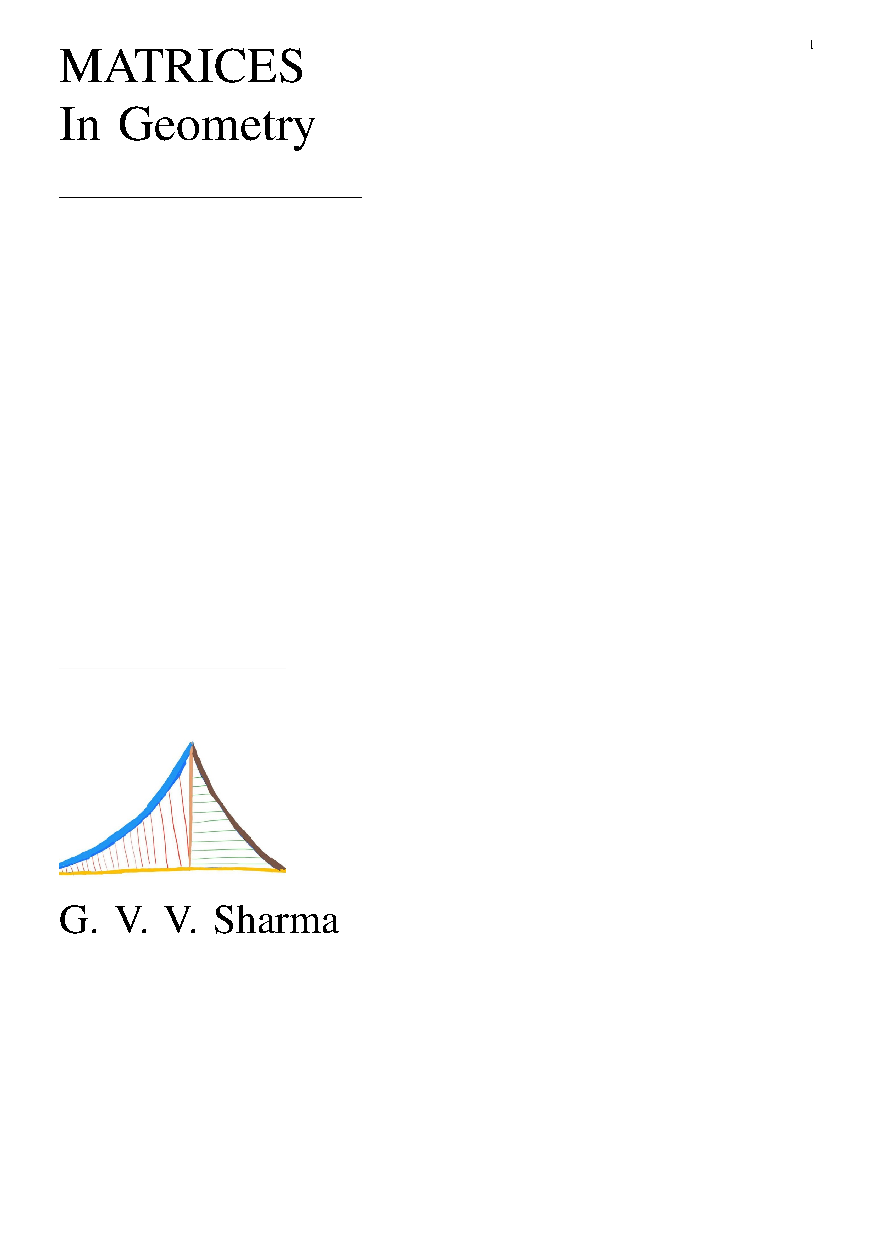
\includegraphics[width=0.75\columnwidth]{chapters/12/6/3/8/figs/main.png}
		\caption{}
		\label{fig:12/6/3/8}
  	\end{figure}
The equation of the conic can be represented as
\begin{align}
\vec{x}^{\top}\myvec{1&0\\0&0}\vec{x}+2\myvec{-2&\frac{-1}{2}}\vec{x}+4=0
\end{align}
So,
\begin{align}
\vec{V}=\myvec{1&0\\0&0},
\vec{u}^{\top}=\myvec{-2&\frac{-1}{2}},
f=4
\end{align}
The direction vector of the line passing through (2,0) and (4,4) is 
\begin{align}
\vec{m}=\myvec{1\\2}
\implies
\vec{n}=\myvec{2\\-1}.
\end{align}
The eigenvector corresponding to the zero eigenvalue is 
\begin{align}
\vec{p}_1=\myvec{0\\1},
\end{align}
In
\eqref{eq:conic_tangent_q_eigen},
\begin{align}
	\kappa=\frac{\myvec{0&1}\myvec{-2\\ \frac{-1}{2}}}{\myvec{0&1}\myvec{2\\-1}}
	=\frac{1}{2}
\end{align}
Substituting  $\kappa$,
from 
\eqref{eq:conic_tangent_q_eigen},
\begin{align}
	\myvec{\sbrak{\myvec{-2\\\frac{-1}{2}}+\frac{1}{2}\myvec{2\\-1}}^{\top} \\ \myvec{1&0\\0&0}}\vec{q} &= \myvec{-4 \\ \frac{1}{2}\myvec{2\\-1}-\myvec{-2\\\frac{-1}{2}}}\\
	\implies
	\myvec{-1&-1 \\ 1&0 \\ 0&0}\vec{q}&=\myvec{-4 \\ 3 \\ 0}
\end{align}
yielding
\begin{align}
\myvec{-1&-1 \\ 1&0}\vec{q} = \myvec{-4\\3}
\end{align}
The augmented matrix is 
\begin{align*}
  \myvec{
                -1&-1&\vrule&-4\\
	        1&0&\vrule&3}
  \xleftrightarrow[]{R_1 \leftarrow R_1+ 2R_2}
     \myvec{
	         1&-1&\vrule&2\\
	         1&0&\vrule&3}
      \\
 \xleftrightarrow[]{R_2 \leftarrow R_2 - R_1}
     \myvec{
	         1&-1&\vrule&2\\
	         0&1&\vrule&1}
 \xleftrightarrow[]{R_1 \leftarrow R_1 + R_2}
     \myvec{
	         1&0&\vrule&3\\
	         0&1&\vrule&1}
      \\ \implies \vec{q}=\myvec{3\\1}
\end{align*}
which is the desired 
point of contact.
See Fig. 
		\ref{fig:12/6/3/8}.



\iffalse
\latexprintindex
\fi

\end{document}


\item   Points $\vec{A}, \vec{B}, \vec{C}$ are defined to be collinear if 
		\begin{align}
			\label{eq:app-app-line-rank}
			\rank{\myvec{1 & 1 & 1 \\ \vec{A}& \vec{B}&\vec{C}}} = 2
		\end{align}
Are the given points in
			\eqref{eq:app-tri-pts}
collinear?
\\
\solution 
From 
			\eqref{eq:app-tri-pts},
\begin{align}
    \label{eq:app-1.1.3,2}
\myvec{
    1 & 1 & 1\\
    \vec{A} & \vec{B} & \vec{C} \\
    } 
    =
    %\label{eq:app-matthrowoperations}
    \myvec{
    1 & 1 & 1
    \\
    1 & -4 & -3
    \\
    -1 & 6 & -5
    }
     \xleftrightarrow[]{R_3 \leftarrow R_3+R_2}
    \myvec{
    1 & 1 & 1
    \\
    1 & -4 & -3
    \\
    0 & 2 & -8 
    }
    \\
     \xleftrightarrow[]{R_2\leftarrow R_1-R_2}
    \myvec{
    1 & 1 & 1
    \\
    0 & 5 & 4
    \\
    0 & 2 & -8 
    }
     \xleftrightarrow[]{R_3\leftarrow R_3-\frac{2}{5}R_2}
    \myvec{
    1 & 1 & 1
    \\
    0 & 5 & 4
    \\
    0 & 0 & \frac{-48}{5}
    }
\end{align}
There are no zero rows. So,
\begin{align}
    \text{rank}\myvec{
    1 & 1 & 1\\
    \vec{A} & \vec{B} & \vec{C} \\
    } &= 3 
\end{align}  
Hence,  the points $\vec{A},\vec{B},\vec{C}$ are not collinear. 
This is visible in 
\figref{fig1:Triangle}.
\begin{figure}[H]
\centering
\includegraphics[width=0.75\columnwidth]{figs/triangle/vector.pdf}
\caption{$\triangle ABC$}
\label{fig1:Triangle}
\end{figure}
% \\		\documentclass[journal]{IEEEtran}
\usepackage{gvv-book}
\usepackage{gvv}
%\usepackage{styles/front}
%\usepackage{Wiley-AuthoringTemplate}
%\usepackage[sectionbib,authoryear]{natbib}% for name-date citation comment the below line
%\usepackage[sectionbib,numbers]{natbib}% for numbered citation comment the above line

%%********************************************************************%%
%%       How many levels of section head would you like numbered?     %%
%% 0= no section numbers, 1= section, 2= section, 3= subsection %%
\setcounter{secnumdepth}{3}
%%********************************************************************%%
%%**********************************************************************%%
%%     How many levels of section head would you like to appear in the  %%
%%				Table of Contents?			%%
%% 0= chapter, 1= section, 2= section, 3= subsection titles.	%%
\setcounter{tocdepth}{2}
%%**********************************************************************%%

%\includeonly{ch01}
\makeindex

\begin{document}
\bibliographystyle{IEEEtran}
\onecolumn


\title{
	\begin{flushleft}
	MATRICES \\ In Geometry
	\\
\rule{0.4\columnwidth}{0.4pt}
\end{flushleft}
}
\author{
\vspace{7cm}
	\begin{flushleft}
\includegraphics[width=0.2\columnwidth]{figs/logo.jpg}
\\
		{	\huge G. V. V. Sharma}
		\\
\vspace{1cm}
https://creativecommons.org/licenses/by-sa/3.0/
\\
and
\\
https://www.gnu.org/licenses/fdl-1.3.en.html
	\end{flushleft}
%\IEEEpubid{\makebox[\columnwidth]{978-1-7281-5966-1/20/\$31.00 ©2020 IEEE \hfill} \hspace{\columnsep}\makebox[\columnwidth]{ }}
}
\maketitle

\newpage


\tableofcontents

\newpage
\twocolumn

%\section{Triangle}
\section{Vectors}
Consider a triangle with vertices
		\begin{align}
			\label{eq:tri-pts}
			\vec{A} = \myvec{1 \\ -1},\,
			\vec{B} = \myvec{-4 \\ 6},\,
			\vec{C} = \myvec{-3 \\ -5}
		\end{align}
\subsection{Sides}
%\renewcommand{\theequation}{\theenumi}
\begin{enumerate}[label=\thesubsection.\arabic*.,ref=\thesubsection.\theenumi]
%\numberwithin{equation}{enumi}
\item The direction vector of $AB$ is defined as
		\begin{align}
			\vec{B}-
			\vec{A}
		\end{align}
Find the direction vectors of $AB, BC$ and $CA$.
\\
\solution 
\begin{enumerate} 
\item  The Direction vector of $AB$ is 
	\begin{align}  \vec{B} - \vec{A} 
		=\myvec{ -4\\ 6 } - \myvec{ 1\\ -1 }
 = \myvec{ -4 - 1\\ 6 - (-1) } = \myvec{ -5\\ 7 }
		\label{eq:app-geo-dir-vec-ab}
 \end{align}
\item The Direction vector of $BC$ is
	\begin{align} \vec{C} - \vec{B}=\myvec{ -3\\ -5} - \myvec{ -4\\ 6 }
 = \myvec{ -3 - (-4)\\ -5 - 6 } = \myvec{1\\ -11 }
		\label{eq:app-geo-dir-vec-bc}
  \end{align}
  \item  The Direction vector of $CA$  is
	  \begin{align}  \vec{A} - \vec{C} =\myvec{ 1\\ -1 }-\myvec{ -3\\ -5}
 = \myvec{ 1 - (-3)\\ -1 - (-5) } = \myvec{ 4\\ 4 }
		\label{eq:app-geo-dir-vec-ca}
  \end{align}
 \end{enumerate}
%	\input{solutions/1/1/1/prob_1.tex}
	\item The length of side $BC$ is 
		\label{prob:side-length}
		\begin{align}
			c = \norm{\vec{B}-\vec{A}} \triangleq \sqrt{\brak{\vec{B}-\vec{A}}^{\top}\brak{\vec{B}-\vec{A}}}
		\end{align}
		where
		\begin{align}
			\vec{A}^{\top}\triangleq\myvec{1 & -1}
		\end{align}
		Similarly, 
		\begin{align}
b = \norm{\vec{C}-\vec{B}},\,
a = \norm{\vec{A}-\vec{C}}
		\end{align}
		Find $a, b, c$.
\begin{enumerate}
	\item 
	From 	
		\eqref{eq:app-geo-dir-vec-ab},
\begin{align}
\vec{A}-\vec{B} &= \myvec{5\\-7}, \\
\implies 	c &= 	\norm{\vec{B}-\vec{A}} = \norm{\vec{A}-\vec{B}} 
	\\
	&= \sqrt{\myvec{5 & -7}\myvec{5\\-7}}
= \sqrt{\brak{5}^2 +\brak{7}^2}\\
	&=\sqrt{74}
		\label{eq:app-geo-norm-ab}
\end{align}
	\item Similarly, from 
		\eqref{eq:app-geo-dir-vec-bc},
\begin{align}
	a &= \norm{\vec{B}-\vec{C}} 
	= \sqrt{\myvec{-1 & 11}\myvec{-1\\11}}
\\
&= \sqrt{\brak{1}^2+\brak{11}^2}
	= \sqrt{122}
		\label{eq:app-geo-norm-bc}
\end{align}
and
		from 		\eqref{eq:app-geo-dir-vec-ca},
	\item 
		\begin{align}
			b &= \norm{\vec{A}-\vec{C}} = \sqrt{\myvec{4 & 4}\myvec{4\\4}}
\\
&= \sqrt{\brak{4}^2+\brak{4}^2}
	=\sqrt{32}
		\label{eq:app-geo-norm-ca}
\end{align}
\end{enumerate}
%  \\            
  %\input{solutions/1/1/2a/main.tex}
\item   Points $\vec{A}, \vec{B}, \vec{C}$ are defined to be collinear if 
		\begin{align}
			\label{eq:app-app-line-rank}
			\rank{\myvec{1 & 1 & 1 \\ \vec{A}& \vec{B}&\vec{C}}} = 2
		\end{align}
Are the given points in
			\eqref{eq:app-tri-pts}
collinear?
\\
\solution 
From 
			\eqref{eq:app-tri-pts},
\begin{align}
    \label{eq:app-1.1.3,2}
\myvec{
    1 & 1 & 1\\
    \vec{A} & \vec{B} & \vec{C} \\
    } 
    =
    %\label{eq:app-matthrowoperations}
    \myvec{
    1 & 1 & 1
    \\
    1 & -4 & -3
    \\
    -1 & 6 & -5
    }
     \xleftrightarrow[]{R_3 \leftarrow R_3+R_2}
    \myvec{
    1 & 1 & 1
    \\
    1 & -4 & -3
    \\
    0 & 2 & -8 
    }
    \\
     \xleftrightarrow[]{R_2\leftarrow R_1-R_2}
    \myvec{
    1 & 1 & 1
    \\
    0 & 5 & 4
    \\
    0 & 2 & -8 
    }
     \xleftrightarrow[]{R_3\leftarrow R_3-\frac{2}{5}R_2}
    \myvec{
    1 & 1 & 1
    \\
    0 & 5 & 4
    \\
    0 & 0 & \frac{-48}{5}
    }
\end{align}
There are no zero rows. So,
\begin{align}
    \text{rank}\myvec{
    1 & 1 & 1\\
    \vec{A} & \vec{B} & \vec{C} \\
    } &= 3 
\end{align}  
Hence,  the points $\vec{A},\vec{B},\vec{C}$ are not collinear. 
This is visible in 
\figref{fig1:Triangle}.
\begin{figure}[H]
\centering
\includegraphics[width=0.75\columnwidth]{figs/triangle/vector.pdf}
\caption{$\triangle ABC$}
\label{fig1:Triangle}
\end{figure}
% \\		\input{solutions/1/1/3/main.tex}
\item The parameteric form of the equation  of $AB$ is 
		\begin{align}
			\label{eq:app-geo-param}
			\vec{x}=\vec{A}+k\vec{m} \quad k \ne 0,
		\end{align}
		where
		\begin{align}
\vec{m}=\vec{B}-\vec{A}
		\end{align}
is the direction vector of $AB$.
Find the parameteric equations of $AB, BC$ and $CA$.
\\
\solution
From 
			\eqref{eq:app-geo-param} and
		\eqref{eq:app-geo-dir-vec-ab},
the parametric equation for $AB$ is given by
\begin{align}
AB: \vec{x} = &\myvec{1\\-1} + k \myvec{-5\\7}
\end{align}
Similarly, from 
		\eqref{eq:app-geo-dir-vec-bc} and
		\eqref{eq:app-geo-dir-vec-ca},
\begin{align}
BC: \vec{x} = &\myvec{-4\\6} + k \myvec{1\\-11}\\
CA: \vec{x} = &\myvec{-3\\-5} + k \myvec{4\\4}
\end{align}

%		\input{solutions/1/1/4/main.tex}
\item The normal form of the equation of $AB$  is 
		\begin{align}
			\label{eq:app-geo-normal}
			\vec{n}^{\top}\brak{	\vec{x}-\vec{A}} = 0
		\end{align}
		where 
		\begin{align}
			\vec{n}^{\top}\vec{m}&=\vec{n}^{\top}\brak{\vec{B}-\vec{A}} = 0
			\\
			\text{or, } \vec{n}&=\myvec{0 & 1 \\ -1 & 0} \vec{m}
			\label{eq:app-geo-norm-vec}
		\end{align}
Find the normal form of the equations of $AB, BC$ and $CA$.
\\
\solution
\begin{enumerate}
	\item
From
		\eqref{eq:app-geo-dir-vec-bc}, 
the direction vector of side $\vec{BC}$ is
\begin{align}
\vec{m}
	&=\myvec{1\\-11}
	\\
\implies \vec{n} &= \myvec{0 & 1\\
  -1 & 0}\myvec{1\\-11}
 = \myvec{-11\\-1}
		\label{eq:app-geo-norm-vec-bc}
\end{align}
from 
			\eqref{eq:app-geo-norm-vec}.
Hence, from 
			\eqref{eq:app-geo-normal},
the normal equation of side $BC$ is 
\begin{align}
	\vec{n}^{\top}\brak{	\vec{x}-\vec{B}} &= 0
			\\
\implies    \myvec{-11 & -1}\vec{x}&=\myvec{-11 & -1}\myvec{-4\\6}\\
    \implies
BC: \quad    \myvec{11 & 1}\vec{x}&=-38
\end{align}
\item Similarly, for $AB$,
from 
		\eqref{eq:app-geo-dir-vec-ab}, 
\begin{align}
	\vec{m} &= \myvec{-5\\7}
	\\
\implies        \vec{n} 
                &= \myvec{0&1\\-1&0}\myvec{-5\\7}
                = \myvec{7\\5}
		\label{eq:app-geo-norm-vec-ab}
\end{align}
and 
\begin{align}
	\vec{n}^{\top}\brak{	\vec{x}-\vec{A}} &= 0
	\\
	\implies
                AB: \quad  \vec{n}^{\top}\vec{x} &= \myvec{7&5}\myvec{1\\-1}\\    
       \implies\myvec{7&5}\vec{x} &= 2
\end{align}
\item For 
$CA$, 
from 
		\eqref{eq:app-geo-dir-vec-ca}, 
\begin{align}
\vec{m} &= \myvec{1 \\ 1}
\\
		\label{eq:app-geo-norm-vec-ca}
\implies \vec{n} 
&= \myvec{0&1 \\ -1&0}\myvec{1 \\ 1}
= \myvec{1 \\ -1}\\
\\
\implies	\vec{n}^{\top}\brak{	\vec{x}-\vec{C}} &= 0
\\
\implies \myvec{1&-1}{\vec{x}} &= \myvec{1&-1}\myvec{-3 \\ -5} 
= 2 
\end{align}
\end{enumerate}

%\input{solutions/1/1/5/assign1.tex}
\item The area of $\triangle ABC$ is defined as
		\begin{align}
			\label{eq:app-tri-area-cross}
			\frac{1}{2}\norm{{\brak{\vec{A}-\vec{B}}\times \brak{\vec{A}-\vec{C}}}}
		\end{align}
		where
		\begin{align}
			\vec{A}\times\vec{B} \triangleq \mydet{1 & -4 \\-1 & 6}
		\end{align}
		Find the area of $\triangle ABC$.\\
\solution
From
		\eqref{eq:app-geo-dir-vec-ab}
		and
		\eqref{eq:app-geo-dir-vec-ca},
\begin{align}
	\vec{A}-\vec{B}=\myvec{5\\-7},
	\vec{A}-\vec{C}&=\myvec{4\\4}\\
\implies (\vec{A}-\vec{B})\times(\vec{A}-\vec{C}) &=\mydet{5 & 4\\-7 & 4}\\
&=5\times 4-4\times (-7)\\&=48\\
\implies\frac{1}{2}\norm{(\vec{A}-\vec{B})\times(\vec{A}-\vec{C})}&=\frac{48}{2}=24
\end{align}
which is the desired area.

%  		\input{solutions/1/1/6/main.tex}
	\item Find the angles $A, B, C$ if 
%    \label{prop:angle2d}
  \begin{align}
    \label{eq:app-angle2d}
			\cos A \triangleq 
\frac{\brak{\vec{B}-\vec{A}}^{\top}{\vec{C}-\vec{A}}}{\norm{\vec{B}-\vec{A}}\norm{\vec{C}-\vec{A}}}
  \end{align}\\
  \solution
\begin{enumerate}
	\item From 
		\eqref{eq:app-geo-dir-vec-ab},
		\eqref{eq:app-geo-dir-vec-ca},
		\eqref{eq:app-geo-norm-ab}
		and
		\eqref{eq:app-geo-norm-ca}
\begin{align}
	(\vec{B}-\vec{A})^{\top}(\vec{C}-\vec{A})&=\myvec{-5&7}\myvec{-4\\-4}\\
	&=-8
	\\
	\implies
	\cos{A}&= \frac{-8}{\sqrt{74} \sqrt{32}}
	= \frac{-1}{\sqrt{37}}\\
	\implies A&=\cos^{-1}{\frac{-1}{\sqrt{37}}}
\end{align}
	\item From 
		\eqref{eq:app-geo-dir-vec-ab},
		\eqref{eq:app-geo-dir-vec-bc},
		\eqref{eq:app-geo-norm-ab}
		and
		\eqref{eq:app-geo-norm-bc}
\begin{align}
	(\vec{C}-\vec{B})^{\top}(\vec{A}-\vec{B})&=\myvec{1&-11}\myvec{5\\-7}\\
	&= 82
	\\
	\implies
	\cos{B}&= \frac{82}{\sqrt{74} \sqrt{122}}
	= \frac{41}{\sqrt{2257}}\\
	\implies B&=\cos^{-1}{\frac{41}{\sqrt{2257}}}
\end{align}
	\item From 
		\eqref{eq:app-geo-dir-vec-bc},
		\eqref{eq:app-geo-dir-vec-ca},
		\eqref{eq:app-geo-norm-bc}
		and
		\eqref{eq:app-geo-norm-ca}
\begin{align}
	(\vec{A}-\vec{C})^{\top}(\vec{B}-\vec{C})&=\myvec{4&4}\myvec{-1\\11}\\
	&=40
	\\
\implies	\cos{C}&= \frac{40}{\sqrt{32} \sqrt{122}}
	= \frac{5}{\sqrt{61}}\\
	\implies C&=\cos^{-1}{\frac{5}{\sqrt{61}}}
\end{align}

\end{enumerate}
%  	\input{solutions/1/1/7/main.tex}
All codes for this section are available at
\begin{lstlisting}
	codes/triangle/sides.py
\end{lstlisting}
\end{enumerate}

\subsection{Median}
\input{chapters/triangle/median}
\subsection{Altitude}
\input{chapters/triangle/altitude}
\subsection{Perpendicular Bisector}
\input{chapters/triangle/perp-bisect}
\subsection{Angle Bisector}
\input{chapters/triangle/angle-bisect}
\subsection{Eigenvalues and Eigenvectors}
\input{chapters/triangle/eigen}
\section{Matrices}
The mid point of $PB$ is
\begin{align}
\vec{M} =\frac{1}{2}(\vec{P}+\vec{B})
	= \myvec{4 \\ -2}  
\end{align}
which is equal to the direction vector of $OM$.
\begin{align}
\because \vec{M} \equiv
	 \myvec{1 \\ -\frac{1}{2}},
	m = -\frac{1}{2}
\end{align}
which is the desired slope.
See 
		\figref{fig:11/10/1/5}.
	\begin{figure}[!ht]
		\centering
 \includegraphics[width=\columnwidth]{chapters/11/10/1/5/figs/line.png}
		\caption{}
		\label{fig:11/10/1/5}
  	\end{figure}


%\section{Quadrilateral}
%\input{./chapters/exercises/quad_geo_exer}

\appendices
\section{Tangents to a Circle}
\numberwithin{equation}{section}
	\begin{figure}[H]
		\centering
 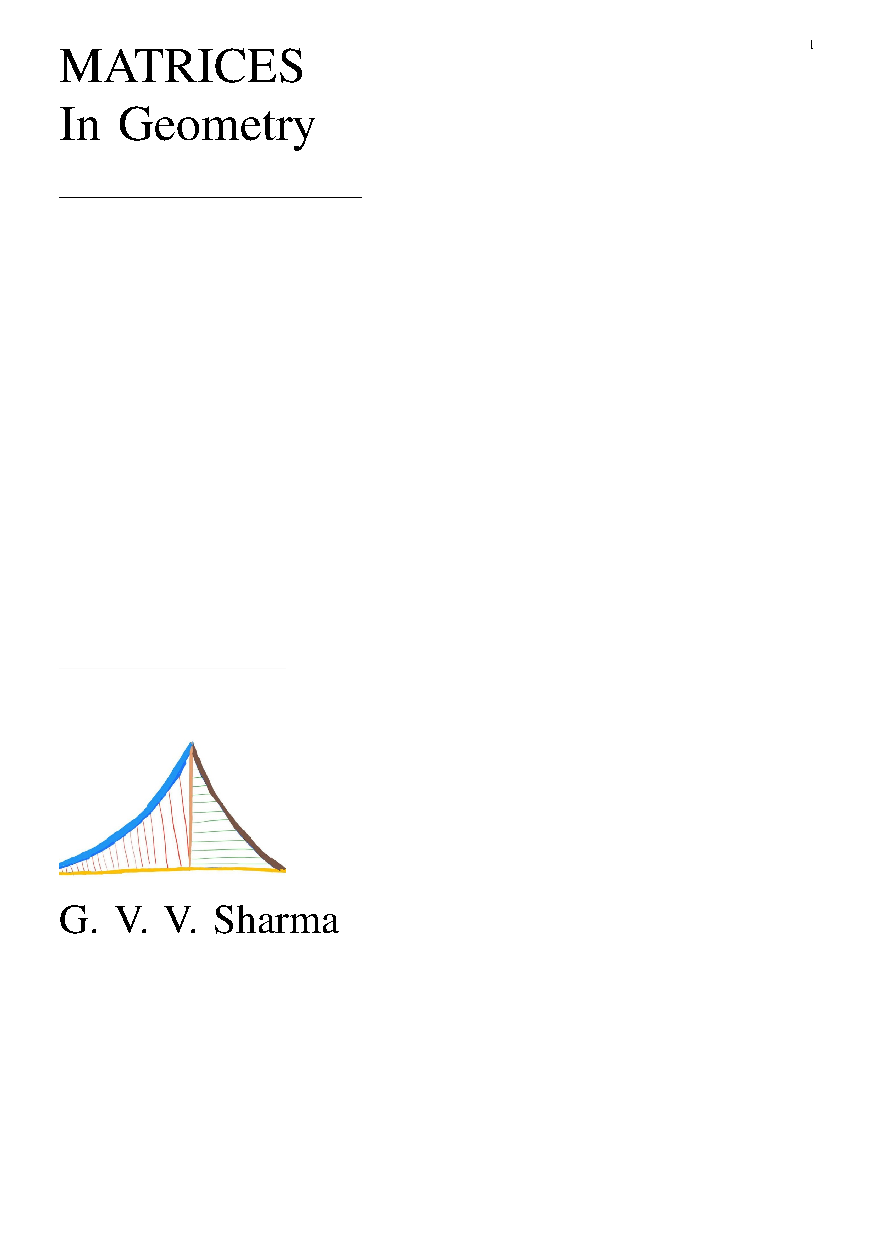
\includegraphics[width=0.75\columnwidth]{chapters/12/6/3/8/figs/main.png}
		\caption{}
		\label{fig:12/6/3/8}
  	\end{figure}
The equation of the conic can be represented as
\begin{align}
\vec{x}^{\top}\myvec{1&0\\0&0}\vec{x}+2\myvec{-2&\frac{-1}{2}}\vec{x}+4=0
\end{align}
So,
\begin{align}
\vec{V}=\myvec{1&0\\0&0},
\vec{u}^{\top}=\myvec{-2&\frac{-1}{2}},
f=4
\end{align}
The direction vector of the line passing through (2,0) and (4,4) is 
\begin{align}
\vec{m}=\myvec{1\\2}
\implies
\vec{n}=\myvec{2\\-1}.
\end{align}
The eigenvector corresponding to the zero eigenvalue is 
\begin{align}
\vec{p}_1=\myvec{0\\1},
\end{align}
In
\eqref{eq:conic_tangent_q_eigen},
\begin{align}
	\kappa=\frac{\myvec{0&1}\myvec{-2\\ \frac{-1}{2}}}{\myvec{0&1}\myvec{2\\-1}}
	=\frac{1}{2}
\end{align}
Substituting  $\kappa$,
from 
\eqref{eq:conic_tangent_q_eigen},
\begin{align}
	\myvec{\sbrak{\myvec{-2\\\frac{-1}{2}}+\frac{1}{2}\myvec{2\\-1}}^{\top} \\ \myvec{1&0\\0&0}}\vec{q} &= \myvec{-4 \\ \frac{1}{2}\myvec{2\\-1}-\myvec{-2\\\frac{-1}{2}}}\\
	\implies
	\myvec{-1&-1 \\ 1&0 \\ 0&0}\vec{q}&=\myvec{-4 \\ 3 \\ 0}
\end{align}
yielding
\begin{align}
\myvec{-1&-1 \\ 1&0}\vec{q} = \myvec{-4\\3}
\end{align}
The augmented matrix is 
\begin{align*}
  \myvec{
                -1&-1&\vrule&-4\\
	        1&0&\vrule&3}
  \xleftrightarrow[]{R_1 \leftarrow R_1+ 2R_2}
     \myvec{
	         1&-1&\vrule&2\\
	         1&0&\vrule&3}
      \\
 \xleftrightarrow[]{R_2 \leftarrow R_2 - R_1}
     \myvec{
	         1&-1&\vrule&2\\
	         0&1&\vrule&1}
 \xleftrightarrow[]{R_1 \leftarrow R_1 + R_2}
     \myvec{
	         1&0&\vrule&3\\
	         0&1&\vrule&1}
      \\ \implies \vec{q}=\myvec{3\\1}
\end{align*}
which is the desired 
point of contact.
See Fig. 
		\ref{fig:12/6/3/8}.



\iffalse
\latexprintindex
\fi

\end{document}


\item The parameteric form of the equation  of $AB$ is 
		\begin{align}
			\label{eq:app-geo-param}
			\vec{x}=\vec{A}+k\vec{m} \quad k \ne 0,
		\end{align}
		where
		\begin{align}
\vec{m}=\vec{B}-\vec{A}
		\end{align}
is the direction vector of $AB$.
Find the parameteric equations of $AB, BC$ and $CA$.
\\
\solution
From 
			\eqref{eq:app-geo-param} and
		\eqref{eq:app-geo-dir-vec-ab},
the parametric equation for $AB$ is given by
\begin{align}
AB: \vec{x} = &\myvec{1\\-1} + k \myvec{-5\\7}
\end{align}
Similarly, from 
		\eqref{eq:app-geo-dir-vec-bc} and
		\eqref{eq:app-geo-dir-vec-ca},
\begin{align}
BC: \vec{x} = &\myvec{-4\\6} + k \myvec{1\\-11}\\
CA: \vec{x} = &\myvec{-3\\-5} + k \myvec{4\\4}
\end{align}

%		\documentclass[journal]{IEEEtran}
\usepackage{gvv-book}
\usepackage{gvv}
%\usepackage{styles/front}
%\usepackage{Wiley-AuthoringTemplate}
%\usepackage[sectionbib,authoryear]{natbib}% for name-date citation comment the below line
%\usepackage[sectionbib,numbers]{natbib}% for numbered citation comment the above line

%%********************************************************************%%
%%       How many levels of section head would you like numbered?     %%
%% 0= no section numbers, 1= section, 2= section, 3= subsection %%
\setcounter{secnumdepth}{3}
%%********************************************************************%%
%%**********************************************************************%%
%%     How many levels of section head would you like to appear in the  %%
%%				Table of Contents?			%%
%% 0= chapter, 1= section, 2= section, 3= subsection titles.	%%
\setcounter{tocdepth}{2}
%%**********************************************************************%%

%\includeonly{ch01}
\makeindex

\begin{document}
\bibliographystyle{IEEEtran}
\onecolumn


\title{
	\begin{flushleft}
	MATRICES \\ In Geometry
	\\
\rule{0.4\columnwidth}{0.4pt}
\end{flushleft}
}
\author{
\vspace{7cm}
	\begin{flushleft}
\includegraphics[width=0.2\columnwidth]{figs/logo.jpg}
\\
		{	\huge G. V. V. Sharma}
		\\
\vspace{1cm}
https://creativecommons.org/licenses/by-sa/3.0/
\\
and
\\
https://www.gnu.org/licenses/fdl-1.3.en.html
	\end{flushleft}
%\IEEEpubid{\makebox[\columnwidth]{978-1-7281-5966-1/20/\$31.00 ©2020 IEEE \hfill} \hspace{\columnsep}\makebox[\columnwidth]{ }}
}
\maketitle

\newpage


\tableofcontents

\newpage
\twocolumn

%\section{Triangle}
\section{Vectors}
Consider a triangle with vertices
		\begin{align}
			\label{eq:tri-pts}
			\vec{A} = \myvec{1 \\ -1},\,
			\vec{B} = \myvec{-4 \\ 6},\,
			\vec{C} = \myvec{-3 \\ -5}
		\end{align}
\subsection{Sides}
%\renewcommand{\theequation}{\theenumi}
\begin{enumerate}[label=\thesubsection.\arabic*.,ref=\thesubsection.\theenumi]
%\numberwithin{equation}{enumi}
\item The direction vector of $AB$ is defined as
		\begin{align}
			\vec{B}-
			\vec{A}
		\end{align}
Find the direction vectors of $AB, BC$ and $CA$.
\\
\solution 
\begin{enumerate} 
\item  The Direction vector of $AB$ is 
	\begin{align}  \vec{B} - \vec{A} 
		=\myvec{ -4\\ 6 } - \myvec{ 1\\ -1 }
 = \myvec{ -4 - 1\\ 6 - (-1) } = \myvec{ -5\\ 7 }
		\label{eq:app-geo-dir-vec-ab}
 \end{align}
\item The Direction vector of $BC$ is
	\begin{align} \vec{C} - \vec{B}=\myvec{ -3\\ -5} - \myvec{ -4\\ 6 }
 = \myvec{ -3 - (-4)\\ -5 - 6 } = \myvec{1\\ -11 }
		\label{eq:app-geo-dir-vec-bc}
  \end{align}
  \item  The Direction vector of $CA$  is
	  \begin{align}  \vec{A} - \vec{C} =\myvec{ 1\\ -1 }-\myvec{ -3\\ -5}
 = \myvec{ 1 - (-3)\\ -1 - (-5) } = \myvec{ 4\\ 4 }
		\label{eq:app-geo-dir-vec-ca}
  \end{align}
 \end{enumerate}
%	\input{solutions/1/1/1/prob_1.tex}
	\item The length of side $BC$ is 
		\label{prob:side-length}
		\begin{align}
			c = \norm{\vec{B}-\vec{A}} \triangleq \sqrt{\brak{\vec{B}-\vec{A}}^{\top}\brak{\vec{B}-\vec{A}}}
		\end{align}
		where
		\begin{align}
			\vec{A}^{\top}\triangleq\myvec{1 & -1}
		\end{align}
		Similarly, 
		\begin{align}
b = \norm{\vec{C}-\vec{B}},\,
a = \norm{\vec{A}-\vec{C}}
		\end{align}
		Find $a, b, c$.
\begin{enumerate}
	\item 
	From 	
		\eqref{eq:app-geo-dir-vec-ab},
\begin{align}
\vec{A}-\vec{B} &= \myvec{5\\-7}, \\
\implies 	c &= 	\norm{\vec{B}-\vec{A}} = \norm{\vec{A}-\vec{B}} 
	\\
	&= \sqrt{\myvec{5 & -7}\myvec{5\\-7}}
= \sqrt{\brak{5}^2 +\brak{7}^2}\\
	&=\sqrt{74}
		\label{eq:app-geo-norm-ab}
\end{align}
	\item Similarly, from 
		\eqref{eq:app-geo-dir-vec-bc},
\begin{align}
	a &= \norm{\vec{B}-\vec{C}} 
	= \sqrt{\myvec{-1 & 11}\myvec{-1\\11}}
\\
&= \sqrt{\brak{1}^2+\brak{11}^2}
	= \sqrt{122}
		\label{eq:app-geo-norm-bc}
\end{align}
and
		from 		\eqref{eq:app-geo-dir-vec-ca},
	\item 
		\begin{align}
			b &= \norm{\vec{A}-\vec{C}} = \sqrt{\myvec{4 & 4}\myvec{4\\4}}
\\
&= \sqrt{\brak{4}^2+\brak{4}^2}
	=\sqrt{32}
		\label{eq:app-geo-norm-ca}
\end{align}
\end{enumerate}
%  \\            
  %\input{solutions/1/1/2a/main.tex}
\item   Points $\vec{A}, \vec{B}, \vec{C}$ are defined to be collinear if 
		\begin{align}
			\label{eq:app-app-line-rank}
			\rank{\myvec{1 & 1 & 1 \\ \vec{A}& \vec{B}&\vec{C}}} = 2
		\end{align}
Are the given points in
			\eqref{eq:app-tri-pts}
collinear?
\\
\solution 
From 
			\eqref{eq:app-tri-pts},
\begin{align}
    \label{eq:app-1.1.3,2}
\myvec{
    1 & 1 & 1\\
    \vec{A} & \vec{B} & \vec{C} \\
    } 
    =
    %\label{eq:app-matthrowoperations}
    \myvec{
    1 & 1 & 1
    \\
    1 & -4 & -3
    \\
    -1 & 6 & -5
    }
     \xleftrightarrow[]{R_3 \leftarrow R_3+R_2}
    \myvec{
    1 & 1 & 1
    \\
    1 & -4 & -3
    \\
    0 & 2 & -8 
    }
    \\
     \xleftrightarrow[]{R_2\leftarrow R_1-R_2}
    \myvec{
    1 & 1 & 1
    \\
    0 & 5 & 4
    \\
    0 & 2 & -8 
    }
     \xleftrightarrow[]{R_3\leftarrow R_3-\frac{2}{5}R_2}
    \myvec{
    1 & 1 & 1
    \\
    0 & 5 & 4
    \\
    0 & 0 & \frac{-48}{5}
    }
\end{align}
There are no zero rows. So,
\begin{align}
    \text{rank}\myvec{
    1 & 1 & 1\\
    \vec{A} & \vec{B} & \vec{C} \\
    } &= 3 
\end{align}  
Hence,  the points $\vec{A},\vec{B},\vec{C}$ are not collinear. 
This is visible in 
\figref{fig1:Triangle}.
\begin{figure}[H]
\centering
\includegraphics[width=0.75\columnwidth]{figs/triangle/vector.pdf}
\caption{$\triangle ABC$}
\label{fig1:Triangle}
\end{figure}
% \\		\input{solutions/1/1/3/main.tex}
\item The parameteric form of the equation  of $AB$ is 
		\begin{align}
			\label{eq:app-geo-param}
			\vec{x}=\vec{A}+k\vec{m} \quad k \ne 0,
		\end{align}
		where
		\begin{align}
\vec{m}=\vec{B}-\vec{A}
		\end{align}
is the direction vector of $AB$.
Find the parameteric equations of $AB, BC$ and $CA$.
\\
\solution
From 
			\eqref{eq:app-geo-param} and
		\eqref{eq:app-geo-dir-vec-ab},
the parametric equation for $AB$ is given by
\begin{align}
AB: \vec{x} = &\myvec{1\\-1} + k \myvec{-5\\7}
\end{align}
Similarly, from 
		\eqref{eq:app-geo-dir-vec-bc} and
		\eqref{eq:app-geo-dir-vec-ca},
\begin{align}
BC: \vec{x} = &\myvec{-4\\6} + k \myvec{1\\-11}\\
CA: \vec{x} = &\myvec{-3\\-5} + k \myvec{4\\4}
\end{align}

%		\input{solutions/1/1/4/main.tex}
\item The normal form of the equation of $AB$  is 
		\begin{align}
			\label{eq:app-geo-normal}
			\vec{n}^{\top}\brak{	\vec{x}-\vec{A}} = 0
		\end{align}
		where 
		\begin{align}
			\vec{n}^{\top}\vec{m}&=\vec{n}^{\top}\brak{\vec{B}-\vec{A}} = 0
			\\
			\text{or, } \vec{n}&=\myvec{0 & 1 \\ -1 & 0} \vec{m}
			\label{eq:app-geo-norm-vec}
		\end{align}
Find the normal form of the equations of $AB, BC$ and $CA$.
\\
\solution
\begin{enumerate}
	\item
From
		\eqref{eq:app-geo-dir-vec-bc}, 
the direction vector of side $\vec{BC}$ is
\begin{align}
\vec{m}
	&=\myvec{1\\-11}
	\\
\implies \vec{n} &= \myvec{0 & 1\\
  -1 & 0}\myvec{1\\-11}
 = \myvec{-11\\-1}
		\label{eq:app-geo-norm-vec-bc}
\end{align}
from 
			\eqref{eq:app-geo-norm-vec}.
Hence, from 
			\eqref{eq:app-geo-normal},
the normal equation of side $BC$ is 
\begin{align}
	\vec{n}^{\top}\brak{	\vec{x}-\vec{B}} &= 0
			\\
\implies    \myvec{-11 & -1}\vec{x}&=\myvec{-11 & -1}\myvec{-4\\6}\\
    \implies
BC: \quad    \myvec{11 & 1}\vec{x}&=-38
\end{align}
\item Similarly, for $AB$,
from 
		\eqref{eq:app-geo-dir-vec-ab}, 
\begin{align}
	\vec{m} &= \myvec{-5\\7}
	\\
\implies        \vec{n} 
                &= \myvec{0&1\\-1&0}\myvec{-5\\7}
                = \myvec{7\\5}
		\label{eq:app-geo-norm-vec-ab}
\end{align}
and 
\begin{align}
	\vec{n}^{\top}\brak{	\vec{x}-\vec{A}} &= 0
	\\
	\implies
                AB: \quad  \vec{n}^{\top}\vec{x} &= \myvec{7&5}\myvec{1\\-1}\\    
       \implies\myvec{7&5}\vec{x} &= 2
\end{align}
\item For 
$CA$, 
from 
		\eqref{eq:app-geo-dir-vec-ca}, 
\begin{align}
\vec{m} &= \myvec{1 \\ 1}
\\
		\label{eq:app-geo-norm-vec-ca}
\implies \vec{n} 
&= \myvec{0&1 \\ -1&0}\myvec{1 \\ 1}
= \myvec{1 \\ -1}\\
\\
\implies	\vec{n}^{\top}\brak{	\vec{x}-\vec{C}} &= 0
\\
\implies \myvec{1&-1}{\vec{x}} &= \myvec{1&-1}\myvec{-3 \\ -5} 
= 2 
\end{align}
\end{enumerate}

%\input{solutions/1/1/5/assign1.tex}
\item The area of $\triangle ABC$ is defined as
		\begin{align}
			\label{eq:app-tri-area-cross}
			\frac{1}{2}\norm{{\brak{\vec{A}-\vec{B}}\times \brak{\vec{A}-\vec{C}}}}
		\end{align}
		where
		\begin{align}
			\vec{A}\times\vec{B} \triangleq \mydet{1 & -4 \\-1 & 6}
		\end{align}
		Find the area of $\triangle ABC$.\\
\solution
From
		\eqref{eq:app-geo-dir-vec-ab}
		and
		\eqref{eq:app-geo-dir-vec-ca},
\begin{align}
	\vec{A}-\vec{B}=\myvec{5\\-7},
	\vec{A}-\vec{C}&=\myvec{4\\4}\\
\implies (\vec{A}-\vec{B})\times(\vec{A}-\vec{C}) &=\mydet{5 & 4\\-7 & 4}\\
&=5\times 4-4\times (-7)\\&=48\\
\implies\frac{1}{2}\norm{(\vec{A}-\vec{B})\times(\vec{A}-\vec{C})}&=\frac{48}{2}=24
\end{align}
which is the desired area.

%  		\input{solutions/1/1/6/main.tex}
	\item Find the angles $A, B, C$ if 
%    \label{prop:angle2d}
  \begin{align}
    \label{eq:app-angle2d}
			\cos A \triangleq 
\frac{\brak{\vec{B}-\vec{A}}^{\top}{\vec{C}-\vec{A}}}{\norm{\vec{B}-\vec{A}}\norm{\vec{C}-\vec{A}}}
  \end{align}\\
  \solution
\begin{enumerate}
	\item From 
		\eqref{eq:app-geo-dir-vec-ab},
		\eqref{eq:app-geo-dir-vec-ca},
		\eqref{eq:app-geo-norm-ab}
		and
		\eqref{eq:app-geo-norm-ca}
\begin{align}
	(\vec{B}-\vec{A})^{\top}(\vec{C}-\vec{A})&=\myvec{-5&7}\myvec{-4\\-4}\\
	&=-8
	\\
	\implies
	\cos{A}&= \frac{-8}{\sqrt{74} \sqrt{32}}
	= \frac{-1}{\sqrt{37}}\\
	\implies A&=\cos^{-1}{\frac{-1}{\sqrt{37}}}
\end{align}
	\item From 
		\eqref{eq:app-geo-dir-vec-ab},
		\eqref{eq:app-geo-dir-vec-bc},
		\eqref{eq:app-geo-norm-ab}
		and
		\eqref{eq:app-geo-norm-bc}
\begin{align}
	(\vec{C}-\vec{B})^{\top}(\vec{A}-\vec{B})&=\myvec{1&-11}\myvec{5\\-7}\\
	&= 82
	\\
	\implies
	\cos{B}&= \frac{82}{\sqrt{74} \sqrt{122}}
	= \frac{41}{\sqrt{2257}}\\
	\implies B&=\cos^{-1}{\frac{41}{\sqrt{2257}}}
\end{align}
	\item From 
		\eqref{eq:app-geo-dir-vec-bc},
		\eqref{eq:app-geo-dir-vec-ca},
		\eqref{eq:app-geo-norm-bc}
		and
		\eqref{eq:app-geo-norm-ca}
\begin{align}
	(\vec{A}-\vec{C})^{\top}(\vec{B}-\vec{C})&=\myvec{4&4}\myvec{-1\\11}\\
	&=40
	\\
\implies	\cos{C}&= \frac{40}{\sqrt{32} \sqrt{122}}
	= \frac{5}{\sqrt{61}}\\
	\implies C&=\cos^{-1}{\frac{5}{\sqrt{61}}}
\end{align}

\end{enumerate}
%  	\input{solutions/1/1/7/main.tex}
All codes for this section are available at
\begin{lstlisting}
	codes/triangle/sides.py
\end{lstlisting}
\end{enumerate}

\subsection{Median}
\input{chapters/triangle/median}
\subsection{Altitude}
\input{chapters/triangle/altitude}
\subsection{Perpendicular Bisector}
\input{chapters/triangle/perp-bisect}
\subsection{Angle Bisector}
\input{chapters/triangle/angle-bisect}
\subsection{Eigenvalues and Eigenvectors}
\input{chapters/triangle/eigen}
\section{Matrices}
The mid point of $PB$ is
\begin{align}
\vec{M} =\frac{1}{2}(\vec{P}+\vec{B})
	= \myvec{4 \\ -2}  
\end{align}
which is equal to the direction vector of $OM$.
\begin{align}
\because \vec{M} \equiv
	 \myvec{1 \\ -\frac{1}{2}},
	m = -\frac{1}{2}
\end{align}
which is the desired slope.
See 
		\figref{fig:11/10/1/5}.
	\begin{figure}[!ht]
		\centering
 \includegraphics[width=\columnwidth]{chapters/11/10/1/5/figs/line.png}
		\caption{}
		\label{fig:11/10/1/5}
  	\end{figure}


%\section{Quadrilateral}
%\input{./chapters/exercises/quad_geo_exer}

\appendices
\section{Tangents to a Circle}
\numberwithin{equation}{section}
	\begin{figure}[H]
		\centering
 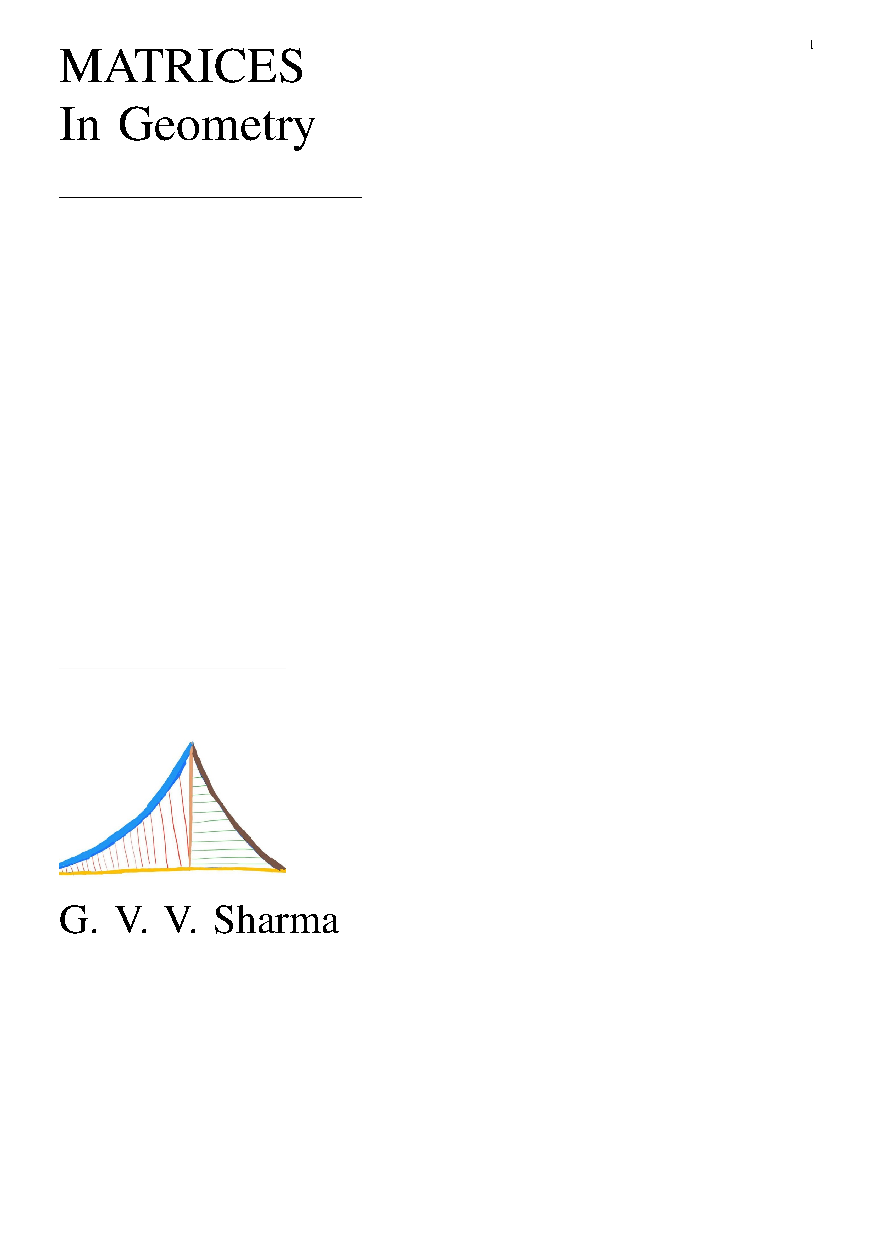
\includegraphics[width=0.75\columnwidth]{chapters/12/6/3/8/figs/main.png}
		\caption{}
		\label{fig:12/6/3/8}
  	\end{figure}
The equation of the conic can be represented as
\begin{align}
\vec{x}^{\top}\myvec{1&0\\0&0}\vec{x}+2\myvec{-2&\frac{-1}{2}}\vec{x}+4=0
\end{align}
So,
\begin{align}
\vec{V}=\myvec{1&0\\0&0},
\vec{u}^{\top}=\myvec{-2&\frac{-1}{2}},
f=4
\end{align}
The direction vector of the line passing through (2,0) and (4,4) is 
\begin{align}
\vec{m}=\myvec{1\\2}
\implies
\vec{n}=\myvec{2\\-1}.
\end{align}
The eigenvector corresponding to the zero eigenvalue is 
\begin{align}
\vec{p}_1=\myvec{0\\1},
\end{align}
In
\eqref{eq:conic_tangent_q_eigen},
\begin{align}
	\kappa=\frac{\myvec{0&1}\myvec{-2\\ \frac{-1}{2}}}{\myvec{0&1}\myvec{2\\-1}}
	=\frac{1}{2}
\end{align}
Substituting  $\kappa$,
from 
\eqref{eq:conic_tangent_q_eigen},
\begin{align}
	\myvec{\sbrak{\myvec{-2\\\frac{-1}{2}}+\frac{1}{2}\myvec{2\\-1}}^{\top} \\ \myvec{1&0\\0&0}}\vec{q} &= \myvec{-4 \\ \frac{1}{2}\myvec{2\\-1}-\myvec{-2\\\frac{-1}{2}}}\\
	\implies
	\myvec{-1&-1 \\ 1&0 \\ 0&0}\vec{q}&=\myvec{-4 \\ 3 \\ 0}
\end{align}
yielding
\begin{align}
\myvec{-1&-1 \\ 1&0}\vec{q} = \myvec{-4\\3}
\end{align}
The augmented matrix is 
\begin{align*}
  \myvec{
                -1&-1&\vrule&-4\\
	        1&0&\vrule&3}
  \xleftrightarrow[]{R_1 \leftarrow R_1+ 2R_2}
     \myvec{
	         1&-1&\vrule&2\\
	         1&0&\vrule&3}
      \\
 \xleftrightarrow[]{R_2 \leftarrow R_2 - R_1}
     \myvec{
	         1&-1&\vrule&2\\
	         0&1&\vrule&1}
 \xleftrightarrow[]{R_1 \leftarrow R_1 + R_2}
     \myvec{
	         1&0&\vrule&3\\
	         0&1&\vrule&1}
      \\ \implies \vec{q}=\myvec{3\\1}
\end{align*}
which is the desired 
point of contact.
See Fig. 
		\ref{fig:12/6/3/8}.



\iffalse
\latexprintindex
\fi

\end{document}


\item The normal form of the equation of $AB$  is 
		\begin{align}
			\label{eq:app-geo-normal}
			\vec{n}^{\top}\brak{	\vec{x}-\vec{A}} = 0
		\end{align}
		where 
		\begin{align}
			\vec{n}^{\top}\vec{m}&=\vec{n}^{\top}\brak{\vec{B}-\vec{A}} = 0
			\\
			\text{or, } \vec{n}&=\myvec{0 & 1 \\ -1 & 0} \vec{m}
			\label{eq:app-geo-norm-vec}
		\end{align}
Find the normal form of the equations of $AB, BC$ and $CA$.
\\
\solution
\begin{enumerate}
	\item
From
		\eqref{eq:app-geo-dir-vec-bc}, 
the direction vector of side $\vec{BC}$ is
\begin{align}
\vec{m}
	&=\myvec{1\\-11}
	\\
\implies \vec{n} &= \myvec{0 & 1\\
  -1 & 0}\myvec{1\\-11}
 = \myvec{-11\\-1}
		\label{eq:app-geo-norm-vec-bc}
\end{align}
from 
			\eqref{eq:app-geo-norm-vec}.
Hence, from 
			\eqref{eq:app-geo-normal},
the normal equation of side $BC$ is 
\begin{align}
	\vec{n}^{\top}\brak{	\vec{x}-\vec{B}} &= 0
			\\
\implies    \myvec{-11 & -1}\vec{x}&=\myvec{-11 & -1}\myvec{-4\\6}\\
    \implies
BC: \quad    \myvec{11 & 1}\vec{x}&=-38
\end{align}
\item Similarly, for $AB$,
from 
		\eqref{eq:app-geo-dir-vec-ab}, 
\begin{align}
	\vec{m} &= \myvec{-5\\7}
	\\
\implies        \vec{n} 
                &= \myvec{0&1\\-1&0}\myvec{-5\\7}
                = \myvec{7\\5}
		\label{eq:app-geo-norm-vec-ab}
\end{align}
and 
\begin{align}
	\vec{n}^{\top}\brak{	\vec{x}-\vec{A}} &= 0
	\\
	\implies
                AB: \quad  \vec{n}^{\top}\vec{x} &= \myvec{7&5}\myvec{1\\-1}\\    
       \implies\myvec{7&5}\vec{x} &= 2
\end{align}
\item For 
$CA$, 
from 
		\eqref{eq:app-geo-dir-vec-ca}, 
\begin{align}
\vec{m} &= \myvec{1 \\ 1}
\\
		\label{eq:app-geo-norm-vec-ca}
\implies \vec{n} 
&= \myvec{0&1 \\ -1&0}\myvec{1 \\ 1}
= \myvec{1 \\ -1}\\
\\
\implies	\vec{n}^{\top}\brak{	\vec{x}-\vec{C}} &= 0
\\
\implies \myvec{1&-1}{\vec{x}} &= \myvec{1&-1}\myvec{-3 \\ -5} 
= 2 
\end{align}
\end{enumerate}

%\input{solutions/1/1/5/assign1.tex}
\item The area of $\triangle ABC$ is defined as
		\begin{align}
			\label{eq:app-tri-area-cross}
			\frac{1}{2}\norm{{\brak{\vec{A}-\vec{B}}\times \brak{\vec{A}-\vec{C}}}}
		\end{align}
		where
		\begin{align}
			\vec{A}\times\vec{B} \triangleq \mydet{1 & -4 \\-1 & 6}
		\end{align}
		Find the area of $\triangle ABC$.\\
\solution
From
		\eqref{eq:app-geo-dir-vec-ab}
		and
		\eqref{eq:app-geo-dir-vec-ca},
\begin{align}
	\vec{A}-\vec{B}=\myvec{5\\-7},
	\vec{A}-\vec{C}&=\myvec{4\\4}\\
\implies (\vec{A}-\vec{B})\times(\vec{A}-\vec{C}) &=\mydet{5 & 4\\-7 & 4}\\
&=5\times 4-4\times (-7)\\&=48\\
\implies\frac{1}{2}\norm{(\vec{A}-\vec{B})\times(\vec{A}-\vec{C})}&=\frac{48}{2}=24
\end{align}
which is the desired area.

%  		\documentclass[journal]{IEEEtran}
\usepackage{gvv-book}
\usepackage{gvv}
%\usepackage{styles/front}
%\usepackage{Wiley-AuthoringTemplate}
%\usepackage[sectionbib,authoryear]{natbib}% for name-date citation comment the below line
%\usepackage[sectionbib,numbers]{natbib}% for numbered citation comment the above line

%%********************************************************************%%
%%       How many levels of section head would you like numbered?     %%
%% 0= no section numbers, 1= section, 2= section, 3= subsection %%
\setcounter{secnumdepth}{3}
%%********************************************************************%%
%%**********************************************************************%%
%%     How many levels of section head would you like to appear in the  %%
%%				Table of Contents?			%%
%% 0= chapter, 1= section, 2= section, 3= subsection titles.	%%
\setcounter{tocdepth}{2}
%%**********************************************************************%%

%\includeonly{ch01}
\makeindex

\begin{document}
\bibliographystyle{IEEEtran}
\onecolumn


\title{
	\begin{flushleft}
	MATRICES \\ In Geometry
	\\
\rule{0.4\columnwidth}{0.4pt}
\end{flushleft}
}
\author{
\vspace{7cm}
	\begin{flushleft}
\includegraphics[width=0.2\columnwidth]{figs/logo.jpg}
\\
		{	\huge G. V. V. Sharma}
		\\
\vspace{1cm}
https://creativecommons.org/licenses/by-sa/3.0/
\\
and
\\
https://www.gnu.org/licenses/fdl-1.3.en.html
	\end{flushleft}
%\IEEEpubid{\makebox[\columnwidth]{978-1-7281-5966-1/20/\$31.00 ©2020 IEEE \hfill} \hspace{\columnsep}\makebox[\columnwidth]{ }}
}
\maketitle

\newpage


\tableofcontents

\newpage
\twocolumn

%\section{Triangle}
\section{Vectors}
Consider a triangle with vertices
		\begin{align}
			\label{eq:tri-pts}
			\vec{A} = \myvec{1 \\ -1},\,
			\vec{B} = \myvec{-4 \\ 6},\,
			\vec{C} = \myvec{-3 \\ -5}
		\end{align}
\subsection{Sides}
%\renewcommand{\theequation}{\theenumi}
\begin{enumerate}[label=\thesubsection.\arabic*.,ref=\thesubsection.\theenumi]
%\numberwithin{equation}{enumi}
\item The direction vector of $AB$ is defined as
		\begin{align}
			\vec{B}-
			\vec{A}
		\end{align}
Find the direction vectors of $AB, BC$ and $CA$.
\\
\solution 
\begin{enumerate} 
\item  The Direction vector of $AB$ is 
	\begin{align}  \vec{B} - \vec{A} 
		=\myvec{ -4\\ 6 } - \myvec{ 1\\ -1 }
 = \myvec{ -4 - 1\\ 6 - (-1) } = \myvec{ -5\\ 7 }
		\label{eq:app-geo-dir-vec-ab}
 \end{align}
\item The Direction vector of $BC$ is
	\begin{align} \vec{C} - \vec{B}=\myvec{ -3\\ -5} - \myvec{ -4\\ 6 }
 = \myvec{ -3 - (-4)\\ -5 - 6 } = \myvec{1\\ -11 }
		\label{eq:app-geo-dir-vec-bc}
  \end{align}
  \item  The Direction vector of $CA$  is
	  \begin{align}  \vec{A} - \vec{C} =\myvec{ 1\\ -1 }-\myvec{ -3\\ -5}
 = \myvec{ 1 - (-3)\\ -1 - (-5) } = \myvec{ 4\\ 4 }
		\label{eq:app-geo-dir-vec-ca}
  \end{align}
 \end{enumerate}
%	\input{solutions/1/1/1/prob_1.tex}
	\item The length of side $BC$ is 
		\label{prob:side-length}
		\begin{align}
			c = \norm{\vec{B}-\vec{A}} \triangleq \sqrt{\brak{\vec{B}-\vec{A}}^{\top}\brak{\vec{B}-\vec{A}}}
		\end{align}
		where
		\begin{align}
			\vec{A}^{\top}\triangleq\myvec{1 & -1}
		\end{align}
		Similarly, 
		\begin{align}
b = \norm{\vec{C}-\vec{B}},\,
a = \norm{\vec{A}-\vec{C}}
		\end{align}
		Find $a, b, c$.
\begin{enumerate}
	\item 
	From 	
		\eqref{eq:app-geo-dir-vec-ab},
\begin{align}
\vec{A}-\vec{B} &= \myvec{5\\-7}, \\
\implies 	c &= 	\norm{\vec{B}-\vec{A}} = \norm{\vec{A}-\vec{B}} 
	\\
	&= \sqrt{\myvec{5 & -7}\myvec{5\\-7}}
= \sqrt{\brak{5}^2 +\brak{7}^2}\\
	&=\sqrt{74}
		\label{eq:app-geo-norm-ab}
\end{align}
	\item Similarly, from 
		\eqref{eq:app-geo-dir-vec-bc},
\begin{align}
	a &= \norm{\vec{B}-\vec{C}} 
	= \sqrt{\myvec{-1 & 11}\myvec{-1\\11}}
\\
&= \sqrt{\brak{1}^2+\brak{11}^2}
	= \sqrt{122}
		\label{eq:app-geo-norm-bc}
\end{align}
and
		from 		\eqref{eq:app-geo-dir-vec-ca},
	\item 
		\begin{align}
			b &= \norm{\vec{A}-\vec{C}} = \sqrt{\myvec{4 & 4}\myvec{4\\4}}
\\
&= \sqrt{\brak{4}^2+\brak{4}^2}
	=\sqrt{32}
		\label{eq:app-geo-norm-ca}
\end{align}
\end{enumerate}
%  \\            
  %\input{solutions/1/1/2a/main.tex}
\item   Points $\vec{A}, \vec{B}, \vec{C}$ are defined to be collinear if 
		\begin{align}
			\label{eq:app-app-line-rank}
			\rank{\myvec{1 & 1 & 1 \\ \vec{A}& \vec{B}&\vec{C}}} = 2
		\end{align}
Are the given points in
			\eqref{eq:app-tri-pts}
collinear?
\\
\solution 
From 
			\eqref{eq:app-tri-pts},
\begin{align}
    \label{eq:app-1.1.3,2}
\myvec{
    1 & 1 & 1\\
    \vec{A} & \vec{B} & \vec{C} \\
    } 
    =
    %\label{eq:app-matthrowoperations}
    \myvec{
    1 & 1 & 1
    \\
    1 & -4 & -3
    \\
    -1 & 6 & -5
    }
     \xleftrightarrow[]{R_3 \leftarrow R_3+R_2}
    \myvec{
    1 & 1 & 1
    \\
    1 & -4 & -3
    \\
    0 & 2 & -8 
    }
    \\
     \xleftrightarrow[]{R_2\leftarrow R_1-R_2}
    \myvec{
    1 & 1 & 1
    \\
    0 & 5 & 4
    \\
    0 & 2 & -8 
    }
     \xleftrightarrow[]{R_3\leftarrow R_3-\frac{2}{5}R_2}
    \myvec{
    1 & 1 & 1
    \\
    0 & 5 & 4
    \\
    0 & 0 & \frac{-48}{5}
    }
\end{align}
There are no zero rows. So,
\begin{align}
    \text{rank}\myvec{
    1 & 1 & 1\\
    \vec{A} & \vec{B} & \vec{C} \\
    } &= 3 
\end{align}  
Hence,  the points $\vec{A},\vec{B},\vec{C}$ are not collinear. 
This is visible in 
\figref{fig1:Triangle}.
\begin{figure}[H]
\centering
\includegraphics[width=0.75\columnwidth]{figs/triangle/vector.pdf}
\caption{$\triangle ABC$}
\label{fig1:Triangle}
\end{figure}
% \\		\input{solutions/1/1/3/main.tex}
\item The parameteric form of the equation  of $AB$ is 
		\begin{align}
			\label{eq:app-geo-param}
			\vec{x}=\vec{A}+k\vec{m} \quad k \ne 0,
		\end{align}
		where
		\begin{align}
\vec{m}=\vec{B}-\vec{A}
		\end{align}
is the direction vector of $AB$.
Find the parameteric equations of $AB, BC$ and $CA$.
\\
\solution
From 
			\eqref{eq:app-geo-param} and
		\eqref{eq:app-geo-dir-vec-ab},
the parametric equation for $AB$ is given by
\begin{align}
AB: \vec{x} = &\myvec{1\\-1} + k \myvec{-5\\7}
\end{align}
Similarly, from 
		\eqref{eq:app-geo-dir-vec-bc} and
		\eqref{eq:app-geo-dir-vec-ca},
\begin{align}
BC: \vec{x} = &\myvec{-4\\6} + k \myvec{1\\-11}\\
CA: \vec{x} = &\myvec{-3\\-5} + k \myvec{4\\4}
\end{align}

%		\input{solutions/1/1/4/main.tex}
\item The normal form of the equation of $AB$  is 
		\begin{align}
			\label{eq:app-geo-normal}
			\vec{n}^{\top}\brak{	\vec{x}-\vec{A}} = 0
		\end{align}
		where 
		\begin{align}
			\vec{n}^{\top}\vec{m}&=\vec{n}^{\top}\brak{\vec{B}-\vec{A}} = 0
			\\
			\text{or, } \vec{n}&=\myvec{0 & 1 \\ -1 & 0} \vec{m}
			\label{eq:app-geo-norm-vec}
		\end{align}
Find the normal form of the equations of $AB, BC$ and $CA$.
\\
\solution
\begin{enumerate}
	\item
From
		\eqref{eq:app-geo-dir-vec-bc}, 
the direction vector of side $\vec{BC}$ is
\begin{align}
\vec{m}
	&=\myvec{1\\-11}
	\\
\implies \vec{n} &= \myvec{0 & 1\\
  -1 & 0}\myvec{1\\-11}
 = \myvec{-11\\-1}
		\label{eq:app-geo-norm-vec-bc}
\end{align}
from 
			\eqref{eq:app-geo-norm-vec}.
Hence, from 
			\eqref{eq:app-geo-normal},
the normal equation of side $BC$ is 
\begin{align}
	\vec{n}^{\top}\brak{	\vec{x}-\vec{B}} &= 0
			\\
\implies    \myvec{-11 & -1}\vec{x}&=\myvec{-11 & -1}\myvec{-4\\6}\\
    \implies
BC: \quad    \myvec{11 & 1}\vec{x}&=-38
\end{align}
\item Similarly, for $AB$,
from 
		\eqref{eq:app-geo-dir-vec-ab}, 
\begin{align}
	\vec{m} &= \myvec{-5\\7}
	\\
\implies        \vec{n} 
                &= \myvec{0&1\\-1&0}\myvec{-5\\7}
                = \myvec{7\\5}
		\label{eq:app-geo-norm-vec-ab}
\end{align}
and 
\begin{align}
	\vec{n}^{\top}\brak{	\vec{x}-\vec{A}} &= 0
	\\
	\implies
                AB: \quad  \vec{n}^{\top}\vec{x} &= \myvec{7&5}\myvec{1\\-1}\\    
       \implies\myvec{7&5}\vec{x} &= 2
\end{align}
\item For 
$CA$, 
from 
		\eqref{eq:app-geo-dir-vec-ca}, 
\begin{align}
\vec{m} &= \myvec{1 \\ 1}
\\
		\label{eq:app-geo-norm-vec-ca}
\implies \vec{n} 
&= \myvec{0&1 \\ -1&0}\myvec{1 \\ 1}
= \myvec{1 \\ -1}\\
\\
\implies	\vec{n}^{\top}\brak{	\vec{x}-\vec{C}} &= 0
\\
\implies \myvec{1&-1}{\vec{x}} &= \myvec{1&-1}\myvec{-3 \\ -5} 
= 2 
\end{align}
\end{enumerate}

%\input{solutions/1/1/5/assign1.tex}
\item The area of $\triangle ABC$ is defined as
		\begin{align}
			\label{eq:app-tri-area-cross}
			\frac{1}{2}\norm{{\brak{\vec{A}-\vec{B}}\times \brak{\vec{A}-\vec{C}}}}
		\end{align}
		where
		\begin{align}
			\vec{A}\times\vec{B} \triangleq \mydet{1 & -4 \\-1 & 6}
		\end{align}
		Find the area of $\triangle ABC$.\\
\solution
From
		\eqref{eq:app-geo-dir-vec-ab}
		and
		\eqref{eq:app-geo-dir-vec-ca},
\begin{align}
	\vec{A}-\vec{B}=\myvec{5\\-7},
	\vec{A}-\vec{C}&=\myvec{4\\4}\\
\implies (\vec{A}-\vec{B})\times(\vec{A}-\vec{C}) &=\mydet{5 & 4\\-7 & 4}\\
&=5\times 4-4\times (-7)\\&=48\\
\implies\frac{1}{2}\norm{(\vec{A}-\vec{B})\times(\vec{A}-\vec{C})}&=\frac{48}{2}=24
\end{align}
which is the desired area.

%  		\input{solutions/1/1/6/main.tex}
	\item Find the angles $A, B, C$ if 
%    \label{prop:angle2d}
  \begin{align}
    \label{eq:app-angle2d}
			\cos A \triangleq 
\frac{\brak{\vec{B}-\vec{A}}^{\top}{\vec{C}-\vec{A}}}{\norm{\vec{B}-\vec{A}}\norm{\vec{C}-\vec{A}}}
  \end{align}\\
  \solution
\begin{enumerate}
	\item From 
		\eqref{eq:app-geo-dir-vec-ab},
		\eqref{eq:app-geo-dir-vec-ca},
		\eqref{eq:app-geo-norm-ab}
		and
		\eqref{eq:app-geo-norm-ca}
\begin{align}
	(\vec{B}-\vec{A})^{\top}(\vec{C}-\vec{A})&=\myvec{-5&7}\myvec{-4\\-4}\\
	&=-8
	\\
	\implies
	\cos{A}&= \frac{-8}{\sqrt{74} \sqrt{32}}
	= \frac{-1}{\sqrt{37}}\\
	\implies A&=\cos^{-1}{\frac{-1}{\sqrt{37}}}
\end{align}
	\item From 
		\eqref{eq:app-geo-dir-vec-ab},
		\eqref{eq:app-geo-dir-vec-bc},
		\eqref{eq:app-geo-norm-ab}
		and
		\eqref{eq:app-geo-norm-bc}
\begin{align}
	(\vec{C}-\vec{B})^{\top}(\vec{A}-\vec{B})&=\myvec{1&-11}\myvec{5\\-7}\\
	&= 82
	\\
	\implies
	\cos{B}&= \frac{82}{\sqrt{74} \sqrt{122}}
	= \frac{41}{\sqrt{2257}}\\
	\implies B&=\cos^{-1}{\frac{41}{\sqrt{2257}}}
\end{align}
	\item From 
		\eqref{eq:app-geo-dir-vec-bc},
		\eqref{eq:app-geo-dir-vec-ca},
		\eqref{eq:app-geo-norm-bc}
		and
		\eqref{eq:app-geo-norm-ca}
\begin{align}
	(\vec{A}-\vec{C})^{\top}(\vec{B}-\vec{C})&=\myvec{4&4}\myvec{-1\\11}\\
	&=40
	\\
\implies	\cos{C}&= \frac{40}{\sqrt{32} \sqrt{122}}
	= \frac{5}{\sqrt{61}}\\
	\implies C&=\cos^{-1}{\frac{5}{\sqrt{61}}}
\end{align}

\end{enumerate}
%  	\input{solutions/1/1/7/main.tex}
All codes for this section are available at
\begin{lstlisting}
	codes/triangle/sides.py
\end{lstlisting}
\end{enumerate}

\subsection{Median}
\input{chapters/triangle/median}
\subsection{Altitude}
\input{chapters/triangle/altitude}
\subsection{Perpendicular Bisector}
\input{chapters/triangle/perp-bisect}
\subsection{Angle Bisector}
\input{chapters/triangle/angle-bisect}
\subsection{Eigenvalues and Eigenvectors}
\input{chapters/triangle/eigen}
\section{Matrices}
The mid point of $PB$ is
\begin{align}
\vec{M} =\frac{1}{2}(\vec{P}+\vec{B})
	= \myvec{4 \\ -2}  
\end{align}
which is equal to the direction vector of $OM$.
\begin{align}
\because \vec{M} \equiv
	 \myvec{1 \\ -\frac{1}{2}},
	m = -\frac{1}{2}
\end{align}
which is the desired slope.
See 
		\figref{fig:11/10/1/5}.
	\begin{figure}[!ht]
		\centering
 \includegraphics[width=\columnwidth]{chapters/11/10/1/5/figs/line.png}
		\caption{}
		\label{fig:11/10/1/5}
  	\end{figure}


%\section{Quadrilateral}
%\input{./chapters/exercises/quad_geo_exer}

\appendices
\section{Tangents to a Circle}
\numberwithin{equation}{section}
	\begin{figure}[H]
		\centering
 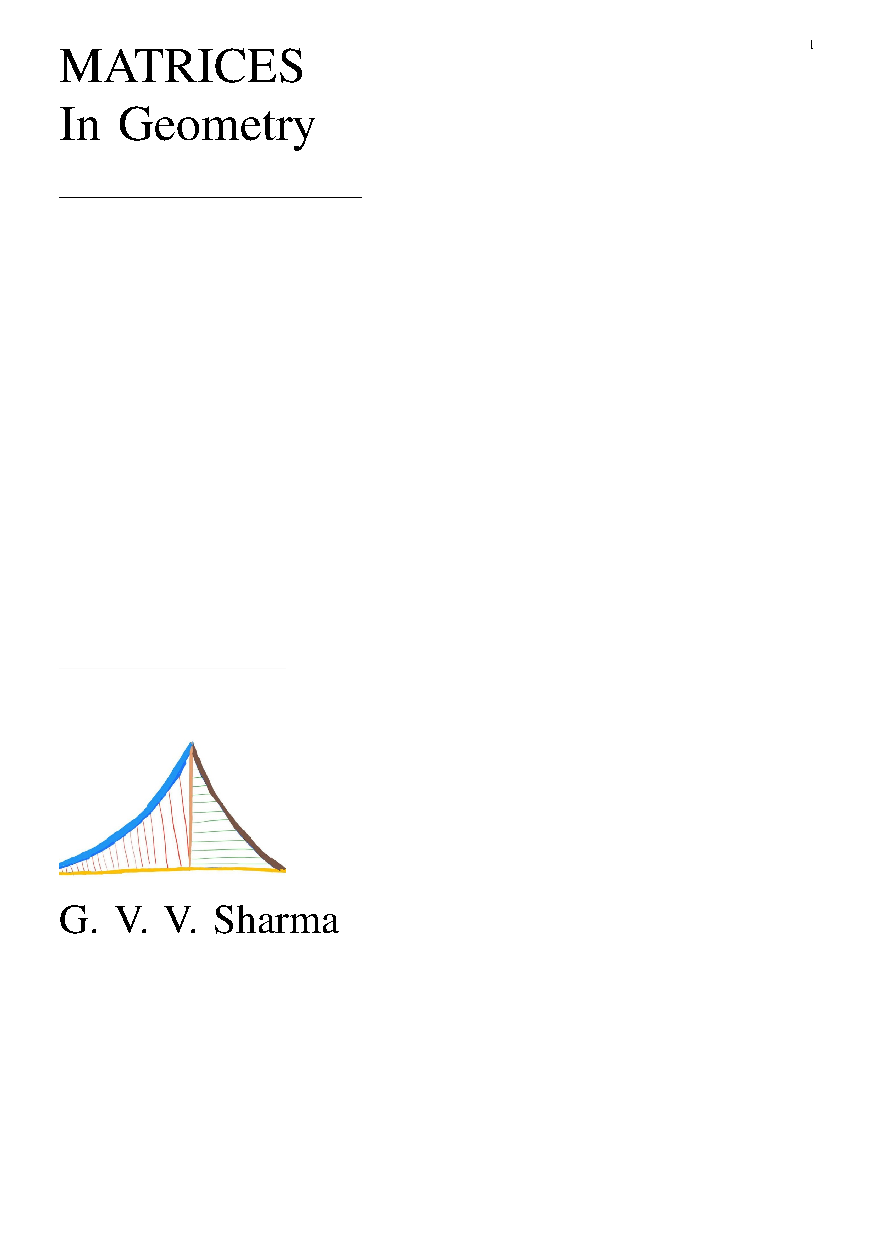
\includegraphics[width=0.75\columnwidth]{chapters/12/6/3/8/figs/main.png}
		\caption{}
		\label{fig:12/6/3/8}
  	\end{figure}
The equation of the conic can be represented as
\begin{align}
\vec{x}^{\top}\myvec{1&0\\0&0}\vec{x}+2\myvec{-2&\frac{-1}{2}}\vec{x}+4=0
\end{align}
So,
\begin{align}
\vec{V}=\myvec{1&0\\0&0},
\vec{u}^{\top}=\myvec{-2&\frac{-1}{2}},
f=4
\end{align}
The direction vector of the line passing through (2,0) and (4,4) is 
\begin{align}
\vec{m}=\myvec{1\\2}
\implies
\vec{n}=\myvec{2\\-1}.
\end{align}
The eigenvector corresponding to the zero eigenvalue is 
\begin{align}
\vec{p}_1=\myvec{0\\1},
\end{align}
In
\eqref{eq:conic_tangent_q_eigen},
\begin{align}
	\kappa=\frac{\myvec{0&1}\myvec{-2\\ \frac{-1}{2}}}{\myvec{0&1}\myvec{2\\-1}}
	=\frac{1}{2}
\end{align}
Substituting  $\kappa$,
from 
\eqref{eq:conic_tangent_q_eigen},
\begin{align}
	\myvec{\sbrak{\myvec{-2\\\frac{-1}{2}}+\frac{1}{2}\myvec{2\\-1}}^{\top} \\ \myvec{1&0\\0&0}}\vec{q} &= \myvec{-4 \\ \frac{1}{2}\myvec{2\\-1}-\myvec{-2\\\frac{-1}{2}}}\\
	\implies
	\myvec{-1&-1 \\ 1&0 \\ 0&0}\vec{q}&=\myvec{-4 \\ 3 \\ 0}
\end{align}
yielding
\begin{align}
\myvec{-1&-1 \\ 1&0}\vec{q} = \myvec{-4\\3}
\end{align}
The augmented matrix is 
\begin{align*}
  \myvec{
                -1&-1&\vrule&-4\\
	        1&0&\vrule&3}
  \xleftrightarrow[]{R_1 \leftarrow R_1+ 2R_2}
     \myvec{
	         1&-1&\vrule&2\\
	         1&0&\vrule&3}
      \\
 \xleftrightarrow[]{R_2 \leftarrow R_2 - R_1}
     \myvec{
	         1&-1&\vrule&2\\
	         0&1&\vrule&1}
 \xleftrightarrow[]{R_1 \leftarrow R_1 + R_2}
     \myvec{
	         1&0&\vrule&3\\
	         0&1&\vrule&1}
      \\ \implies \vec{q}=\myvec{3\\1}
\end{align*}
which is the desired 
point of contact.
See Fig. 
		\ref{fig:12/6/3/8}.



\iffalse
\latexprintindex
\fi

\end{document}


	\item Find the angles $A, B, C$ if 
%    \label{prop:angle2d}
  \begin{align}
    \label{eq:app-angle2d}
			\cos A \triangleq 
\frac{\brak{\vec{B}-\vec{A}}^{\top}{\vec{C}-\vec{A}}}{\norm{\vec{B}-\vec{A}}\norm{\vec{C}-\vec{A}}}
  \end{align}\\
  \solution
\begin{enumerate}
	\item From 
		\eqref{eq:app-geo-dir-vec-ab},
		\eqref{eq:app-geo-dir-vec-ca},
		\eqref{eq:app-geo-norm-ab}
		and
		\eqref{eq:app-geo-norm-ca}
\begin{align}
	(\vec{B}-\vec{A})^{\top}(\vec{C}-\vec{A})&=\myvec{-5&7}\myvec{-4\\-4}\\
	&=-8
	\\
	\implies
	\cos{A}&= \frac{-8}{\sqrt{74} \sqrt{32}}
	= \frac{-1}{\sqrt{37}}\\
	\implies A&=\cos^{-1}{\frac{-1}{\sqrt{37}}}
\end{align}
	\item From 
		\eqref{eq:app-geo-dir-vec-ab},
		\eqref{eq:app-geo-dir-vec-bc},
		\eqref{eq:app-geo-norm-ab}
		and
		\eqref{eq:app-geo-norm-bc}
\begin{align}
	(\vec{C}-\vec{B})^{\top}(\vec{A}-\vec{B})&=\myvec{1&-11}\myvec{5\\-7}\\
	&= 82
	\\
	\implies
	\cos{B}&= \frac{82}{\sqrt{74} \sqrt{122}}
	= \frac{41}{\sqrt{2257}}\\
	\implies B&=\cos^{-1}{\frac{41}{\sqrt{2257}}}
\end{align}
	\item From 
		\eqref{eq:app-geo-dir-vec-bc},
		\eqref{eq:app-geo-dir-vec-ca},
		\eqref{eq:app-geo-norm-bc}
		and
		\eqref{eq:app-geo-norm-ca}
\begin{align}
	(\vec{A}-\vec{C})^{\top}(\vec{B}-\vec{C})&=\myvec{4&4}\myvec{-1\\11}\\
	&=40
	\\
\implies	\cos{C}&= \frac{40}{\sqrt{32} \sqrt{122}}
	= \frac{5}{\sqrt{61}}\\
	\implies C&=\cos^{-1}{\frac{5}{\sqrt{61}}}
\end{align}

\end{enumerate}
%  	\documentclass[journal]{IEEEtran}
\usepackage{gvv-book}
\usepackage{gvv}
%\usepackage{styles/front}
%\usepackage{Wiley-AuthoringTemplate}
%\usepackage[sectionbib,authoryear]{natbib}% for name-date citation comment the below line
%\usepackage[sectionbib,numbers]{natbib}% for numbered citation comment the above line

%%********************************************************************%%
%%       How many levels of section head would you like numbered?     %%
%% 0= no section numbers, 1= section, 2= section, 3= subsection %%
\setcounter{secnumdepth}{3}
%%********************************************************************%%
%%**********************************************************************%%
%%     How many levels of section head would you like to appear in the  %%
%%				Table of Contents?			%%
%% 0= chapter, 1= section, 2= section, 3= subsection titles.	%%
\setcounter{tocdepth}{2}
%%**********************************************************************%%

%\includeonly{ch01}
\makeindex

\begin{document}
\bibliographystyle{IEEEtran}
\onecolumn


\title{
	\begin{flushleft}
	MATRICES \\ In Geometry
	\\
\rule{0.4\columnwidth}{0.4pt}
\end{flushleft}
}
\author{
\vspace{7cm}
	\begin{flushleft}
\includegraphics[width=0.2\columnwidth]{figs/logo.jpg}
\\
		{	\huge G. V. V. Sharma}
		\\
\vspace{1cm}
https://creativecommons.org/licenses/by-sa/3.0/
\\
and
\\
https://www.gnu.org/licenses/fdl-1.3.en.html
	\end{flushleft}
%\IEEEpubid{\makebox[\columnwidth]{978-1-7281-5966-1/20/\$31.00 ©2020 IEEE \hfill} \hspace{\columnsep}\makebox[\columnwidth]{ }}
}
\maketitle

\newpage


\tableofcontents

\newpage
\twocolumn

%\section{Triangle}
\section{Vectors}
Consider a triangle with vertices
		\begin{align}
			\label{eq:tri-pts}
			\vec{A} = \myvec{1 \\ -1},\,
			\vec{B} = \myvec{-4 \\ 6},\,
			\vec{C} = \myvec{-3 \\ -5}
		\end{align}
\subsection{Sides}
%\renewcommand{\theequation}{\theenumi}
\begin{enumerate}[label=\thesubsection.\arabic*.,ref=\thesubsection.\theenumi]
%\numberwithin{equation}{enumi}
\item The direction vector of $AB$ is defined as
		\begin{align}
			\vec{B}-
			\vec{A}
		\end{align}
Find the direction vectors of $AB, BC$ and $CA$.
\\
\solution 
\begin{enumerate} 
\item  The Direction vector of $AB$ is 
	\begin{align}  \vec{B} - \vec{A} 
		=\myvec{ -4\\ 6 } - \myvec{ 1\\ -1 }
 = \myvec{ -4 - 1\\ 6 - (-1) } = \myvec{ -5\\ 7 }
		\label{eq:app-geo-dir-vec-ab}
 \end{align}
\item The Direction vector of $BC$ is
	\begin{align} \vec{C} - \vec{B}=\myvec{ -3\\ -5} - \myvec{ -4\\ 6 }
 = \myvec{ -3 - (-4)\\ -5 - 6 } = \myvec{1\\ -11 }
		\label{eq:app-geo-dir-vec-bc}
  \end{align}
  \item  The Direction vector of $CA$  is
	  \begin{align}  \vec{A} - \vec{C} =\myvec{ 1\\ -1 }-\myvec{ -3\\ -5}
 = \myvec{ 1 - (-3)\\ -1 - (-5) } = \myvec{ 4\\ 4 }
		\label{eq:app-geo-dir-vec-ca}
  \end{align}
 \end{enumerate}
%	\input{solutions/1/1/1/prob_1.tex}
	\item The length of side $BC$ is 
		\label{prob:side-length}
		\begin{align}
			c = \norm{\vec{B}-\vec{A}} \triangleq \sqrt{\brak{\vec{B}-\vec{A}}^{\top}\brak{\vec{B}-\vec{A}}}
		\end{align}
		where
		\begin{align}
			\vec{A}^{\top}\triangleq\myvec{1 & -1}
		\end{align}
		Similarly, 
		\begin{align}
b = \norm{\vec{C}-\vec{B}},\,
a = \norm{\vec{A}-\vec{C}}
		\end{align}
		Find $a, b, c$.
\begin{enumerate}
	\item 
	From 	
		\eqref{eq:app-geo-dir-vec-ab},
\begin{align}
\vec{A}-\vec{B} &= \myvec{5\\-7}, \\
\implies 	c &= 	\norm{\vec{B}-\vec{A}} = \norm{\vec{A}-\vec{B}} 
	\\
	&= \sqrt{\myvec{5 & -7}\myvec{5\\-7}}
= \sqrt{\brak{5}^2 +\brak{7}^2}\\
	&=\sqrt{74}
		\label{eq:app-geo-norm-ab}
\end{align}
	\item Similarly, from 
		\eqref{eq:app-geo-dir-vec-bc},
\begin{align}
	a &= \norm{\vec{B}-\vec{C}} 
	= \sqrt{\myvec{-1 & 11}\myvec{-1\\11}}
\\
&= \sqrt{\brak{1}^2+\brak{11}^2}
	= \sqrt{122}
		\label{eq:app-geo-norm-bc}
\end{align}
and
		from 		\eqref{eq:app-geo-dir-vec-ca},
	\item 
		\begin{align}
			b &= \norm{\vec{A}-\vec{C}} = \sqrt{\myvec{4 & 4}\myvec{4\\4}}
\\
&= \sqrt{\brak{4}^2+\brak{4}^2}
	=\sqrt{32}
		\label{eq:app-geo-norm-ca}
\end{align}
\end{enumerate}
%  \\            
  %\input{solutions/1/1/2a/main.tex}
\item   Points $\vec{A}, \vec{B}, \vec{C}$ are defined to be collinear if 
		\begin{align}
			\label{eq:app-app-line-rank}
			\rank{\myvec{1 & 1 & 1 \\ \vec{A}& \vec{B}&\vec{C}}} = 2
		\end{align}
Are the given points in
			\eqref{eq:app-tri-pts}
collinear?
\\
\solution 
From 
			\eqref{eq:app-tri-pts},
\begin{align}
    \label{eq:app-1.1.3,2}
\myvec{
    1 & 1 & 1\\
    \vec{A} & \vec{B} & \vec{C} \\
    } 
    =
    %\label{eq:app-matthrowoperations}
    \myvec{
    1 & 1 & 1
    \\
    1 & -4 & -3
    \\
    -1 & 6 & -5
    }
     \xleftrightarrow[]{R_3 \leftarrow R_3+R_2}
    \myvec{
    1 & 1 & 1
    \\
    1 & -4 & -3
    \\
    0 & 2 & -8 
    }
    \\
     \xleftrightarrow[]{R_2\leftarrow R_1-R_2}
    \myvec{
    1 & 1 & 1
    \\
    0 & 5 & 4
    \\
    0 & 2 & -8 
    }
     \xleftrightarrow[]{R_3\leftarrow R_3-\frac{2}{5}R_2}
    \myvec{
    1 & 1 & 1
    \\
    0 & 5 & 4
    \\
    0 & 0 & \frac{-48}{5}
    }
\end{align}
There are no zero rows. So,
\begin{align}
    \text{rank}\myvec{
    1 & 1 & 1\\
    \vec{A} & \vec{B} & \vec{C} \\
    } &= 3 
\end{align}  
Hence,  the points $\vec{A},\vec{B},\vec{C}$ are not collinear. 
This is visible in 
\figref{fig1:Triangle}.
\begin{figure}[H]
\centering
\includegraphics[width=0.75\columnwidth]{figs/triangle/vector.pdf}
\caption{$\triangle ABC$}
\label{fig1:Triangle}
\end{figure}
% \\		\input{solutions/1/1/3/main.tex}
\item The parameteric form of the equation  of $AB$ is 
		\begin{align}
			\label{eq:app-geo-param}
			\vec{x}=\vec{A}+k\vec{m} \quad k \ne 0,
		\end{align}
		where
		\begin{align}
\vec{m}=\vec{B}-\vec{A}
		\end{align}
is the direction vector of $AB$.
Find the parameteric equations of $AB, BC$ and $CA$.
\\
\solution
From 
			\eqref{eq:app-geo-param} and
		\eqref{eq:app-geo-dir-vec-ab},
the parametric equation for $AB$ is given by
\begin{align}
AB: \vec{x} = &\myvec{1\\-1} + k \myvec{-5\\7}
\end{align}
Similarly, from 
		\eqref{eq:app-geo-dir-vec-bc} and
		\eqref{eq:app-geo-dir-vec-ca},
\begin{align}
BC: \vec{x} = &\myvec{-4\\6} + k \myvec{1\\-11}\\
CA: \vec{x} = &\myvec{-3\\-5} + k \myvec{4\\4}
\end{align}

%		\input{solutions/1/1/4/main.tex}
\item The normal form of the equation of $AB$  is 
		\begin{align}
			\label{eq:app-geo-normal}
			\vec{n}^{\top}\brak{	\vec{x}-\vec{A}} = 0
		\end{align}
		where 
		\begin{align}
			\vec{n}^{\top}\vec{m}&=\vec{n}^{\top}\brak{\vec{B}-\vec{A}} = 0
			\\
			\text{or, } \vec{n}&=\myvec{0 & 1 \\ -1 & 0} \vec{m}
			\label{eq:app-geo-norm-vec}
		\end{align}
Find the normal form of the equations of $AB, BC$ and $CA$.
\\
\solution
\begin{enumerate}
	\item
From
		\eqref{eq:app-geo-dir-vec-bc}, 
the direction vector of side $\vec{BC}$ is
\begin{align}
\vec{m}
	&=\myvec{1\\-11}
	\\
\implies \vec{n} &= \myvec{0 & 1\\
  -1 & 0}\myvec{1\\-11}
 = \myvec{-11\\-1}
		\label{eq:app-geo-norm-vec-bc}
\end{align}
from 
			\eqref{eq:app-geo-norm-vec}.
Hence, from 
			\eqref{eq:app-geo-normal},
the normal equation of side $BC$ is 
\begin{align}
	\vec{n}^{\top}\brak{	\vec{x}-\vec{B}} &= 0
			\\
\implies    \myvec{-11 & -1}\vec{x}&=\myvec{-11 & -1}\myvec{-4\\6}\\
    \implies
BC: \quad    \myvec{11 & 1}\vec{x}&=-38
\end{align}
\item Similarly, for $AB$,
from 
		\eqref{eq:app-geo-dir-vec-ab}, 
\begin{align}
	\vec{m} &= \myvec{-5\\7}
	\\
\implies        \vec{n} 
                &= \myvec{0&1\\-1&0}\myvec{-5\\7}
                = \myvec{7\\5}
		\label{eq:app-geo-norm-vec-ab}
\end{align}
and 
\begin{align}
	\vec{n}^{\top}\brak{	\vec{x}-\vec{A}} &= 0
	\\
	\implies
                AB: \quad  \vec{n}^{\top}\vec{x} &= \myvec{7&5}\myvec{1\\-1}\\    
       \implies\myvec{7&5}\vec{x} &= 2
\end{align}
\item For 
$CA$, 
from 
		\eqref{eq:app-geo-dir-vec-ca}, 
\begin{align}
\vec{m} &= \myvec{1 \\ 1}
\\
		\label{eq:app-geo-norm-vec-ca}
\implies \vec{n} 
&= \myvec{0&1 \\ -1&0}\myvec{1 \\ 1}
= \myvec{1 \\ -1}\\
\\
\implies	\vec{n}^{\top}\brak{	\vec{x}-\vec{C}} &= 0
\\
\implies \myvec{1&-1}{\vec{x}} &= \myvec{1&-1}\myvec{-3 \\ -5} 
= 2 
\end{align}
\end{enumerate}

%\input{solutions/1/1/5/assign1.tex}
\item The area of $\triangle ABC$ is defined as
		\begin{align}
			\label{eq:app-tri-area-cross}
			\frac{1}{2}\norm{{\brak{\vec{A}-\vec{B}}\times \brak{\vec{A}-\vec{C}}}}
		\end{align}
		where
		\begin{align}
			\vec{A}\times\vec{B} \triangleq \mydet{1 & -4 \\-1 & 6}
		\end{align}
		Find the area of $\triangle ABC$.\\
\solution
From
		\eqref{eq:app-geo-dir-vec-ab}
		and
		\eqref{eq:app-geo-dir-vec-ca},
\begin{align}
	\vec{A}-\vec{B}=\myvec{5\\-7},
	\vec{A}-\vec{C}&=\myvec{4\\4}\\
\implies (\vec{A}-\vec{B})\times(\vec{A}-\vec{C}) &=\mydet{5 & 4\\-7 & 4}\\
&=5\times 4-4\times (-7)\\&=48\\
\implies\frac{1}{2}\norm{(\vec{A}-\vec{B})\times(\vec{A}-\vec{C})}&=\frac{48}{2}=24
\end{align}
which is the desired area.

%  		\input{solutions/1/1/6/main.tex}
	\item Find the angles $A, B, C$ if 
%    \label{prop:angle2d}
  \begin{align}
    \label{eq:app-angle2d}
			\cos A \triangleq 
\frac{\brak{\vec{B}-\vec{A}}^{\top}{\vec{C}-\vec{A}}}{\norm{\vec{B}-\vec{A}}\norm{\vec{C}-\vec{A}}}
  \end{align}\\
  \solution
\begin{enumerate}
	\item From 
		\eqref{eq:app-geo-dir-vec-ab},
		\eqref{eq:app-geo-dir-vec-ca},
		\eqref{eq:app-geo-norm-ab}
		and
		\eqref{eq:app-geo-norm-ca}
\begin{align}
	(\vec{B}-\vec{A})^{\top}(\vec{C}-\vec{A})&=\myvec{-5&7}\myvec{-4\\-4}\\
	&=-8
	\\
	\implies
	\cos{A}&= \frac{-8}{\sqrt{74} \sqrt{32}}
	= \frac{-1}{\sqrt{37}}\\
	\implies A&=\cos^{-1}{\frac{-1}{\sqrt{37}}}
\end{align}
	\item From 
		\eqref{eq:app-geo-dir-vec-ab},
		\eqref{eq:app-geo-dir-vec-bc},
		\eqref{eq:app-geo-norm-ab}
		and
		\eqref{eq:app-geo-norm-bc}
\begin{align}
	(\vec{C}-\vec{B})^{\top}(\vec{A}-\vec{B})&=\myvec{1&-11}\myvec{5\\-7}\\
	&= 82
	\\
	\implies
	\cos{B}&= \frac{82}{\sqrt{74} \sqrt{122}}
	= \frac{41}{\sqrt{2257}}\\
	\implies B&=\cos^{-1}{\frac{41}{\sqrt{2257}}}
\end{align}
	\item From 
		\eqref{eq:app-geo-dir-vec-bc},
		\eqref{eq:app-geo-dir-vec-ca},
		\eqref{eq:app-geo-norm-bc}
		and
		\eqref{eq:app-geo-norm-ca}
\begin{align}
	(\vec{A}-\vec{C})^{\top}(\vec{B}-\vec{C})&=\myvec{4&4}\myvec{-1\\11}\\
	&=40
	\\
\implies	\cos{C}&= \frac{40}{\sqrt{32} \sqrt{122}}
	= \frac{5}{\sqrt{61}}\\
	\implies C&=\cos^{-1}{\frac{5}{\sqrt{61}}}
\end{align}

\end{enumerate}
%  	\input{solutions/1/1/7/main.tex}
All codes for this section are available at
\begin{lstlisting}
	codes/triangle/sides.py
\end{lstlisting}
\end{enumerate}

\subsection{Median}
\input{chapters/triangle/median}
\subsection{Altitude}
\input{chapters/triangle/altitude}
\subsection{Perpendicular Bisector}
\input{chapters/triangle/perp-bisect}
\subsection{Angle Bisector}
\input{chapters/triangle/angle-bisect}
\subsection{Eigenvalues and Eigenvectors}
\input{chapters/triangle/eigen}
\section{Matrices}
The mid point of $PB$ is
\begin{align}
\vec{M} =\frac{1}{2}(\vec{P}+\vec{B})
	= \myvec{4 \\ -2}  
\end{align}
which is equal to the direction vector of $OM$.
\begin{align}
\because \vec{M} \equiv
	 \myvec{1 \\ -\frac{1}{2}},
	m = -\frac{1}{2}
\end{align}
which is the desired slope.
See 
		\figref{fig:11/10/1/5}.
	\begin{figure}[!ht]
		\centering
 \includegraphics[width=\columnwidth]{chapters/11/10/1/5/figs/line.png}
		\caption{}
		\label{fig:11/10/1/5}
  	\end{figure}


%\section{Quadrilateral}
%\input{./chapters/exercises/quad_geo_exer}

\appendices
\section{Tangents to a Circle}
\numberwithin{equation}{section}
	\begin{figure}[H]
		\centering
 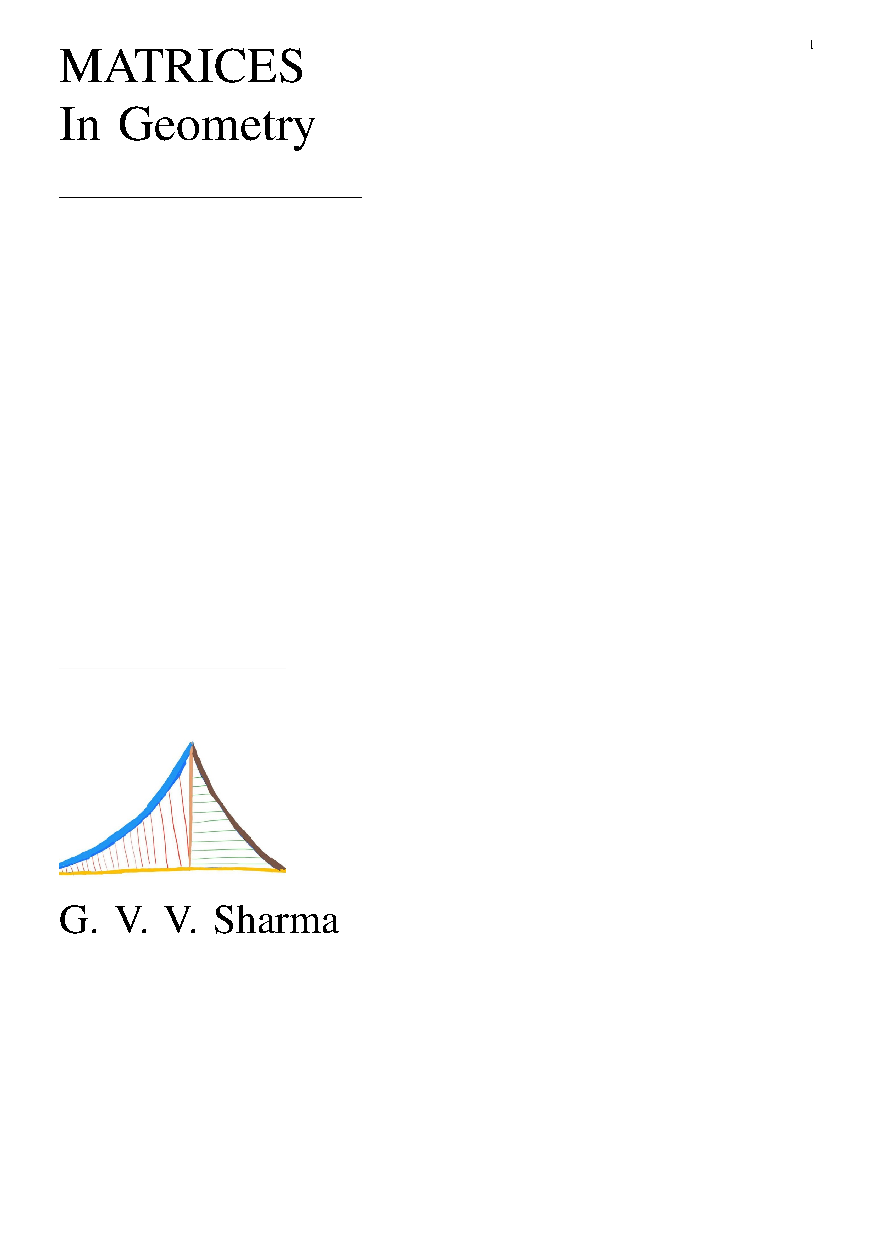
\includegraphics[width=0.75\columnwidth]{chapters/12/6/3/8/figs/main.png}
		\caption{}
		\label{fig:12/6/3/8}
  	\end{figure}
The equation of the conic can be represented as
\begin{align}
\vec{x}^{\top}\myvec{1&0\\0&0}\vec{x}+2\myvec{-2&\frac{-1}{2}}\vec{x}+4=0
\end{align}
So,
\begin{align}
\vec{V}=\myvec{1&0\\0&0},
\vec{u}^{\top}=\myvec{-2&\frac{-1}{2}},
f=4
\end{align}
The direction vector of the line passing through (2,0) and (4,4) is 
\begin{align}
\vec{m}=\myvec{1\\2}
\implies
\vec{n}=\myvec{2\\-1}.
\end{align}
The eigenvector corresponding to the zero eigenvalue is 
\begin{align}
\vec{p}_1=\myvec{0\\1},
\end{align}
In
\eqref{eq:conic_tangent_q_eigen},
\begin{align}
	\kappa=\frac{\myvec{0&1}\myvec{-2\\ \frac{-1}{2}}}{\myvec{0&1}\myvec{2\\-1}}
	=\frac{1}{2}
\end{align}
Substituting  $\kappa$,
from 
\eqref{eq:conic_tangent_q_eigen},
\begin{align}
	\myvec{\sbrak{\myvec{-2\\\frac{-1}{2}}+\frac{1}{2}\myvec{2\\-1}}^{\top} \\ \myvec{1&0\\0&0}}\vec{q} &= \myvec{-4 \\ \frac{1}{2}\myvec{2\\-1}-\myvec{-2\\\frac{-1}{2}}}\\
	\implies
	\myvec{-1&-1 \\ 1&0 \\ 0&0}\vec{q}&=\myvec{-4 \\ 3 \\ 0}
\end{align}
yielding
\begin{align}
\myvec{-1&-1 \\ 1&0}\vec{q} = \myvec{-4\\3}
\end{align}
The augmented matrix is 
\begin{align*}
  \myvec{
                -1&-1&\vrule&-4\\
	        1&0&\vrule&3}
  \xleftrightarrow[]{R_1 \leftarrow R_1+ 2R_2}
     \myvec{
	         1&-1&\vrule&2\\
	         1&0&\vrule&3}
      \\
 \xleftrightarrow[]{R_2 \leftarrow R_2 - R_1}
     \myvec{
	         1&-1&\vrule&2\\
	         0&1&\vrule&1}
 \xleftrightarrow[]{R_1 \leftarrow R_1 + R_2}
     \myvec{
	         1&0&\vrule&3\\
	         0&1&\vrule&1}
      \\ \implies \vec{q}=\myvec{3\\1}
\end{align*}
which is the desired 
point of contact.
See Fig. 
		\ref{fig:12/6/3/8}.



\iffalse
\latexprintindex
\fi

\end{document}


All codes for this section are available at
\begin{lstlisting}
	codes/triangle/sides.py
\end{lstlisting}
\end{enumerate}

\newpage
\subsection{Median}
\input{chapters/triangle/median}
\newpage
\subsection{Altitude}
\input{chapters/triangle/altitude}
\newpage
\subsection{Perpendicular Bisector}
\input{chapters/triangle/perp-bisect}
\newpage
\subsection{Angle Bisector}
\input{chapters/triangle/angle-bisect}
\newpage
\subsection{Eigenvalues and Eigenvectors}
\input{chapters/triangle/eigen}
\newpage
\subsection{Addition and Subtraction}
\begin{enumerate}[label=\thesubsection.\arabic*,ref=\thesubsection.\theenumi]
\item Find the sum of the vectors $\vec{a}=\hat{i}-2\hat{j}+\hat{k}$, $\vec{b}=-2\hat{i}+4\hat{j}+5\hat{k}$ and $\vec{c}=\hat{i}-6\hat{j}-7\hat{k}$.
\item 

	In triangle ABC 
		(\figref{fig:chapters/12/10/2/18/}),
		which of the following is not true:
 \begin{enumerate}
         \item $\overrightarrow{AB}+\overrightarrow{BC}+\overrightarrow{CA}$=$\vec{0}$
         \item $\overrightarrow{AB}+\overrightarrow{BC}-\overrightarrow{CA}$=$\vec{0}$
         \item $\overrightarrow{AB}+\overrightarrow{BC}-\overrightarrow{CA}$=$\vec{0}$
         \item $\overrightarrow{AB}-\overrightarrow{BC}+\overrightarrow{CA}$=$\vec{0}$
\end{enumerate}
\begin{figure}[!ht]
\centering
\includegraphics[width = \columnwidth]{./chapters/12/10/2/18/figs/triangle.png}
\caption{}
	\label{fig:chapters/12/10/2/18/}
\end{figure}
\solution
		\begin{align}
	\overrightarrow{AB}+\overrightarrow{BC}+\overrightarrow{CA} &=
\vec{B}-\vec{A} + \vec{C} - \vec{B} + \vec{A} - \vec{C}
= 0
\\
	\overrightarrow{AB}+\overrightarrow{BC}-\overrightarrow{AC} &=
\vec{B}-\vec{A} + \vec{C} - \vec{B} - (\vec{C} - \vec{A})
= 0
\\
	\overrightarrow{AB}+\overrightarrow{BC}+\overrightarrow{AC} &=
\vec{B}-\vec{A} + \vec{C} - \vec{B} + \vec{C} - \vec{A}
= 2(\vec{C}-\vec{A})
\\
	\overrightarrow{AB}-\overrightarrow{CB}+\overrightarrow{CA} &=
\vec{B}-\vec{A} - (\vec{B} - \vec{C}) + \vec{A} - \vec{C}
= 0
\end{align}

\item A girl walks 4 km towards west, then she walks 3 km in a direction 30$^{\circ}$ east of north and stops. Determine the girl's displacement from her initial point of departure.\\
	\solution
		See  
\figref{fig:chapters/12/10/5/3Fig1}.
Let the initial position
be
\begin{align}
	\vec{A}=\myvec{0\\0}
\end{align}
After going west, the position becomes
\begin{align}
			\vec{B}=\myvec{-4\\0}
\end{align}
If the final position be $\vec{C}$, from the given information,
\begin{align}
	 \vec{C}-\vec{B}=3\myvec{\cos{60\degree}\\\sin{60\degree}}
	 \implies 
	\vec{C}  
=\myvec{-\frac{5}{2}\\[2pt] \frac{3\sqrt{3}}{2}}
\end{align}
which is the desired displacement. 
\begin{figure}[H] 
 \begin{center} 
 \includegraphics[width=0.75\columnwidth]{chapters/12/10/5/3/figs/fig.pdf} 
 \end{center} 
\caption{} 
\label{fig:chapters/12/10/5/3Fig1} 
\end{figure}

\item Without using distance formula, show that points A(– 2, – 1), B(4, 0), C(3, 3) and D(–3, 2) are the vertices of a parallelogram.
\label{chapters/11/10/1/9}
\\
\solution
	  From \eqref{eq:two-pgm},
\begin{align}
\vec{A}-\vec{B} = 
\vec{D}-\vec{C} =  \myvec{-6\\-1}
\end{align}
Hence, $ABCD$ is a parallelogram.
See \figref{fig:chapters/11/10/1/91}.
\begin{figure}[H]
  \centering
   %\includegraphics[width=0.75\columnwidth]{chapters/11/10/1/9/figs/paralellogram.png}
   \includegraphics[width=0.75\columnwidth]{chapters/11/10/1/9/figs/fig.pdf}
    \caption{}
     \label{fig:chapters/11/10/1/91}  
\end{figure}




\item The fourth vertex $\vec{D}$ of a parallelogram $\vec{ABCD}$ whose three vertices are
	$\vec{A} (–2, 3), \vec{B} (6, 7)\text { and } \vec{C} (8, 3)$ is
\begin{enumerate}
	\item $(0, 1)$
	\item $(0, –1)$
	\item $ (–1,0)$
	\item$(1, 0)$
\end{enumerate}
\item Points $\vec{A}(4,3), \vec{B}(6,4),\vec{C}(5,-6)$  and  $\vec{D}(-3,5)$ are the vertices of a parallelogram.
\end{enumerate}

\newpage
\subsection{Section Formula}
See  
\figref{fig:chapters/10/7/4/6Fig1}.
\begin{figure}[H]
 \begin{center}
 \includegraphics[width=0.75\columnwidth]{chapters/10/7/4/6/figs/fig.pdf}
 \end{center}
\caption{}
\label{fig:chapters/10/7/4/6Fig1}
\end{figure}
	Using section formula
	  \eqref{eq:section_formula},
\begin{align}
\vec{D} =\frac{3\vec{A}+\vec{B}}{4}
	=\frac{1}{4}\myvec{13\\ 23}
	\\
\vec{E} =\frac{3\vec{A}+\vec{C}}{4}
	=\frac{1}{4}\myvec{19\\ 20}
	\\
	\vec{A}- \vec{D} 
	=\frac{1}{4}\myvec{3\\ 1},\,
	  \vec{A}- \vec{E}  
	=\frac{1}{4}\myvec{-3\\ 1}
	\\
	\vec{A}- \vec{B} =\myvec{3\\1},
	  \vec{B}-\vec{C} =\myvec{-6\\3}
\end{align}
yielding
\begin{align}
ar(ABD) =\frac{1}{2} \norm{\brak{\vec{A}-\vec{D}}  \times 
   \brak{\vec{A}- \vec{E}}} 
	=	\frac{15}{32}
	\\
	  ar(ABC) =\frac{1}{2} \norm{\brak{\vec{A}-\vec{B}}  \times 
   \brak{\vec{B}- \vec{C}}} 
	=	\frac{15}{2}
	\\
	\implies \frac{ar\brak{ADE}}{ar\brak{ABC}}=\frac{1}{16}
\end{align}

\subsection{Rank}
\begin{enumerate}[label=\thesubsection.\arabic*,ref=\thesubsection.\theenumi]
\item Determine if the points $(1,5),(2,3)$ and $(-2,-11)$ are collinear.
	\\
	\solution
Use		\eqref{prop:lin-dep-rank}.
%		\begin{enumerate}[label=\thesubsection.\arabic*, ref=\thesubsection.\theenumi]
    \item The value of $m$ which makes the points $(0,0)$, $(2m, -4)$, and $(3,6)$ collinear, is \underline{\hspace{1cm}}.
    \hfill (10, 2022)
		\item If $\vec{A}(1, 2)$, $\vec{O}(0, 0)$, and $\vec{C}(a, 6)$ are collinear, then the value of $a$ is
		\hfill (10, 2021)
	\item Show that the points $A(-2\hat{i} + 3\hat{j} + 5\hat{k})$, $B(\hat{i} + 2\hat{j} + 3\hat{k})$, and $C(7\hat{i} - \hat{k})$ are collinear. \hfill (12, 2019)
	\item Using vectors, prove that the points $(2, -1, 3)$, $(3, -5, 1)$, and $(-1, 11, 9)$ are collinear. \hfill (12, 2019)
\item Find the value of $p$ for which the points $(-5, 1)$, $(1, p)$, and $(4, -2)$ are collinear. \hfill (10, 2019)
\item Find a relation between $x$ and $y$ if the points $A(x, y)$, $B(-4, 6)$, and $C(-2, 3)$ are collinear. \hfill (10, 2019)
\item For what value of $p$ are the points $(2, 1)$, $(p, -1)$, and $(-1, 3)$ collinear? \hfill (10, 2019)
\end{enumerate}

\item Show that the points $\vec{A}(1,2,7), \vec{B}(2,6,3)$ and $\vec{C}(3,10,-1)$ are collinear.
	\\
	\solution
%		\begin{enumerate}[label=\thesubsection.\arabic*, ref=\thesubsection.\theenumi]
    \item The value of $m$ which makes the points $(0,0)$, $(2m, -4)$, and $(3,6)$ collinear, is \underline{\hspace{1cm}}.
    \hfill (10, 2022)
		\item If $\vec{A}(1, 2)$, $\vec{O}(0, 0)$, and $\vec{C}(a, 6)$ are collinear, then the value of $a$ is
		\hfill (10, 2021)
	\item Show that the points $A(-2\hat{i} + 3\hat{j} + 5\hat{k})$, $B(\hat{i} + 2\hat{j} + 3\hat{k})$, and $C(7\hat{i} - \hat{k})$ are collinear. \hfill (12, 2019)
	\item Using vectors, prove that the points $(2, -1, 3)$, $(3, -5, 1)$, and $(-1, 11, 9)$ are collinear. \hfill (12, 2019)
\item Find the value of $p$ for which the points $(-5, 1)$, $(1, p)$, and $(4, -2)$ are collinear. \hfill (10, 2019)
\item Find a relation between $x$ and $y$ if the points $A(x, y)$, $B(-4, 6)$, and $C(-2, 3)$ are collinear. \hfill (10, 2019)
\item For what value of $p$ are the points $(2, 1)$, $(p, -1)$, and $(-1, 3)$ collinear? \hfill (10, 2019)
\end{enumerate}

\item Show that the vectors $2\hat{i}-3\hat{j}+4\hat{k}$ and $-4\hat{i}+6\hat{j}-8\hat{k}$ are collinear.
   \\ 
    \solution 
%		\begin{enumerate}[label=\thesubsection.\arabic*, ref=\thesubsection.\theenumi]
    \item The value of $m$ which makes the points $(0,0)$, $(2m, -4)$, and $(3,6)$ collinear, is \underline{\hspace{1cm}}.
    \hfill (10, 2022)
		\item If $\vec{A}(1, 2)$, $\vec{O}(0, 0)$, and $\vec{C}(a, 6)$ are collinear, then the value of $a$ is
		\hfill (10, 2021)
	\item Show that the points $A(-2\hat{i} + 3\hat{j} + 5\hat{k})$, $B(\hat{i} + 2\hat{j} + 3\hat{k})$, and $C(7\hat{i} - \hat{k})$ are collinear. \hfill (12, 2019)
	\item Using vectors, prove that the points $(2, -1, 3)$, $(3, -5, 1)$, and $(-1, 11, 9)$ are collinear. \hfill (12, 2019)
\item Find the value of $p$ for which the points $(-5, 1)$, $(1, p)$, and $(4, -2)$ are collinear. \hfill (10, 2019)
\item Find a relation between $x$ and $y$ if the points $A(x, y)$, $B(-4, 6)$, and $C(-2, 3)$ are collinear. \hfill (10, 2019)
\item For what value of $p$ are the points $(2, 1)$, $(p, -1)$, and $(-1, 3)$ collinear? \hfill (10, 2019)
\end{enumerate}

\item Show that the points (2, 3, 4), (–1, –2, 1), (5, 8, 7) are collinear.
		\\
		\solution
	%	\begin{enumerate}[label=\thesubsection.\arabic*, ref=\thesubsection.\theenumi]
    \item The value of $m$ which makes the points $(0,0)$, $(2m, -4)$, and $(3,6)$ collinear, is \underline{\hspace{1cm}}.
    \hfill (10, 2022)
		\item If $\vec{A}(1, 2)$, $\vec{O}(0, 0)$, and $\vec{C}(a, 6)$ are collinear, then the value of $a$ is
		\hfill (10, 2021)
	\item Show that the points $A(-2\hat{i} + 3\hat{j} + 5\hat{k})$, $B(\hat{i} + 2\hat{j} + 3\hat{k})$, and $C(7\hat{i} - \hat{k})$ are collinear. \hfill (12, 2019)
	\item Using vectors, prove that the points $(2, -1, 3)$, $(3, -5, 1)$, and $(-1, 11, 9)$ are collinear. \hfill (12, 2019)
\item Find the value of $p$ for which the points $(-5, 1)$, $(1, p)$, and $(4, -2)$ are collinear. \hfill (10, 2019)
\item Find a relation between $x$ and $y$ if the points $A(x, y)$, $B(-4, 6)$, and $C(-2, 3)$ are collinear. \hfill (10, 2019)
\item For what value of $p$ are the points $(2, 1)$, $(p, -1)$, and $(-1, 3)$ collinear? \hfill (10, 2019)
\end{enumerate}

\item In each of the following, find the value of '$k$', for which the points are collinear.
\begin{enumerate}
\item $(7, –2), (5, 1), (3, k)$
\item $(8, 1), (k, – 4), (2, –5)$
\end{enumerate}
		\label{10/7/3/2}
\solution
	%	\begin{enumerate}[label=\thesubsection.\arabic*, ref=\thesubsection.\theenumi]
    \item The value of $m$ which makes the points $(0,0)$, $(2m, -4)$, and $(3,6)$ collinear, is \underline{\hspace{1cm}}.
    \hfill (10, 2022)
		\item If $\vec{A}(1, 2)$, $\vec{O}(0, 0)$, and $\vec{C}(a, 6)$ are collinear, then the value of $a$ is
		\hfill (10, 2021)
	\item Show that the points $A(-2\hat{i} + 3\hat{j} + 5\hat{k})$, $B(\hat{i} + 2\hat{j} + 3\hat{k})$, and $C(7\hat{i} - \hat{k})$ are collinear. \hfill (12, 2019)
	\item Using vectors, prove that the points $(2, -1, 3)$, $(3, -5, 1)$, and $(-1, 11, 9)$ are collinear. \hfill (12, 2019)
\item Find the value of $p$ for which the points $(-5, 1)$, $(1, p)$, and $(4, -2)$ are collinear. \hfill (10, 2019)
\item Find a relation between $x$ and $y$ if the points $A(x, y)$, $B(-4, 6)$, and $C(-2, 3)$ are collinear. \hfill (10, 2019)
\item For what value of $p$ are the points $(2, 1)$, $(p, -1)$, and $(-1, 3)$ collinear? \hfill (10, 2019)
\end{enumerate}

\item Find a relation between $x$ and $y$ if the points $(x, y), (1, 2)$  and  $(7, 0)$ are collinear.
\\
\solution
	%\begin{enumerate}[label=\thesubsection.\arabic*, ref=\thesubsection.\theenumi]
    \item The value of $m$ which makes the points $(0,0)$, $(2m, -4)$, and $(3,6)$ collinear, is \underline{\hspace{1cm}}.
    \hfill (10, 2022)
		\item If $\vec{A}(1, 2)$, $\vec{O}(0, 0)$, and $\vec{C}(a, 6)$ are collinear, then the value of $a$ is
		\hfill (10, 2021)
	\item Show that the points $A(-2\hat{i} + 3\hat{j} + 5\hat{k})$, $B(\hat{i} + 2\hat{j} + 3\hat{k})$, and $C(7\hat{i} - \hat{k})$ are collinear. \hfill (12, 2019)
	\item Using vectors, prove that the points $(2, -1, 3)$, $(3, -5, 1)$, and $(-1, 11, 9)$ are collinear. \hfill (12, 2019)
\item Find the value of $p$ for which the points $(-5, 1)$, $(1, p)$, and $(4, -2)$ are collinear. \hfill (10, 2019)
\item Find a relation between $x$ and $y$ if the points $A(x, y)$, $B(-4, 6)$, and $C(-2, 3)$ are collinear. \hfill (10, 2019)
\item For what value of $p$ are the points $(2, 1)$, $(p, -1)$, and $(-1, 3)$ collinear? \hfill (10, 2019)
\end{enumerate}

\item If three points $(x, -1), (2, 1)$ and $(4, 5)$ are collinear, find the value of $x$.
\label{chapters/11/10/1/8}
%The mid point of $PB$ is
\begin{align}
\vec{M} =\frac{1}{2}(\vec{P}+\vec{B})
	= \myvec{4 \\ -2}  
\end{align}
which is equal to the direction vector of $OM$.
\begin{align}
\because \vec{M} \equiv
	 \myvec{1 \\ -\frac{1}{2}},
	m = -\frac{1}{2}
\end{align}
which is the desired slope.
See 
		\figref{fig:11/10/1/5}.
	\begin{figure}[!ht]
		\centering
 \includegraphics[width=\columnwidth]{chapters/11/10/1/5/figs/line.png}
		\caption{}
		\label{fig:11/10/1/5}
  	\end{figure}

\item If three points $(h, 0), (a, b)$ and $(0, k)$ lie on a line, 
show that 
\begin{align}
\frac{a}{h}+\frac{b}{k}=1
\end{align}
\label{chapters/11/10/1/13}
%The mid point of $PB$ is
\begin{align}
\vec{M} =\frac{1}{2}(\vec{P}+\vec{B})
	= \myvec{4 \\ -2}  
\end{align}
which is equal to the direction vector of $OM$.
\begin{align}
\because \vec{M} \equiv
	 \myvec{1 \\ -\frac{1}{2}},
	m = -\frac{1}{2}
\end{align}
which is the desired slope.
See 
		\figref{fig:11/10/1/5}.
	\begin{figure}[!ht]
		\centering
 \includegraphics[width=\columnwidth]{chapters/11/10/1/5/figs/line.png}
		\caption{}
		\label{fig:11/10/1/5}
  	\end{figure}

\item Show that the points A (1, -2, -8), B (5, 0, -2) and C (11, 3, 7) are collinear, and find the ratio in which B divides AC.\\
\item lf the points $\vec{A}(1,2),\vec{0}(0,0)\text{ and }\vec{C}(a,b)$ are collinear,then
\begin{enumerate}
\item a=b
\item a=2b
\item 2a=b
\item a=-b
\end{enumerate}
\end{enumerate}
True/false
\begin{enumerate}[label=\thesection.\arabic*,ref=\thesection.\theenumi,resume*]
	\item $\triangle\vec{A}\vec{B}\vec{C}$ with vertices $\vec{A}(-2,0), \vec{B}(2,0) \text{ and }\vec{C}(0,2)$ is similar to $\triangle \vec{DEF}$  with vertices $\vec {D}(-4,0),\vec{E}(4,0)  \text{ and } \vec{F}(0,4)$  
	\item Point $ (-4,2)$ lies on the line segment joining the points $ \vec{A}(-4,6) \text{ and } \vec{B}(-4,-6)$
 \item The points $(0,5),(0,-9)\text{ and }(3,6)$ are collinear
\item Points $\vec{A}(3,1), \vec{B}(12,-2) \text{ and } \vec {C}(0,2)$ cannot be the vertices of a triangle
\item Find the value of $m$ if the points $(5,1),(-2,-3) \text{ and }(8,2m)$ are collinear.
\item Find the values of k if the points $\vec{A}(k+1,2k),\vec{B}(3k,2k+3)\text{ and }\vec{C}(5k-1,5k)$ are collinear
\item Using vectors, find the value of $k$ such that the points $(k,-10,3)$, $(1,-1,3)$ $\text{ and }$ $(3,5,3)$ are collinear.
\end{enumerate}

\subsection{Length}
\begin{enumerate}[label=\thesection.\arabic*,ref=\thesection.\theenumi]
\item Compute the magnitude of the following vectors:
\begin{align}
	\vec{a}&=\hat{i}+\hat{j}+\hat{k}
	\\
	\vec{b}&=2\hat{i}-7\hat{j}-3\hat{k}
	\\
	\vec{c}&=\frac{1}{\sqrt{3}}\hat{i}+\frac{1}{\sqrt{3}}\hat{j}-\frac{1}{3}\hat{k}
\end{align}
    \solution 
		Let 
\begin{align}
	\vec{a} = \myvec{1\\1\\1} , \vec{b} = \myvec{2\\ -7 \\ 3}, 
\vec{c} = \myvec{\dfrac{1}{\sqrt{3}}\\[2ex] \dfrac{1}{\sqrt{3}} \\[2ex] -\dfrac{1}{\sqrt{3}}} 
\label{eq:chapters/12/10/2/1/1}
\end{align}
Then
\begin{align}
	{\vec{a}^{\top}\vec{a}} &= \myvec{1  &  1  &  1}\myvec{1\\1\\1} = 3
\\
\implies 
	\norm{\vec{a}}&=\sqrt{3}, 
	\label{eq:chapters/12/10/2/1/3}
\end{align}
		from \eqref{eq:side-length}. Similarly,
\begin{align}
	\norm{\vec{b}}&=\sqrt{\vec{b}^{\top}\vec{b}}= \sqrt{62}, 
	\label{eq:chapters/12/10/2/1/4}
	\\ \norm{\vec{c}}&=\sqrt{\vec{c}^{\top}\vec{c}}	
=1
	\label{eq:chapters/12/10/2/1/5}
\end{align}




\item Find the value of x for which $x(\hat{i}+\hat{j}+\hat{k})$ is a unit vector.\\
	\solution
		\begin{align} 
\because
\vec{x}=x\myvec{1\\1\\1},
\norm{\vec{x}}=1
\implies 
x\sqrt{3}=1
\\
	\text{or, }x=\frac{1}{\sqrt{3}}
\end{align}   

\item If $\vec{a}=\vec{b}+\vec{c}$, then is it true that $|\vec{a}|=|\vec{b}|+|\vec{c}|$? Justify your answer.\\
	\solution
		Let 
\begin{align}
	\vec{a} = \myvec{1\\1\\1} , \vec{b} = \myvec{2\\ -7 \\ 3}, 
\vec{c} = \myvec{\dfrac{1}{\sqrt{3}}\\[2ex] \dfrac{1}{\sqrt{3}} \\[2ex] -\dfrac{1}{\sqrt{3}}} 
\label{eq:chapters/12/10/2/1/1}
\end{align}
Then
\begin{align}
	{\vec{a}^{\top}\vec{a}} &= \myvec{1  &  1  &  1}\myvec{1\\1\\1} = 3
\\
\implies 
	\norm{\vec{a}}&=\sqrt{3}, 
	\label{eq:chapters/12/10/2/1/3}
\end{align}
		from \eqref{eq:side-length}. Similarly,
\begin{align}
	\norm{\vec{b}}&=\sqrt{\vec{b}^{\top}\vec{b}}= \sqrt{62}, 
	\label{eq:chapters/12/10/2/1/4}
	\\ \norm{\vec{c}}&=\sqrt{\vec{c}^{\top}\vec{c}}	
=1
	\label{eq:chapters/12/10/2/1/5}
\end{align}




\item If $\overrightarrow {a}$ is a nonzero vector of magnitude `a' and $\lambda$ a nonzero scalar, then $\lambda\overrightarrow {a}$ is a unit vector if
\begin{enumerate} 
\item $\lambda=1$ 
\item $\lambda=-1$
\item $a=\abs{\lambda}$
\item $a=1/\abs{\lambda}$  
\end{enumerate}

\end{enumerate}

%
\newpage
\subsection{Direction}
\begin{enumerate}[label=\thesection.\arabic*,ref=\thesection.\theenumi]
\item For given vectors, $\vec{a}=2\hat{i}-\hat{j}+2\hat{k}$ and $\vec{b}=-\hat{i}+\hat{j}-\hat{k}$ , find the unit vector in the
direction of the vector $\vec{a}+\vec{b}$.
        \label{prob:12/10/2/9}
\\
    \solution 
		\begin{align}
	\because \vec a + \vec b = \myvec{ 2\\-1\\2 } + \myvec{ -1\\1\\-1 },
= \myvec{ 1\\0\\1 },
\\
	\norm{\vec a + \vec b } = \sqrt{2}
	\\
	\implies \frac{\vec a + \vec b }{\norm{\vec a + \vec b }} = \frac{1}{\sqrt{2}}\myvec{ 1\\0\\1 }
\end{align}
which, from  \eqref{eq:unit-vec} is the desired the unit vector.
		





\item Find a vector in the direction of vector $5\hat{i}-\hat{j}+2\hat{k}$ which has magnitude 8 units.
        \label{prob:12/10/2/10const}
   \\ 
    \solution 
		Let the required vector be 
    \begin{align}
c\myvec{5\\-1\\2}.
    \end{align}
    From the given information, 
    \begin{align}
        \norm{c\myvec{5\\-1\\2\\}} =  8 \\
	    \implies \abs{c} = \frac{4\sqrt{30}}{15}
        \label{eq:12/10/2/10const}
    \end{align}


\item Find the unit vector in the direction of the vector $\vec{a}=\hat{i}+\hat{j}+2\hat{k}$.
\item Find the unit vector in the direction of vector $\overrightarrow{PQ}$ , where $\vec{P}$ and $\vec{Q}$ are the points
(1, 2, 3) and (4, 5, 6), respectively.
	\item 
Find a vector of magnitude 5 units, and parallel to the resultant of the vectors $\vec{a} = 2\hat{i}+3\hat{j}-\hat{k}$ and $\vec{b} = \hat{i}-2\hat{j}+\hat{k}$.
\\
\solution
		\begin{align}
\because     \Vec{a}=\myvec{
        2\\3\\-1
    },\Vec{b}=\myvec{
        1\\-2\\1
    }\\
	\vec{a}+\vec{b}=\myvec{
        3\\1\\0
    }
    \implies
	\norm{\vec{a}+\vec{b}}=\sqrt{10}
\end{align}
From problem
        \ref{prob:12/10/2/9},
the unit vector in the direction of 
${\vec{a}+\vec{b}}$
is
\begin{align}
	\frac{{\vec{a}+\vec{b}}}{\norm{\vec{a}+\vec{b}}}
=\frac{1}{\sqrt{10}}\myvec{
        3\\1\\0
    }
\end{align}
The desired vector can then be expressed as
\begin{align}
\pm\frac{5}{\sqrt{10}}\myvec{
        3\\1\\0
    }
\end{align}


\item Find the direction cosines of the vector joining the points $\vec{A}$ (1, 2, –3) and
$\vec{B}$(–1, –2, 1), directed from $\vec{A}$ to $\vec{B}$.
	\\
    \solution 
		The unit vector  in the direction of AB is 
\begin{align}
	\frac{\vec{B}-\vec{A}}{\norm{\vec{B}-\vec{A}}}
	= \frac{1}{3}{\myvec{-1\\-2\\2}}
\end{align}
and the direction cosines are the elements of the above vector.

\item Show that the vector $\hat{i}+\hat{j}+\hat{k}$ is equally inclined to the axes OX, OY and OZ.
	\\
\solution
		Since all entries of the given vector 
\begin{align}
\myvec{1\\1\\1}
\end{align}
are equal, it is equally inclined to the axes.

\item If a line has the direction ratios –18, 12, –4, then what are its direction cosines?
		\\
		\solution
		Let
\begin{align}
	\vec{A} =\myvec{-18\\12\\-4}
\end{align}
Then the unit direction vector of the line is
\begin{align}
		\frac{\vec{A}}{\norm{\vec{A}}} =
\myvec{\frac{-9}{11}\\[2pt] \frac{6}{11}\\[2pt] \frac{-2}{11}}
\end{align}

	\item Find the direction cosines of the sides of a triangle whose vertices are $\myvec{3\\ 5\\-4 }$, $\myvec{ -1\\1 \\2 }$ and $\myvec{-5 \\-5 \\-2 }$.
		\\
		\solution
		Let the vertices be
\begin{align}
\vec{A} = \myvec{3\\5\\-4},
\vec{B} = \myvec{-1\\1\\2},
\vec{C} = \myvec{-5\\-5\\-2}
\end{align}
%
The direction vectors of the sides are,
\begin{align}
\vec{A} - \vec{B} = \myvec{4\\4\\-6} = \vec{m_1},
\vec{B} - \vec{C} = \myvec{4\\6\\4} = \vec{m_2}, 
\\
\vec{C} - \vec{A} = \myvec{-8\\-10\\2} =\vec{m_3},
\end{align}
%
The corresponding unit vectors are then obtained as
\begin{align}
 \myvec{ \frac{2}{\sqrt{17}} \\[1pt] \frac{2}{\sqrt{17}} \\[1pt] \frac{-3}{\sqrt{17}} },
 \myvec{ \frac{2}{\sqrt{17}} \\[1pt] \frac{3}{\sqrt{17}} \\[1pt] \frac{2}{\sqrt{17}} }, 
 \myvec{ \frac{-4}{\sqrt{42}} \\[1pt] \frac{-5}{\sqrt{42}} \\[1pt] \frac{1}{\sqrt{42}} } 
\end{align}

\item Find the direction cosines of the vector $\hat{i}+2\hat{j}+3\hat{k}$.
	\\
    \solution 
		The unit vector in the direction of the given vector is 
\begin{align}
	\vec{A} =\frac{1}{\sqrt{14}}\myvec{1\\2\\3}
\end{align}

    \item Find the direction cosines of a line which makes equal angles with the coordinate
    axes.
		\\
		\solution
		Let $\alpha$ be the angle made by the line with the axes.  The unit direction vector can be expressed as
    \begin{align}
	    \vec{x} &= \myvec{\cos\alpha\\\cos\alpha\\\cos\alpha} 
	\implies
	    \norm{\vec{x}}  = 1
	\\
	    \text{or, }\cos\alpha &= \frac{1}{\sqrt{3}}
    \end{align}
    Thus the unit direction vector  of the given line is 
    \begin{align}
	    \vec{x} = \frac{1}{\sqrt{3}} \myvec{1 \\ 1 \\ 1} 
\end{align}
    

\item Write down a unit vector in XY-plane, making an angle of 30$^{\circ}$ with the positive direction of x-axis.\\
\end{enumerate}

\newpage
\subsection{Scalar Product}
\begin{enumerate}[label=\thesubsection.\arabic*, ref=\thesubsection.\theenumi]
\item The angle between the vectors $\hat{i} - \hat{j}$ and $\hat{j} - \hat{k}$ is \rule{1cm}{0.2pt}.
\hfill (12, 2020)
\item Find the angle between unit vectors $\overrightarrow{a}$ and $\overrightarrow{b}$ so that $\sqrt{3}\overrightarrow{a}$ - $\overrightarrow{b}$ is also a unit vector.
\hfill (12, 2020)
    \item If $\overrightarrow{a}, \overrightarrow{b}, \overrightarrow{c}$ are three non-zero unequal vectors such that $\overrightarrow{a} \cdot \overrightarrow{b} = \overrightarrow{a} \cdot \overrightarrow{c}$, then find the angle between $\overrightarrow{a}$ and $\overrightarrow{b} - \overrightarrow{c}$.
    \hfill (12, 2023)
    \item $\overrightarrow{a}$ and $\overrightarrow{b}$ are two unit vectors such that
    \begin{align}
        \left| 2\overrightarrow{a} + 3\overrightarrow{b} \right| = \left| 3\overrightarrow{a} - 2\overrightarrow{b} \right|.
    \end{align}
  Find the angle between $\overrightarrow{a}$ and $\overrightarrow{b}$.
    \hfill (12, 2023)
	\item Find the angle between the line $\overrightarrow{r} = \hat{i} - \hat{j} + \hat{k} + \lambda (3\hat{i} - \hat{j} + 2\hat{k})$ and the plane $\overrightarrow{r} \cdot (\hat{i} + \hat{j} + \hat{k}) = 3$.

		\hfill (12, 2019)
\item Find the magnitude of each of the vectors $\overrightarrow{\vec{a}}$ and $\overrightarrow{\vec{b}}$, having the same magnitude such that the angle between them is $60\degree$ and their scalar product is $\frac{9}{2}$. \hfill (12, 2018)
\item Find the acute angle between the planes $\vec{r}\cdot\brak{ \hat{i}-\hat{2j}-\hat{2k}}=1$ and $\vec{r}\cdot \brak{\hat{3i}-\hat{6j}+\hat{2k}}=0$

\hfill (12, 2018)
\item If $\hat{i}+\hat{j}+{k} ,  2\hat{i}+5\hat{j} ,  3\hat{i}+2\hat{j}-3{k} ,  \hat{i}-6\hat{j}-{k}$ respectively are the position vectors of points A, B, C and D, then find the angle between the straight lines AB and CD. Find whether $\overrightarrow{AB}$ and $\overrightarrow{CD}$ are collinear or not. 
\hfill (12, 2018) 
\item If vectors $\overrightarrow{a}$ and $\overrightarrow{b}$ are such that
      $\abs{\overrightarrow{a}} = \frac{1}{2}$, $\abs{\overrightarrow{b}} = \frac{4}{\sqrt{3}}$
      and $\abs{\overrightarrow{a} \times \overrightarrow{b}} = \frac{1}{\sqrt{3}}$, then find
      $\abs{\overrightarrow{a}\cdot \overrightarrow{b} }$. \hfill (12, 2016)
\item If $\overrightarrow{a}$ and $\overrightarrow{b}$ are unit vectors, then what is the angle between
      $\overrightarrow{a}$ and $\overrightarrow{b}$ for $\overrightarrow{a} - \sqrt{2}\overrightarrow{b}$ to be a unit vector? \hfill (12, 2016)
\item Find the acute angle between the planes
      $  \overrightarrow{r} \cdot \brak{\hat{i}-2\hat{j}-2\hat{k}} = 1$
      and
      $  \overrightarrow{r} \cdot \brak{3\hat{i}-6\hat{j}+2\hat{k}} = 0$.
    \hfill (12, 2019)                                                    


\end{enumerate}

\newpage
\subsection{Orthogonality}
\begin{enumerate}[label=\thesubsection.\arabic*, ref=\thesubsection.\theenumi]
\item Show that the points \brak{7, 10}, \brak{-2, 5} and \brak{3, 4} are vertices of an isosceles right triangle.
The points form an isosceles right triangle.
\hfill (10, 2020)
    \item The points $(-4,0)$, $(4,0)$, and $(0,3)$ are the vertices of a:
    \begin{enumerate}
        \item right triangle
        \item isosceles triangle
        \item equilateral triangle
        \item scalene triangle
    \end{enumerate}
    \hfill (10, 2023)
    \item Show that the points $(-2,3)$, $(8,3)$, and $(6,7)$ are the vertices of a right-angled triangle.
    \hfill (10, 2023)
    \item If
    \begin{align}
        \overrightarrow{a} = 2\hat{i} + y\hat{j} + \hat{k}
    \end{align}
    and
    \begin{align}
        \overrightarrow{b} = \hat{i} + 2\hat{j} + 3\hat{k}
    \end{align}
    are two vectors for which the vector $(\overrightarrow{a} + \overrightarrow{b})$ is perpendicular to the vector $(\overrightarrow{a} - \overrightarrow{b})$, then find all the possible values of $y$.
    \hfill (12, 2023)
    \item Write the projection of the vector $(\overrightarrow{b} + \overrightarrow{c})$ on the vector $\overrightarrow{a}$, where
    \begin{align}
        \overrightarrow{a} = 2\hat{i} - 2\hat{j} + \hat{k},
    \end{align}
    \begin{align}
        \overrightarrow{b} = \hat{i} + 2\hat{j} - 2\hat{k},
    \end{align}
    and
    \begin{align}
        \overrightarrow{c} = 2\hat{i} - \hat{j} + 4\hat{k}.
    \end{align}
    \hfill (12, 2023)

    \item If
    \begin{align}
        \overrightarrow{a} = 2\hat{i} - \hat{j} + \hat{k},
    \end{align}
    \begin{align}
        \overrightarrow{b} = \hat{i} + \hat{j} - 2\hat{k},
    \end{align}
    and
    \begin{align}
        \overrightarrow{c} = \hat{i} + 3\hat{j} - \hat{k},
    \end{align}
    and the projection of vector $\overrightarrow{c} + \lambda \overrightarrow{b}$ on vector $\overrightarrow{a}$ is $2\sqrt{6}$, find the value of $\lambda$.
    \hfill (12, 2023)
    \item If
    \begin{align}
        \overrightarrow{a} = 2\hat{i} - \hat{j} + 2\hat{k},
    \end{align}
    and
    \begin{align}
        \overrightarrow{b} = 5\hat{i} - 3\hat{j} - 4\hat{k},
    \end{align}
    then find the ratio of the projection of vector $\overrightarrow{a}$ on vector $\overrightarrow{b}$ to the projection of vector $\overrightarrow{b}$ on vector $\overrightarrow{a}$.
    \hfill (12, 2023)

    \item Show that the three vectors $2\hat{i} - \hat{j} + \hat{k}$, $\hat{i} - 3\hat{j} - 5\hat{k}$, and $3\hat{i} - 4\hat{j} - 4\hat{k}$ form the vertices of a right-angled triangle. 
    \hfill (12, 2023)
    \item If
    \begin{align}
        \overrightarrow{a} = 2\hat{i} + 2\hat{j} + 3\hat{k},
    \end{align}
    \begin{align}
        \overrightarrow{b} = -\hat{i} + 2\hat{j} + \hat{k},
    \end{align}
    and
    \begin{align}
        \overrightarrow{c} = 3\hat{i} + \hat{j},
    \end{align}
    are such that the vector $(\overrightarrow{a} + \lambda \overrightarrow{b})$ is perpendicular to vector $\overrightarrow{c}$, then find the value of $\lambda$.
    \hfill (12, 2023)
		\item What kind of triangle is formed with vertices $\vec{A}(0, 2)$, $\vec{B}(-3, 0)$, and $\vec{C}(3, 0)$?
		\hfill (10, 2021)
		\begin{enumerate}
			\item A right triangle
			\item An equilateral triangle
			\item An isosceles triangle
			\item A scalene triangle
		\end{enumerate}
		\item Check whether the points $\vec{P}(5, -2)$, $\vec{Q}(6, 4)$, and $\vec{R}(7, -2)$ are the vertices of an isosceles triangle $\triangle PQR$. \hfill (10, 2021)
		\item The points $\vec{A}(0, 3)$, $\vec{B}(-2, a)$, and $\vec{C}(-1, 4)$ are the vertices of a right triangle, right-angled at $\vec{A}$. Find the value of $a$. \hfill (10, 2021)
	\item If $\vec{a} = 2\hat{i} - \hat{j} + 2\hat{k}$ and $\vec{b} = 5\hat{i} - 3\hat{j} - 4\hat{k}$, then find the ratio $\frac{\text{projection of vector } \vec{a} \text{ on } \vec{b}}{\text{projection of vector } \vec{b} \text{ on vector } \vec{a}}$. \hfill (12, 2021)
	\item Let $\hat{a}$ and $\hat{b}$ be two unit vectors. If the vectors $\vec{c} = \hat{a} + 2\hat{b}$ and $\vec{d} = 5\hat{a} - 4\hat{b}$ are perpendicular to each other, then find the angle between the vectors $\hat{a}$ and $\hat{b}$. \hfill (12, 2021)
%	
	\item Show that $\abs{\vec{a}} \vec{b} + \abs{\vec{b}} \vec{a}$ is perpendicular to $\abs{\vec{a}} \vec{b} - \abs{\vec{b}} \vec{a}$, for any two non-zero vectors $\vec{a}$ and $\vec{b}$. \hfill (12, 2021)
	\item Find the value of $p$ for which the following lines are perpendicular:
	\begin{align*}
	\dfrac{1-x}{3} = \dfrac{2y-14}{2p} = \dfrac{z-3}{2}; \quad \dfrac{1-x}{3p} = \dfrac{y-5}{1} = \dfrac{6-z}{5}.
	\end{align*} \hfill (12, 2019)
%	
	\item Show that the vectors $\hat{i} - 2\hat{j} + 3\hat{k}$, $-2\hat{i} + 3\hat{j} - 4\hat{k}$, and $\hat{i} - 3\hat{j} + 5\hat{k}$ are coplanar. \hfill (12, 2019)
	\item Find a unit vector perpendicular to both the vectors $\overrightarrow{a}$ and $\overrightarrow{b}$, where $\overrightarrow{a} = \hat{i} - 7\hat{j} + 7\hat{k}$ and $\overrightarrow{b} = 3\hat{i} - 2\hat{j} + 2\hat{k}$. \hfill (12, 2019)
	\item Let $\overrightarrow{a} = \hat{i} + 2\hat{j} - 3\hat{k}$ and $\overrightarrow{b} = 3\hat{i} - \hat{j} + 2\hat{k}$. Show that the vectors $\overrightarrow{a} + \overrightarrow{b}$ and $\overrightarrow{a} - \overrightarrow{b}$ are perpendicular to each other. \hfill (12, 2019)
\item Show that the vectors $\hat{i} - 2\hat{j} + 3\hat{k}$, $2\hat{i} + 3\hat{j} - 4\hat{k}$, and $\hat{i} - 3\hat{j} + 5\hat{k}$ are coplanar. \hfill (12, 2018)
\item Find the value of $P$ for which the following lines are perpendicular:
\begin{align*}
\frac{1 - x}{3} &= \frac{2y - 14}{2P} = \frac{z - 3}{2}
\end{align*}
\begin{align*}
\frac{1 - x}{3P} &= \frac{y - 5}{1} = \frac{6 - z}{5}
\end{align*}
\hfill (12, 2018)
\item Find the value of $x$ such that the four points with position vectors $\mathbf{A}(3\hat{i} + 2\hat{j} + \hat{k})$, $\mathbf{B}(4\hat{i} + x\hat{j} + 5\hat{k})$, $\mathbf{C}(4\hat{i} + 2\hat{j} - 2\hat{k})$, and $\mathbf{D}(6\hat{i} + 5\hat{j} - \hat{k})$ are coplanar. \hfill (12, 2018)
 \item Let $\overrightarrow{a}$, $\overrightarrow{b} $ and $\overrightarrow{c}$ be three vectors such that $\abs{\overrightarrow{a}}=1$, $\abs {\overrightarrow{b}}=2 $ and $\abs{\overrightarrow{c}}=3$. If the projection of $\overrightarrow{b}$ along $\overrightarrow{a}$ is equal to the projection of $\overrightarrow{c}$ along $\overrightarrow{a}$ ; and $\overrightarrow{b}$, $\overrightarrow{c}$ are perpendicular to each other, then find $\abs{3\overrightarrow{a}- 2\overrightarrow{b} +2\overrightarrow{c}}$.
\hfill (12, 2018)
\item Find the value of $P$ for which the following lines are perpendicular:
 \begin{align*}
 \frac{1-x}{3}=\frac{2y-14}{2p}=\frac{z-3}{2}; \frac{1-x}{3p}=\frac{y-5}{1}=\frac{6-z}{5}
 \end{align*}
 \hfill (12, 2018)
\item Find the value of $x$, for which the four points $\mathbf{A}\brak{x,1,-1}$, $\mathbf{B}\brak{4,5,1}$, $\mathbf{C}\brak{3,9,4}$ and $\mathbf{D}\brak{-4,4,4}$ are coplanar.
\hfill (12, 2018)
\item Let $\vec{a}=\hat{i}+\hat{2j}-\hat{3k}$ and $\vec{b}=\hat{3i}-\hat{j}+\hat{2k}$ be two vectors. Show that the vectors $(\vec{a}+\vec{b})$ and $(\vec{a}-\vec{b})$ are perpendicular to each other.
\hfill (12, 2018)
\item Using vectors, find the value of $x$ such that the four points $\mathbf{A}$ $\brak{x,5,-1}$,$\mathbf{B}$ $\brak{3,2,1}$,$\mathbf{C}$ $\brak{4,5,5}$ and $\mathbf{D}$ $\brak{4,2,-2}$ are coplanar.

\hfill (12, 2018) 
\item Find the angle between the line $\overrightarrow{r}=\brak{2\hat{i}-\hat{j}+3\hat{k}}+\lambda\brak{3\hat{i}-\hat{j}+2\hat{k}}$ and the plane $\overrightarrow{r}.\brak{\hat{i}+\hat{j}+\hat{k}}=3$.

\hfill (12, 2018) 
\item If $\abs{\overrightarrow{a}}=2$, $\abs{\overrightarrow{b}}=7$ and  $\overrightarrow{a}$ $X$ $\overrightarrow{b} =\hat{3i}+\hat{2j}+\hat{6k}$, find the angle between $\overrightarrow{a}$ and $\overrightarrow{b}$.
\hfill (12, 2018) 
    \item If $\vec{a} = 2\hat{i} - \hat{j} - 2\hat{k}$ and $\vec{b} = 7\hat{i} + 2\hat{j} - 3\hat{k}$, then express $\vec{b}$ in the form $\vec{b} = \vec{b_1} + \vec{b_2}$, where $\vec{b_1}$ is parallel to $\vec{a}$ and $\vec{b_2}$ is perpendicular to $\vec{a}$. \hfill (12, 2017)
    \item Prove that the points $\myvec{3,0}$, $\myvec{6,4}$, and $\myvec{-1,3}$ are the vertices of a right-angled isosceles triangle. \hfill (10, 2016)
\item Write the number of vectors of unit length perpendicular to both the vector
      \begin{align*}
          \vec{a} & = 2 \hat{i} + \hat{j} +2\hat{k} \quad\text{ and} \\
          \vec{b} & = \hat{j}+\hat{k}.
      \end{align*} \hfill (12, 2016)
\item Find the projection of the vector $\vec{a}=2\vec{i}+3\vec{j}+2\vec{k}$ on the vector $\vec{b}=2\vec{i}+2\vec{j}+\vec{k}$. \hfill (12, 2015)
\item The points $\vec{A}\brak{4, 7}$, $\vec{B}\brak{p, 3}$ and $\vec{C}\brak{7, 3}$ are the vertices of a right triangle, right-angled at $\vec{B}$. Find the value of $p$. \hfill (10, 2015)
\item If the two lines
\begin{align}
      L_1 : x=5,\frac{y}{3-\alpha}=\frac{z}{-2}\\
     L_2 : x=2,\frac{y}{-1}=\frac{z}{z-\alpha} 
   \end{align}
are perpendicular, then the value of $\alpha$ 
\hfill (12, 2021)
    \item If two vertices of an equilateral triangle are $(3,0)$ and $(6,0)$, find the third vertex.   
\hfill (10, 2011)
\item Show that the points $\brak{7, 10}$, $\brak{-2, 5}$ and $\brak{3, 4}$ are vertices of an isosceles right triangle.
\hfill (10, 2020)
\end{enumerate}

\newpage
\subsection{Vector Product}
\begin{enumerate}[label=\thesubsection.\arabic*,ref=\thesubsection.\theenumi]
		\item Find $\abs{\overrightarrow{a}\times\overrightarrow{b}},\text{ if }\overrightarrow{a}=\hat{i}-7\hat{j}+7\hat{k}\text{ and } \overrightarrow{b}=3\hat{i}-2\hat{j}+2\hat{k}$.
	\\
		\solution
		  From \eqref{eq:cross3d-submat},
\begin{align}
	\mydet{\vec{A}_{23}&\vec{B}_{23}}=\mydet{-7 & -2 \\ 7 & 2}=0\\
	\mydet{\vec{A}_{31}&\vec{B}_{31}}=\mydet{1 & 3 \\ 7 & 2}=-19\\
	\mydet{\vec{A}_{12}&\vec{B}_{12}}=\mydet{1 & 3 \\ -7 & -2}=19,
	\\
	\norm{\vec{a}\times\vec{b}}
	 = \norm{\myvec{ \mydet{\vec{A}_{23} & \vec{B}_{23}} \\[1ex] \mydet{\vec{A}_{31} & \vec{B}_{31}} \\[1ex] \mydet{\vec{A}_{12}  & \vec{B}_{12}}}}
=19\sqrt{2}
\end{align}
from 
  \eqref{eq:cross3d}.

\item Find $\lambda$ and $\mu$ if $(2\hat{i}+6\hat{j}+27\hat{k})\times(\hat{i}+\lambda \hat{j} + \mu \hat{k})=\overrightarrow{0}$.
	\\
		\solution
		From 
		 Formula \ref{prop:lin-dep-cross},
performing row reduction, 
\begin{align}
 \myvec{2&6&27 \\ 1& \lambda & \mu}
	\xleftrightarrow{R_{2}\leftarrow 2R_{2}-R_{1}}  	
 \myvec{2&6&27 \\ 0& 2\lambda -6 & 2\mu-27}
\end{align}
For the above matrix to have rank 1,
\begin{align}
	\mu=\frac{27}{2},
	\lambda=3.
\end{align}


\item Find the area of the triangle with vertices $A(1, 1, 2), B(2, 3, 5)$ and $C(1, 5, 5)$.
	\\
		\solution
		\begin{align}
\because \vec{B}-\vec{A} = \myvec{1\\2\\3}, 
\vec{C}-\vec{A} = \myvec{0\\4\\3},
\\
	\frac{1}{2} \norm{\myvec{1\\2\\3} \times \myvec{0\\4\\3}} 
	= 	\frac{1}{2}\norm{\myvec{-6\\3\\4}}
= \frac{\sqrt{61}}{2}
\end{align}
			using 
        \eqref{eq:11/10/1/1area-diag}, 
which is the the desired area.






\item Find the area of the parallelogram whose adjacent sides are determined by the vectors $\overrightarrow{a}=\hat{i}-\hat{j}+3\hat{k}$ and $\overrightarrow{b}=2\hat{i}-7\hat{j}+\hat{k}$.
	\\
		\solution
					From \eqref{eq:tri-area-cross},
			the desired area is obtained as
\begin{align}
	\norm{\myvec{1\\-1\\3} \times \myvec{2\\ -7 \\ 1}}
	=\norm{\myvec{20\\5\\-5}}
= 15\sqrt{2}
\end{align}


\item Find the area of a rhombus if its vertices are $A(3,0), B(4,5), C(-1,4)$  and  $D(-2,-1)$ taken in order. 
	\\
		\solution
	The area of the rhombus is
\begin{align}
                \norm{\myvec{\vec{A-D}}\times \myvec{\vec{B-A}}}=\mydet{5 & 1\\1 & 5} = 24
\end{align}
See 
\figref{fig:chapters/10/7/2/10/gFig1}.
\begin{figure}[!h]
 \begin{center}
  \includegraphics[width=\columnwidth]{chapters/10/7/2/10/figs/fig.pdf}
 \end{center}
\caption{}
\label{fig:chapters/10/7/2/10/gFig1}
\end{figure}

\item Let the vectors $\overrightarrow{a}$ and $\overrightarrow{b}$ be such that $|\overrightarrow{a}| = 3$ and $|\overrightarrow{b}| = \dfrac{\sqrt{2}}{3}$, then $\overrightarrow{a} \times \overrightarrow{b}$ is a unit vector, if the angle between $\overrightarrow{a}$ and $\overrightarrow{b}$ is
\begin{enumerate}
\item $\frac{\pi}{6}$
\item $\frac{\pi}{4}$
\item $\frac{\pi}{3}$
\item $\frac{\pi}{2}$
\end{enumerate}
		\solution
		From the given information and 
	\eqref{eq:cross-sin}
%
\begin{align}
	\norm{\vec{a} \times \vec{b}} & = \norm{\vec{a}} \norm{\vec{b}} \sin \theta =1\\
\implies\sin \theta & = \frac{1} {\norm{\vec{a}} \norm{\vec{b}}}
 = \frac{1}{\sqrt{2}}\\
\implies\theta &= 
 \frac{\pi}{4} 
\end{align}

\item Area of a rectangle having vertices A, B, C and D with position vectors $ -\hat{i}+ \frac{1}{2} \hat{j}+4\hat{k}, \hat{i}+ \frac{1}{2} \hat{j}+4\hat{k}, \hat{i}-\frac{1}{2} \hat{j}+4\hat{k}$ and $-\hat{i}- \frac{1}{2} \hat{j}+4\hat{k}$, respectively is
\begin{enumerate}
\item $\frac{1}{2}$
\item 1
\item 2
\item 4
\end{enumerate}
		\solution
		Since
\begin{align}
\vec{A} - \vec{B} &= \myvec{-2\\0\\0}\\
\vec{C} -\vec{B} &= \myvec{0\\-1\\0}
\end{align}
area of the rectangle is
\begin{align}
 \norm{\brak{\vec{A} -\vec{B}} \times \brak{\vec{C}-\vec{D}}}
= 2
\end{align} 
\iffalse
See Fig. 
   \ref{fig:chapters/12/10/4/12Rect_ABCD}
\begin{figure}[H]
  \centering
   \includegraphics[width=0.75\columnwidth]{chapters/12/10/4/12/figs/Figure_1.png}
   \caption{}
   \label{fig:chapters/12/10/4/12Rect_ABCD}
\end{figure}
\fi





\item Find the area of the triangle whose vertices are 
\begin{enumerate}
\item $(2, 3), (–1, 0), (2, – 4)$
\item $(–5, –1), (3, –5), (5, 2)$ 
\end{enumerate}
		\label{10/7/3/1}
\solution
		    See \tabref{eq:10/7/3/1/area}.
\begin{table}[H]
    \centering
    \caption{}
    \label{eq:10/7/3/1/area}
    \begin{tabular}{|c|c|c|c|}
        \hline
	     & $\vec{A}-\vec{B}$  & $\vec{A}-\vec{C}$  & $\frac{1}{2}\|\brak{\vec{A}-\vec{B}} \times \brak{\vec{A}-\vec{C}}\|$ \\
        \hline
         a)& $\myvec{ 3 \\3 }$ & $\myvec{ 0 \\ 7 }$ & $\frac{21}{2}$ \\
        \hline
	    b)& $\myvec{
 -8 \\
 4 
 }$
         &$\myvec{
 -10 \\
 -3 
 }$
  &  $32$   \\
        \hline
    \end{tabular}
\end{table}


\item Find the area of the triangle formed by joining the mid-points of the sides of the triangle whose vertices are $A(0, –1), B(2, 1)$  and  $C(0, 3)$. Find the ratio of this area to the area of the given triangle.
	\\
\solution
		Using 
	  \eqref{eq:section_formula},
the mid point coordinates are given by
	\begin{align}
		\vec{P} = \frac{1}{2}\vec(\vec{A}+\vec{B})  = \myvec{1\\0}\\
		\vec{Q} = \frac{1}{2}\vec(\vec{B}+\vec{C}) = \myvec{1\\2}\\
		\vec{R} = \frac{1}{2}\vec(\vec{A}+\vec{C}) = \myvec{0\\1}
	\end{align}
	\begin{align}
\because		\vec{P}-\vec{Q} =  \myvec{
 0 \\
 -2 
 },\,
		\vec{Q}-\vec{R} =   \myvec{
 1 \\
 1 
 }
 \\
		ar(PQR)=\frac{1}{2}{\norm{\vec(\vec{P}-\vec{Q})\times\vec(\vec{Q}-\vec{R})}}
		=1
	\end{align}
	Similarly, 
	\begin{align}
		\vec{A}-\vec{B} = \myvec{
 -2 \\
 -2 
 }
 ,\,
		\vec{A}-\vec{C} =  \myvec{
 0 \\
 -4 
 }
 \\
 \implies
		ar(ABC)=\frac{1}{2}{\norm{\vec(\vec{A}-\vec{B})\times\vec(\vec{A}-\vec{C})}}
=4
\\
		\implies \frac{ar\brak{PQR}}{ar\brak{ABC}} = \frac{1}{4}
	\end{align}
	See 
\figref{fig:10/7/3/3Fig}
\begin{figure}[H]
	\begin{center} 
	    \includegraphics[width=0.75\columnwidth]{chapters/10/7/3/3/figs/fig.pdf}
	\end{center}
\caption{}
\label{fig:10/7/3/3Fig}
\end{figure}


\item Find the area of the quadrilateral whose vertices, taken in order, are $A(– 4, – 2), B(– 3, – 5), C(3, – 2)$  and $ D(2, 3)$.
	\\
\solution
		See 
\figref{fig:chapters/10/7/3/4/Fig1}
\begin{figure}[H]
 \begin{center}
  \includegraphics[width=0.75\columnwidth]{chapters/10/7/3/4/figs/fig.pdf}
 \end{center}
\caption{}
\label{fig:chapters/10/7/3/4/Fig1}
\end{figure}
\begin{align}
\because	\vec{A}- \vec{B} =\myvec{-1\\3},\,
	  \vec{A}- \vec{D} =\myvec{-6\\-5},
	  \\
	\vec{B}- \vec{C} =\myvec{-6\\-5},\,
	  \vec{B}- \vec{D} =\myvec{-3\\-8},
	  \\
	  ar(ABD)=\frac{1}{2} \norm{\brak{\vec{A}-\vec{B}}  \times 
   \brak{\vec{A}- \vec{D}}} 
	=	\frac{23}{2}
	\\
	  ar(BCD)=\frac{1}{2} \norm{\brak{\vec{B}-\vec{C}}  \times 
   \brak{\vec{B}- \vec{D}}} 
	=	\frac{33}{2}
	\\
\implies	ar(ABCD)=  ar(ABD) +  ar(BCD)
	= 28
\end{align}


\item Verify that a median of a triangle divides it into two triangles of equal areas for $\triangle ABC$ whose vertices are $\vec{A}(4, -6), \vec{B}(3, 2), \text{ and } \vec{C}(5, 2)$. 
		\label{10/7/3/5}
		\\
\solution
		\begin{align}
\vec{D}=\frac{\vec{B}+\vec{C}}{2}
=\myvec{4\\ 0},
\\
	\vec{A}- \vec{B} =\myvec{1\\ -4},\,
	  \vec{A}- \vec{D} =\myvec{0\\ -6}
	  \\
	  \implies
  ar(ABD)=\frac{1}{2} \norm{\brak{\vec{A}-\vec{B}}  \times 
   \brak{\vec{A}- \vec{D}}} 
	       =3	
	       \\
	\vec{A}- \vec{C} =\myvec{-1\\ -8},\,
	  \vec{A}- \vec{D} =\myvec{0\\ -6}
	  \\
	  \implies
  ar(ACD)=\frac{1}{2} \norm{\brak{\vec{A}-\vec{C}}  \times 
   \brak{\vec{A}- \vec{D}}} 
   \\
	= 3 =
ar(ABD)
\end{align}
See  
\figref{fig:10/7/3/5/}.
\begin{figure}[H]
\centering
\includegraphics[width=0.75\columnwidth]{chapters/10/7/3/5/figs/fig.pdf}
\caption{}
\label{fig:10/7/3/5/}
\end{figure} 

\item The two adjacent sides of a parallelogram are 
$\vec{a}= 2\hat{i}-4\hat{j}+5\hat{k}$  and  $\vec{b} =\hat{i}-2\hat{j}-3\hat{k}$.
Find the unit vector parallel to its diagonal. Also, find its area.\\
	\solution
		The diagonals of the parallelogram are given by
\begin{align}
 \vec{a} + \vec{b} = \myvec{3 \\-6\\2},\, 
 \vec{a} - \vec{b} = \myvec{1 \\-2\\8}
\end{align}
and the corresponding unit vectors are
\begin{align}
	\frac{\vec{a} + \vec{b}}{\norm{\vec{a} + \vec{b}}}  = \myvec{\frac{3}{\sqrt{45}}\\[1ex]-\frac{6}{\sqrt{45}}\\[1ex]\frac{2}{\sqrt{45}}},\, 
	\frac{\vec{a} - \vec{b}}{\norm{\vec{a} - \vec{b}}}  = \myvec{\frac{1}{\sqrt{69}}\\[1ex]-\frac{2}{\sqrt{69}}\\[1ex]\frac{8}{\sqrt{69}}}
\end{align}
%
The area of the parallelogram is given by
\begin{align}
	\norm{\vec{a}\times\vec{b}}  = \norm{\myvec{22 \\-11\\0}} = \sqrt{605}
\end{align}


\item The vertices of a $\triangle ABC$ are $\vec{A}(4,6), \vec{B}(1,5)$ and  $\vec{C}(7,2)$. A line is drawn to intersect sides $AB$ and $AC$ at $\vec{D}$ and $\vec{E}$ respectively, such that $\frac{AD}{AB} = \frac{AE}{AC} = \frac{1}{4}$. Calculate the area of $\triangle ADE$ and compare it with the area of the $\triangle ABC$.
\\
\solution
	See  
\figref{fig:chapters/10/7/4/6Fig1}.
\begin{figure}[H]
 \begin{center}
 \includegraphics[width=0.75\columnwidth]{chapters/10/7/4/6/figs/fig.pdf}
 \end{center}
\caption{}
\label{fig:chapters/10/7/4/6Fig1}
\end{figure}
	Using section formula
	  \eqref{eq:section_formula},
\begin{align}
\vec{D} =\frac{3\vec{A}+\vec{B}}{4}
	=\frac{1}{4}\myvec{13\\ 23}
	\\
\vec{E} =\frac{3\vec{A}+\vec{C}}{4}
	=\frac{1}{4}\myvec{19\\ 20}
	\\
	\vec{A}- \vec{D} 
	=\frac{1}{4}\myvec{3\\ 1},\,
	  \vec{A}- \vec{E}  
	=\frac{1}{4}\myvec{-3\\ 1}
	\\
	\vec{A}- \vec{B} =\myvec{3\\1},
	  \vec{B}-\vec{C} =\myvec{-6\\3}
\end{align}
yielding
\begin{align}
ar(ABD) =\frac{1}{2} \norm{\brak{\vec{A}-\vec{D}}  \times 
   \brak{\vec{A}- \vec{E}}} 
	=	\frac{15}{32}
	\\
	  ar(ABC) =\frac{1}{2} \norm{\brak{\vec{A}-\vec{B}}  \times 
   \brak{\vec{B}- \vec{C}}} 
	=	\frac{15}{2}
	\\
	\implies \frac{ar\brak{ADE}}{ar\brak{ABC}}=\frac{1}{16}
\end{align}

    \item Draw a quadrilateral in the Cartesian plane, whose vertices are 
    \begin{align}
        \vec{A} = \myvec{-4\\5},\, \vec{B} = \myvec{0\\7},\, 
        \vec{C} = \myvec{5\\-5},\, \vec{D} = \myvec{-4\\-2}.
    \end{align}
    Also, find its area.
\label{chapters/11/10/1/1}
   \\ 
    \solution 
See \figref{fig:11/10/1/1quad}.
    From 
        \eqref{eq:11/10/1/1area-diag},
    \begin{align}
ar\brak{ABCD}
	       = \frac{121}{2}
        \label{eq:11/10/1/1ans}
    \end{align}
    \begin{figure}[H]
        \centering
        \includegraphics[width=0.75\columnwidth]{chapters/11/10/1/1/figs/fig.pdf}
        \caption{Plot of quadrilateral $ABCD$}
        \label{fig:11/10/1/1quad}
    \end{figure}

\item Find the area of region bounded by the triangle whose
	vertices are $(1, 0), (2, 2) \text{ and } (3, 1)$. 
\item Find the area of region bounded by the triangle whose vertices
	are $(– 1, 0), (1, 3) \text{ and } (3, 2)$. 
\item Find the area of the $\triangle ABC$, coordinates of whose vertices are $\vec{A}(2, 0), \vec{B}(4, 5), \text{ and } \vec{C}(6, 3)$.
\item Show that $$(\overrightarrow{a}-\overrightarrow{b})\times (\overrightarrow{a}+\overrightarrow{b})=2(\overrightarrow{a}\times \overrightarrow{b})$$
	\\
		\solution
		  \begin{align}
	  \brak{\vec{a}-\vec{b}}\times\brak{\vec{a}+\vec{b}}
	  &=
\vec{a}\times\vec{a}
-\vec{b}\times\vec{b}
%  \\
	 % &\quad
	  +\vec{a}\times\vec{b}
-\vec{b}\times\vec{a}
\nonumber \\
	  &=
  2\myvec{\vec{a}\times\vec{b}}
  \end{align}
  from 
  \eqref{eq:cross3d-commute}.
  and
  \eqref{eq:cross3d-same}

\item If either $\overrightarrow{a} = \overrightarrow{0}$ or $\overrightarrow{b} = \overrightarrow{0}$, then $\overrightarrow{a} \times \overrightarrow{b} = \overrightarrow{0}$. Is the converse true? Justify your answer with an example.
	\\
		\solution
		For
\begin{align}
\vec{a} = \myvec{1 \\ 0 \\ 0},\, \vec{b} = \myvec{2 \\ 0 \\ 0}
\\
   \vec{a} \times \vec{b} = \vec{0}. 
\end{align}


\item Given that $\overrightarrow{a} \cdot \overrightarrow{b} = 0$ and $\overrightarrow{a} \times \overrightarrow{b} = \overrightarrow{0}$. What can you conclude about the vectors $\overrightarrow{a} \text{ and }\overrightarrow{b}$?
\item The area of a triangle with vertices $\vec{A}(3, 0), \vec{B}(7, 0)$ and  $\vec{C}(8, 4)$ is
\begin{enumerate}
\item 14
\item 28
\item 8
\item 6
\end{enumerate}
\item The area of a triangle with vertices $(a,b+c), (b,c+a)\text{ and }(c,a+b)$ is
\begin{enumerate}
\item $(a+b+c)^2$
\item 0
\item a+b+c
\item abc 
\end{enumerate}
\item Find the area of the triangle whose vertices are $(-8,4),(-6,6)$and $(-3,9)$.
\item If $\vec{D}\brak{\frac{-1}{2},\frac{5}{2}},\vec{E}(7,3)$ and $\vec{F}\brak{\frac{7}{2},\frac{7}{2}}$ are the midpoints of sides of $\triangle ABC$, find the area of the $\triangle ABC$.
\item If $\vec{a}+\vec{b}+\vec{c}$=0, show that $\vec{a}\times\vec{b}=\vec{b}\times\vec{c}=\vec{c}\times\vec{a}$. Interpret the result geometrically.
\item Find the sine of the angle between the vectors $\vec{a}=3\hat{i}+\hat{j}+2\hat{k}$ $\text{ and }$ $\vec{b}=2\hat{i}-2\hat{j}+4\hat{k}$.
\item Using vectors, find the area of $\triangle{ABC}$ with vertices A(1,2,3), B(2,-1,4) and C(4,5,-1).
\item Using vectors, prove that the parallelograms on the same base and between the same parallels are equal in area.
\item If $\vec{a}, \vec{b}, \vec{c}$, determine the vertices of a triangle, show that $\frac{1}{2}$ $\left[\vec{b} \times\vec{c}+\vec{c} \times\vec{a}+\vec{a}\times\vec{b} \right]$ gives the vector area of the triangle. Hence deduce the condition that the three points $\vec{a},\vec{b},\vec{c},$ are collinear. Also find the unit vector normal to the plane of the triangle.
\item Find the area of the parallelogram whose diagonals are $2\hat{i}-\hat{j}+\hat{k}$ and $\hat{i}+3\hat{j}-\hat{k}$.

\item The vector from origin to the points A and B are $\vec{a}$ = $2\hat{i}-3\hat{j}+2\hat{k}$ and  $\vec{b}$ = $2\hat{i}+3\hat{j}+\hat{k}$, respectively, then the area of $\triangle {OAB}$ is
	\begin{enumerate}
\item 340 
\item $\sqrt{25}$
\item $\sqrt{229}$
\item $\frac{1}{2}\sqrt{229}$
\end{enumerate}
\item For any vector $\vec{a}$, the value of $(\vec{a}\times\hat{i})^2+(\vec{a}\times\hat{j})^2 + (\vec{a}\times\hat{k})^2$ is equal to 
	\begin{enumerate}
\item a 
\item 3a
\item 4a
\item 2a
\end{enumerate}


\item If $\abs{\vec{a}}=10, \abs{\vec{b}}=2$ and $\vec{a}, \vec{b}$=12, then value of $\abs{\vec{a}\times\vec{b}}$ is
	\begin{enumerate}
\item 5 
\item 10 
\item 14 
\item 16
\end{enumerate}
\item If $\vec{a} = \hat{i}+\hat{j}+\hat{k}$ and $\vec{b} = \hat{j}-\hat{k}$, find a vector $\vec{c}$ such that $\vec{a}\times\vec{c} = \vec{b}$ and $\vec{a}\cdot \vec{c}$ = 3.
%
\item The area of the quadrilateral ABCD, where A$(0,4,1)$, B$(2,3,-1)$, C$(4,5,0)$ and D$(2,6,2)$, is equal to 
\begin{enumerate}
	\item 9 sq. units
	\item 18 sq. units 
	\item 27 sq. units 
	\item 81 sq. units
\end{enumerate}
\item Find the area of region bounded by the triangle whose vertices are (-1, 1), (0, 5) and (3, 2).
\end{enumerate}


\newpage
\subsection{Miscellaneous}
\begin{enumerate}[label=\thesubsection.\arabic*,ref=\thesubsection.\theenumi]
\item The two opposite vertices of a square are $(–1, 2)$  and $ (3, 2)$. Find the coordinates of the other two vertices.
\\
\solution
	\begin{align}
\vec{C} - \vec{A} = \myvec{
4\\
0
} \equiv 
\myvec{
1\\
0
},\,
\implies \phi= 0\degree
\end{align}
		where
$\phi$ is the angle made by $AC$ with the x-axis.
Also, the diagonal
\begin{align}
	d = \norm{\vec{C}-\vec{A}} = 4
\end{align}
\begin{enumerate}
	\item We start with  the square in \figref{fig:7/4/4/4Fig3},
 with vertices as columns of the matrix
\begin{align}
	\vec{y} = \frac{d}{\sqrt 2}\myvec{0 & 1 & 1 & 0 \\ 0 & 0 & 1 & 1}
\end{align}
	in \eqref{eq:conic_affine}.
\item The next square, obtained as 
\begin{align}
\vec{P}\vec{y},
\end{align}
which is a rotated version of 
\figref{fig:7/4/4/4Fig3},
is available in 
\figref{fig:7/4/4/4Fig2}.  The angle of rotation
\begin{align}
	\theta = \phi - \frac{\pi}{4}
\end{align}
\item The desired square  is obtained using
\eqref{eq:conic_affine} as
\begin{align}
	\vec{x}=\vec{P}\vec{y} + \myvec{\vec{A} & \vec{A} &\vec{A} &\vec{A}} = 
		\myvec{
-1  &1 & 3 & 1 \\
2 & 0 & 2 & 4
	}
\end{align}
and available in 
\figref{fig:7/4/4/4Fig1}. The 2nd and 4th columns in the above matrix are 
$\vec{B}$ and $\vec{C}$ respectively.
\end{enumerate}
\begin{figure}[H]
	\begin{center} 
	    \includegraphics[width=0.75\columnwidth]{chapters/10/7/4/4/figs/fig.pdf}
	\end{center}
\caption{}
\label{fig:7/4/4/4Fig3}
\end{figure}
\begin{figure}[H]
	\begin{center} 
	    \includegraphics[width=0.75\columnwidth]{chapters/10/7/4/4/figs/fig1.pdf}
	\end{center}
\caption{}
\label{fig:7/4/4/4Fig2}
\end{figure}
\begin{figure}[H]
	\begin{center} 
	    \includegraphics[width=0.75\columnwidth]{chapters/10/7/4/4/figs/fig2.pdf}
	\end{center}
\caption{}
\label{fig:7/4/4/4Fig1}
\end{figure}

\item The base of an equilateral triangle with side $2a$ lies along the y-axis such that the mid-point of the base is at the origin. Find vertices of the triangle.
\label{chapters/11/10/1/2}
	\begin{figure}[H]
		\centering
 \includegraphics[width=0.75\columnwidth]{chapters/11/10/1/2/figs/fig.pdf}
		\caption{$a = 2$.}
		\label{fig:11/10/1/2}
  	\end{figure}
		See \figref{fig:11/10/1/2}.
	Let the base be $BC$.  From the given information, 
\begin{align}
	\vec{B} = a\vec{e}_2,
	\vec{C} = -a\vec{e}_2
\end{align}
Since $\vec{A}$ lies on the $x$-axis, 
\begin{align}
	\vec{A} = k\vec{e}_1
\end{align}
and 
\begin{align}
	\norm{\vec{A}-\vec{C}}^2 &= \brak{2a}^2
	\\
	\implies \norm{\vec{A}}^2+\norm{\vec{C}}^2 - 2 \vec{A}^{\top}\vec{C} &= 4a^2
	\\
	\implies k^2 +a^2 &= 4a^2
\end{align}
yielding
\begin{align}
 k = \pm a\sqrt{3}
\end{align}
Thus, 
\begin{align}
	\vec{A} = \pm \sqrt{3}a\vec{e}_1
\end{align}


\end{enumerate}

\newpage
\section{Matrices}
The mid point of $PB$ is
\begin{align}
\vec{M} =\frac{1}{2}(\vec{P}+\vec{B})
	= \myvec{4 \\ -2}  
\end{align}
which is equal to the direction vector of $OM$.
\begin{align}
\because \vec{M} \equiv
	 \myvec{1 \\ -\frac{1}{2}},
	m = -\frac{1}{2}
\end{align}
which is the desired slope.
See 
		\figref{fig:11/10/1/5}.
	\begin{figure}[!ht]
		\centering
 \includegraphics[width=\columnwidth]{chapters/11/10/1/5/figs/line.png}
		\caption{}
		\label{fig:11/10/1/5}
  	\end{figure}

\newpage
\section{Linear Forms}
\subsection{Equation of a Line}
Find the equation of line 
\begin{enumerate}[label=\thesubsection.\arabic*,ref=\thesubsection.\theenumi]
	\item passing through the point $\vec{P}(– 4, 3)$ with slope $\frac{1}{2}$.
\label{chapters/11/10/2/2}
\\
\solution
			From \eqref{eq:line-school-normal},
\begin{align}
\vec{n}\equiv \myvec{\frac{1}{2}\\ -1}
\implies \myvec{\frac{1}{2}&-1}{\vec{x}}&=-5
\end{align}
using \eqref{eq:geo-normal}.
See 
		\figref{fig:chapters/11/10/2/2/Figure}.
\begin{figure}[H]
\centering
\includegraphics[width=0.75\columnwidth]{chapters/11/10/2/2/figs/fig.pdf}
\caption{}
		\label{fig:chapters/11/10/2/2/Figure}
\end{figure}

	\item passing through $\myvec{0\\0}$ with slope $m$.\\
\label{chapters/11/10/2/3}
\solution
\begin{align}
\because			\vec{n} =\myvec{m \\ -1},
		\end{align}
		the desired equation is 
		\begin{align}
			\myvec{m & -1}\brak{\vec{x}-\myvec{0\\0}} &=0\\
\implies			\myvec{m & -1}\vec{x} &= 0
		\end{align}

    \item passing through 
    $\vec{A} = \myvec{2\\2\sqrt{3}}$ and inclined with the x-axis at an angle 
    of 75\textdegree.
\label{chapters/11/10/2/4}
\\
    \solution 
    \begin{align}
	    \vec{n} &= \myvec{-1\\2+\sqrt{3}}
        \label{eq:11/10/2/4normal-vec}
	\\
	    \implies
        \implies \vec{n}^\top\vec{x} = \vec{n}^\top\vec{A} &= 4\brak{\sqrt{3}+1} \\
        \implies \myvec{-1&2+\sqrt{3}}\vec{x} &=\myvec{-1&2+\sqrt{3}}\myvec{2\\2\sqrt{3}}  
	    \\
	    &= 4\brak{\sqrt{3}+1}
        \label{eq:11/10/2/4line}
    \end{align}
is the desired equation.  See \figref{fig:11/10/2/4line}.
    \begin{figure}[!ht]
        \centering
        \includegraphics[width=\columnwidth]{chapters/11/10/2/4/figs/line.png}
        \caption{}
        \label{fig:11/10/2/4line}
    \end{figure}

\item intersecting the x-axis at a distance of 3 units to the left of origin with slope of -2.
\label{chapters/11/10/2/5}
\\
\solution 
		From the given information,
\begin{align}		
	\vec{A}=\myvec{-3\\0},\,
\vec{n} = \myvec{2 \\1}.
\end{align}
The desired equation of the line is
\begin{align}
\implies	\myvec { 2 & 1 } \brak{ \vec{x} - \myvec{ -3 \\ 0}} &= 0  \\
	\text{or, }	\myvec{ 2 & 1} \vec{x}  &= -6
        \label{eq:chapters/11/10/2/5/1}
\end{align}
See \figref{fig:chapters/11/10/2/5/Fig1}.
\begin{figure}[H]
	\begin{center}
		\includegraphics[width=0.75\columnwidth]{chapters/11/10/2/5/figs/fig.pdf}
	\end{center}
\caption{}
\label{fig:chapters/11/10/2/5/Fig1}
\end{figure}


\item intersecting the y-axis at a distance of 2 units above the origin and making an
angle of $30\degree$ with positive direction of the x-axis.
\\
\solution 
\begin{align}
    \vec{n} =  \myvec{-\frac{1}{\sqrt{3}} \\ 1},
    \vec{A} = \myvec{0 \\ 2}.
\end{align}
Hence, 
the equation of the line is given by
\begin{align}
\myvec{-\frac{1}{\sqrt{3}}&1}\brak{ \vec{x} - \myvec{0 \\ 2}} &= 0  \\
    \text{or, }	\myvec{-\frac{1}{\sqrt{3}}&1} \vec{x}  &= 2
\end{align}
%
\iffalse
See
    \figref{fig:chapters/11/10/2/6/line}.
\begin{figure}[H]
    \centering
    \includegraphics[width=0.75\columnwidth]{chapters/11/10/2/6/figs/fig.pdf}
    \caption{}
    \label{fig:chapters/11/10/2/6/line}
\end{figure}
\fi


\item Find the equation of the line passing through the points $\vec{A}\myvec{-1\\1}$ and $\vec{B}\myvec{2\\-4}$.
\label{chapters/11/10/2/7}
\\
\solution 
\begin{align}
	\vec{m} &= \vec{A} - \vec{B}
= \myvec{-3\\5}
\implies
\vec{n} &= \myvec{5\\3}
\end{align}
Thus, the equation of line is
\begin{align}
 \myvec{ 5 & 3}\vec{x}  &= -2
\end{align}
See 
   \figref{fig:chapters/11/10/2/7/Line_AB}.
\begin{figure}[h!]
  \centering
   \includegraphics[width=\linewidth]{chapters/11/10/2/7/figs/Figure_1.png}
   \caption{}
   \label{fig:chapters/11/10/2/7/Line_AB}
\end{figure}





\item 
The vertices of triangle $PQR$ are $\vec{P}(2,1), \vec{Q}(-2,3), \vec{R}(4,5)$. Find the equation of the median through $\vec{R}$.
\label{chapters/11/10/2/9}
\\
\solution
	\begin{figure}[!ht]
		\centering
 \includegraphics[width=\columnwidth]{chapters/11/10/2/9/figs/line.png}
		\caption{}
		\label{fig:11/10/2/9}
  	\end{figure}
	See Fig. 
		\ref{fig:11/10/2/9}.
Using section formula, the mid point of $PQ$ is
\begin{align}
\vec{A} = \frac{\vec{P} +\vec{Q} }{2}
	= {\myvec{0\\2}}
\end{align} 
So, the direction vector of $AR$ is 
\begin{align}
	\vec{m} ={\vec{R} - \vec{A}}
= \myvec{4 \\ 3}
\\
	\implies \vec{n} = 
 \myvec{3 \\ -4}
\end{align}
which is the normal vector.  Thus,
the equation of the line is 
\begin{align}
	\myvec{3 & -4}\brak{\vec{x} - \vec{R}} = 0
	\\
	\implies 
	\myvec{3 & -4}\vec{x} =8 
\end{align}

\item Find the equation of line  drawn perpendicular to the line $\frac{x}{4}+\frac{y}{6}=1$ through the point where it meets the y-axis \\
\solution
				The given line
parameters are
\begin{align}
		\vec{n} = \myvec{3\\2},\, c=12 ,\,
	\vec{m} =\myvec{-2 \\ 3}.
\end{align}
and the point on the y-axis is
\begin{align}
	\vec{A} =\myvec{0\\6}.
\end{align}
Thus, the equation of the desired line is 
\begin{align}
	\vec{m}^\top\brak{\vec{x}-\vec{A}}&=0\label{eq:chapters/11/10/4/7/5}
	\\
\implies
			\myvec{-2 & 3}\vec{x} &=-18
		\end{align}
		\iffalse
		See 
  \figref{fig:chapters/11/10/4/7/Figure}.
\begin{figure}[H]
\includegraphics[width=0.75\columnwidth]{chapters/11/10/4/7/figs/fig.png}
\caption{}
  \label{fig:chapters/11/10/4/7/Figure}
\end{figure}
\fi

\item Find the equation of line whose perpendicular distance from the origin is 5 units and the angle made by the perpendicular with the positive $x$-axis is $30\degree$.
\label{chapters/11/10/2/8}
\\
\solution
			From 
\eqref{eq:chapters/11/10/2/8-final},
		Thus, the equation of lines are
\begin{align}
	\myvec{\frac{\sqrt{3}}{2}& \frac{1}{2}}\vec{x}=\pm5
\end{align}
\iffalse
See 
\figref{fig:chapters/11/10/2/8/Fig1}.
\begin{figure}[H]
\begin{center}
\includegraphics[width=0.75\columnwidth]{chapters/11/10/2/8/figs/fig.pdf}
\end{center}
\caption{}
\label{fig:chapters/11/10/2/8/Fig1}
\end{figure}
\fi

\item 
	Find the equation of the line passing through  (-3,5) and perpendicular to the line through the points (2,5) and (-3,6).
	\\
	\solution 
\label{chapters/11/10/2/10}
See 
		\figref{fig:11/10/2/10}.
	\begin{figure}[H]
		\centering
 \includegraphics[width=0.75\columnwidth]{chapters/11/10/2/10/figs/fig.pdf}
		\caption{}
		\label{fig:11/10/2/10}
  	\end{figure}
The normal vector is
\begin{align}
\vec{n} =\myvec{2 \\5} -  \myvec{-3 \\ 6} 
=\myvec{
    5\\
    -1
}
\end{align}
Thus, the equation of the line is 
\begin{align}
\myvec{
    5 &-1
	}\brak{\vec{x} - \myvec{-3 \\5}}
= 0
\\
\implies 
\myvec{
    5 &-1
	}\vec{x} 
= -20
\end{align}

\item 
A line perpendicular to the line segment joining the points $\vec{P}(1,0)$ and $\vec{Q}(2,3)$ divides it in the ratio $1:n$. Find the equation of the line.
	\\
	\solution 
\label{chapters/11/10/2/11}
The direction vector of 
$PQ$ is 
\begin{align}
     \vec{Q
 }-  \vec{P
 }
=
     \myvec{
  1\\
  3
 }
\end{align}
 Using section formula, 
 \begin{align}
	 \vec{R}=\frac{\vec{Q}+n\vec{P}}{1+n}
\end{align}
is the point of intersection.
The 
equation of the desired line  is
\begin{align}
	\vec{m}^{\top}\brak{\vec{x}-\vec{R}}=0
\\
\implies 
	   \myvec{
		   1 &  3}\vec{x}
	   &= \myvec{
  1\ 3}\myvec{
  \frac{2+n}{1+n}\\
  \frac{3}{1+n}} 
  \\
	=	  \frac{11+n}{1+n} 
\end{align}
\iffalse
See
		\figref{fig:11/10/2/11}.
	\begin{figure}[H]
		\centering
 \includegraphics[width=0.75\columnwidth]{chapters/11/10/2/11/figs/linefig.pdf}
		\caption{}
		\label{fig:11/10/2/11}
  	\end{figure}
	\fi

\item Find the equation of a line that cuts off equal intercepts on the coordinate axes and passes through the point $(2,3)$.  
	\\
\solution 
\label{chapters/11/10/2/12}
Let $(a,0)$  and  $(0,a)$ be the intercept points. 
\begin{align}
\vec{m} 
        &=   \myvec{
		a \\
		0 
		} - \myvec{
		   0 \\
		   a
		}  
        		  \equiv \myvec{
                           1 \\
			   -1 
		         } 
			 \\
			 \implies
\vec{n} &=  \myvec{
		     1 \\
		     1
	     } 
\end{align}
and 
the equation of the  line is
\begin{align}
	\myvec { 1 & 1 } \brak{ \vec{ x  - \myvec{ 2 \\
                                   3
			     }
		}}  &= 0  \\
\implies		\myvec{ 1 & 1} \vec{x}  &= 5 
        \label{eq:11/10/2/12/1}
\end{align}
See  \figref{fig:11/10/2/12/Fig1}.
\begin{figure}[H]
	\begin{center}
		\includegraphics[width=0.75\columnwidth]{chapters/11/10/2/12/figs/fig.pdf}
	\end{center}
\caption{}
\label{fig:11/10/2/12/Fig1}
\end{figure}


\item 
Find the equation of a line passing trough a point (2,2) and cutting off intercepts on the axes whose sum is 9.
	\\
	\solution 
\label{chapters/11/10/2/13}
Let  the intercept points be
\begin{align}
{\vec{P}}=\myvec{
  a\\
  0}
 , {\vec{Q}}=\myvec{
  0\\
  b}
  \text{ and }
   {\vec{R}}=\myvec{
  2\\
  2}
\end{align}
be the given point.  
Forming the collinearity matrix from 
		\eqref{prop:lin-dep-rank},
\begin{align}
	\myvec{ \vec{P}-\vec{Q} &\vec{P}-\vec{R}} 
	=
	 \myvec{
  a & a-2\\
  -b & -2
 }
\end{align}
which is singular if 
\begin{align}
 ab -2\brak{a+b} = 0
 \implies ab = 18
		\label{eq:11/10/2/13-a+b}
		\\
\because  a + b = 9.
\end{align}
$\therefore a,b$
are the roots of
\begin{align}
	x^2 -9x +18 = 0.
\end{align}
yielding
\begin{align}
	\myvec{a \\ b} = \myvec{6 \\ 3}, \myvec{3\\6}
\end{align}
Since 
\begin{align}
	\vec{m} = \myvec{a \\ -b},
	\vec{n} = \myvec{b \\ a} \equiv \myvec{1 \\ 2}, \myvec{2\\1}
\end{align}
Thus, the possible equations of the line are 
\begin{align}
\myvec{1 & 2}\vec{x} = 6
	\\
	\myvec{2&1}\vec{x} = 6
\end{align}
		See \figref{fig:11/10/2/13}.
	\begin{figure}[H]
		\centering
 \includegraphics[width=0.75\columnwidth]{chapters/11/10/2/13/figs/fig.pdf}
		\caption{}
		\label{fig:11/10/2/13}
  	\end{figure}

\item 
	Find the equation of the line through the point (0,2) making an angle $\frac{2\pi}{3}$ with the positive X-axis. Also find the equation of the line parallel to it and crossing the Y-axis at a distance of 2 units below the origin.
	\\
	\solution
\label{chapters/11/10/2/14}
The equation of the first line is 
\begin{align}
	\myvec{\sqrt{3} &1}\myvec{\vec{x}-\myvec{0\\2}}&=0
	\\
	\implies 
	\myvec{\sqrt{3}&1}
	\vec{x}&=2
\end{align}
The equation of the second line is 
\begin{align}
	\myvec{\sqrt{3} &1}\myvec{\vec{x}-\myvec{0\\-2}}&=0
	\\
	\implies 
	\myvec{\sqrt{3}&1}
\vec{x}=-2
\end{align}
See
		\figref{fig:11/10/2/14}.
	\begin{figure}[H]
		\centering
 \includegraphics[width=0.75\columnwidth]{chapters/11/10/2/14/figs/fig.pdf}
		\caption{}
		\label{fig:11/10/2/14}
  	\end{figure}

\item 
	The perpendicular from the origin to a line meets it at the point $(-2,9)$. Find the equation of the line.
\label{chapters/11/10/2/15}
	\\
	\solution
It is obvious that the normal vector to the line is 
\begin{align}
\vec{n} =\myvec{2 \\ -9} -\vec{0} 
=\myvec{2 \\ -9}
\end{align}
Hence, the equation of the line is 
\begin{align}
	\myvec{2 & -9}\brak{\vec{x} - \myvec{2 \\ -9}}&= 0
	\\
	\implies 
	\myvec{2 & -9}\vec{x} &= 85
\end{align}
See 
		\figref{fig:11/10/2/15}.
	\begin{figure}[H]
		\centering
 \includegraphics[width=0.75\columnwidth]{chapters/11/10/2/15/figs/fig.pdf}
		\caption{}
		\label{fig:11/10/2/15}
  	\end{figure}

\item 
$P(a,b)$ is the mid-point of the line segment between axes. Show that the equation of the line is $\frac{x}{a}+\frac{y}{b}=2$
\label{chapters/11/10/2/18}
\\
\solution
From \probref{chapters/11/10/2/13},
\begin{align}
	\vec{n} = \myvec{b \\ a}
\\	
\implies	\myvec{b & a} \brak{\vec{x}-\myvec{a\\b}} &= 0\\
	\text{or, }	\myvec{b & a}\vec{x} &= 2ab.
\end{align}
is the desired line equation.



\item Point $\vec{R}\brak{h, k}$ divides a line segment between the axes in the ratio 1: 2. Find the equation of the line.
\label{chapters/11/10/2/19}
	\\
	\solution 
Choosing the intercept points in \probref{chapters/11/10/2/13},
\begin{align}
\vec{R} &= \frac{2\vec{A} + \vec{B}}{3} 
\implies
\myvec{h\\k} = \frac{1}{3}\myvec{2a\\b} \\
	\text{or, }
\myvec{b\\a} 
	&= \vec{n}  \equiv \myvec{2k\\h}
\end{align}
%
Thus, the equation of the line is given by,
\begin{align}
\myvec{2k&h}\vec{x} = \myvec{2k&h}\myvec{h\\k}= 3hk
\end{align}





\item Find the equation of the line  parallel to the line 3x-4y+2=0 and passing through the point (-2,3).
\label{chapters/11/10/3/7}
\\
\solution 
\begin{align}
	\myvec{3&-4}\vec{x}=\myvec{3&-4}\myvec{-2\\3}
	=-18 
\end{align}
is the required equation of the line.

\item Find the equation of line perpendicular to the line $x-7y+5=0$ and having $x$ intercept $3$\\
\label{chapters/11/10/3/8}
\solution
The desired equation is
		\begin{align}
			\myvec{7 & 1}\brak{\vec{x}-\myvec{3\\0}} &=0\\
		\implies 	\myvec{7 & 1}\vec{x} &= 21
		\end{align}
		\iffalse
		See 
\figref{fig:chapters/11/10/3/8/Fig1}.
		\begin{figure}[H]
\begin{center}
\includegraphics[width=0.75\columnwidth]{chapters/11/10/3/8/figs/fig.pdf}
\end{center}
\caption{}
\label{fig:chapters/11/10/3/8/Fig1}
\end{figure}
\fi

\item Prove that the line through the point $(x_1,y_1)$ and parallel to the line $Ax+By+C=0$ is $A(x-x_1)+B(y-y_1)=0$.
\label{chapters/11/10/3/11}
\\
\solution
The equation of the desired line is
\begin{align}
	\myvec{A &B}\brak{\vec{x}-\myvec{x_1\\y_1}}&=0\\
	\implies 
	\myvec{A &B}\vec{x} &= Ax_1+By_1
\end{align}

	\item Find the equation of the line passing through the point $\brak{1,2,-4}$ and perpendicular to the two lines
\begin{align}
	\frac{x-8}{3}=\frac{y+19}{-16}=\frac{z-10}{7} \text{ and }\\ \frac{x-15}{3}=\frac{y-29}{8}=\frac{z-5}{-5} 
\end{align}
    \solution
		The direction vector of the desired line 
is given by 
\begin{align*}
	\myvec{3 & -16 & 7\\3 & 8 & -5}\vec{m} = 0
	\xleftrightarrow[]{R_2\leftarrow R_2-R_1}
 	\myvec{3 & -16 & 7\\0 & 24 & -12}
	\\
	\xleftrightarrow[]{R_1\leftarrow R_1+\frac{2}{3}R_2}
	\myvec{3 & 0 & -1\\0 & 24 & -12}
	\xleftrightarrow[]{R_2\leftarrow R_2/12}
	\myvec{3 & 0 & -1\\0 & 2 & -1}
\end{align*}
yielding
\begin{align}
	\vec{m} = \myvec{2\\3\\6}
\end{align}
Hence the vector equation of the line passing through $\brak{1,2,-4}$ is,
\begin{align}
	\vec{x} = \myvec{1\\2\\-4} + \kappa \myvec{2\\3\\6}
\end{align}



	\item  Find the vector equation of the line passing through $\myvec{1&2&3}^{\top}$ and parallel to the planes $\myvec{1&-1&2}\vec{x} = 5$ and $\myvec{3&1&1}\vec{x} = 6$.  
		\\
    \solution
		The direction vector of the line  is given by 
\begin{align*}
 \myvec{1&-1&2 \\ 3&1&1}\vec{m} = 0
 \xleftrightarrow[]{R_2\rightarrow -\frac{3}{4}{R_1} + \frac{1}{4}{R_2}} \myvec{1&-1&2 \\ 0&1&-\frac{5}{4}}\\
   \myvec{1&-1&2 \\ 0&1&-\frac{5}{4}} \xleftrightarrow[]{R_1\rightarrow {R_1} + {R_2}} \myvec{1&0&\frac{3}{4} \\ 0&1&-\frac{5}{4}}
   \\
 \implies \vec{m} =\myvec{-3\\5\\4}
\end{align*}
$\therefore$ the equation of the line is
\begin{align}
    \vec{x} = \myvec{1\\2\\3} + \lambda\myvec{-3\\5\\4} 
\end{align}


	\item
 Two lines passing through the point (2,3) intersect each other at an angle of $60\degree$. If slope of one line is 2, find the equation of the other line.
\label{chapters/11/10/3/12}
 \\
 \solution
		Using the scalar product
\begin{align}
  \cos{60\degree}=
\frac{1}{2}=\frac{\myvec{
        1&2
    }\myvec{
        1\\m
    }}{\sqrt{5}\sqrt{m^2+1}}\\
\implies 11m^2+16m-1=0\\
   or, m=\frac{-8\pm5\sqrt{3}}{11}    
\end{align}
So, the desired equation of the line is
\begin{align}
\myvec{
    \frac{-8\pm5\sqrt{3}}{11}&-1
}\vec{x} 
	&=
\myvec{
    \frac{-8\pm5\sqrt{3}}{11}&-1
}
\myvec{
    2\\3}
    \\
	&=\frac{-49\pm16\sqrt{3}}{11}
\end{align}
\iffalse
See 
    \figref{fig:11.10.3.12}.
\begin{figure}[H]
    \centering
    \includegraphics[width=0.75\columnwidth]{chapters/11/10/3/12/fig/asgnt1.png}
    \caption{}
    \label{fig:11.10.3.12}
\end{figure}
\fi


\item
Find the value of $p$ so that the three lines $3x+y-2=0,px+2y-3=0$ and $2x-y-3=0$ may intersect at one point.
\label{11.10.4.9}
\\
\solution
Performing row operations
on the matrix
\begin{align*}  
\myvec{
    3 &1&-2 \\
     p&2&-3\\
     2&-1&-3
}
\xrightarrow[R_3=3R_3-2R_1]{R_2=3R_2-pR_1}&\myvec{
    3&1&-2\\
     $0$&6-p&-9+2p\\
     0&-5&-5}\\
 \xrightarrow{R_3=R_3(6-p)+5R_2}&\myvec{
    3&1&-2\\
     0&6-p&-9+2p\\
     0&0&-75+15p}
     \\
  \implies 
    p=5
\end{align*}
    See \figref{fig:11.10.4.9}.
\begin{figure}[H]
    \centering
    \includegraphics[width=0.75\columnwidth]{chapters/11/10/4/9/fig/11.10.4.9.png}
    \caption{}
    \label{fig:11.10.4.9}
\end{figure}


 \item The perpendicular from the origin to the line $y=mx+c$ meets it at the point $(-1,2)$. Find the values of m and c.
 \label{11.10.3.15}
	 \\
 \solution
 From \probref{chapters/11/10/2/15},
\begin{align}
	\vec{n} = \myvec{-1\\2} \implies m = \frac{1}{2}
\end{align}
Also, from the given equation of the line and the given point, 
\begin{align}
	c = \myvec{-m & 1}\myvec{-1\\2} = 
\frac{5}{2}  
\end{align}
\iffalse
 See \figref{fig:pic}.
\begin{figure}[H]
 \centering
\includegraphics[width=0.75\columnwidth]{chapters/11/10/3/15/figs/graph.jpg}
 \caption{Graph}
 \label{fig:pic}
\end{figure}
\fi

\item Find the equation of the lines through the point (3, 2) which make an angle of $45\degree$  with the line $x – 2y = 3$.
\label{chapters/11/10/4/11}\\
\solution
Following the approach in \probref{chapters/11/10/3/12},
\begin{align}
\cos45\degree =
\frac{1}{\sqrt{2}} = \frac{\myvec{2 & 1} \myvec{1\\m}}{\norm{\myvec{2\\1}}\norm{\myvec{1\\m}}}
\\
\implies 
 3m^2 - 8m -3 = 0
 \\
\text{or, }
m= - \frac{1}{3}, 3
\end{align} 
Thus, the desired equations are 
\begin{align}
	\myvec{1&3}\cbrak{\vec{x}-\myvec{3\\2}}&=0\\
 \implies 	\myvec{1 & 3}\vec{x} &= 9
\end{align}
and 
\begin{align}
	\myvec{3&-1}\cbrak{\vec{x}-\myvec{3\\2}}&=0\\
		\implies 	\myvec{3 & -1}\vec{x} &= 7
\end{align}
See
\figref{fig:chapters/11/10/4/11/figs/strline.jpg}.
\begin{figure}[H]
\centering
\includegraphics[width=0.75\columnwidth]{chapters/11/10/4/11/figs/fig.pdf}
\caption{}
\label{fig:chapters/11/10/4/11/figs/strline.jpg}
\end{figure}

\item Consider the following population and year graph. Find the slope of the line AB and using it, find what will be the population in the year 2010.
\\
\begin{figure}[!ht]
\centering
\includegraphics[width = \columnwidth]{chapters/11/10/1/14/figs/fig.png}
\caption{}
\label{fig:chapters/11/10/1/14/1}
\end{figure}
\solution
The direction vector of the line in \figref{fig:chapters/11/10/1/14/1} is
\begin{align}
\vec{m} = \vec{B} - \vec{A}
= \myvec{2 \\ 1}
\\
\implies \vec{n}
= \myvec{1 \\ -2}
\end{align}
 The equation of the line is then given by 
\begin{align}
\vec{n}^{\top} (\vec{x} -\vec{A}) &= 0 \\
\implies 
\myvec{1& -2} \vec{x} &= 1801
\\
\implies  \myvec{1&-2} \myvec{2010\\y} &= 1801 \\
\implies y &= \frac{209}{2}
\end{align}





\item  Find the vector equation of the line which is parallel to the vector $3\hat{i}-2\hat{j}+6\hat{k}$ and which passes through the point $(1,-2,3)$.
\item Find the equations of the two lines through the origin which intersect the line $ \dfrac{x-3}{2}=\dfrac{y-3}{1}=\dfrac{z}{1}$ at angles of  $\dfrac{\pi}{3}$each.
\item Find the equations of the line passing through the point $(3,0,1)$ and parallel to the planes $x+2y=0$ and $3y-z=0.$
\item The vector equation of the line $\dfrac{x-5}{3}=\dfrac{y+4}{7}=\dfrac{z-6}{2}$ is \noindent\rule{2cm}{0.4pt}. 
\item The vector equation of the line through the points $(3,4,-7)$ and $(1,-1,6)$ is \noindent\rule{2cm}{0.4pt}.
\item the unit vector normal to the plane $x+2y+3z-6=0$ is $\dfrac{1}{\sqrt{14}}\hat{i} + \dfrac{2}{\sqrt{14}}\hat{j} + \dfrac{3}{\sqrt{14}}\hat{k}$.
\item The vector equation of the line $\dfrac{x-5}{3}=\dfrac{y+4}{7}=\dfrac{z-6}{2}$ is
$$\overrightarrow{r}=5\hat{i}-4\hat{j}+6\hat{k}+\lambda(3\hat{i}+7\hat{j}+2\hat{k}).$$
\item The equation of a line, which is parallel to $2\hat{i}+\hat{j}+3\hat{k}$ and which passes through the point $(5,-2,4)$ is $\dfrac{x-5}{2}=\dfrac{y+2}{-1}=\dfrac{z-4}{3}$.
\item  Point $\vec{P}(0,2)$ is the point of intersection of $y$-axis and perpendicular bisector of line segment joining the points $\vec{A}(-1,1) \text{ and } \vec{B}(3,3)$

\item Prove that the line through A$(0,-1,-1)$ and B$(4,5,1)$ intersects the line through C$(3,9,4)$ and D$(-4,4,4)$.
\item Show the lines
$$\frac{x-1}{2}=\frac{y-2}{3}=\frac{z-3}{4}$$
$$\text{ and } \frac{x-4}{5}=\frac{y-1}{2}=z  \text{ intersect }.$$
 Also, find their point of intersection.
\item The area of the region bounded by the curve $y = x + 1$ and the lines $x = 2\text{ and }x = 3$ is
\begin{enumerate}
\item $\frac{7}{2}$ sq units
\item $\frac{9}{2}$ sq units
\item $\frac{11}{2}$ sq units
\item $\frac{13}{2}$ sq units
\end{enumerate}   
\item The area of the region bounded by the curve $x = 2 + 3$ and the $y$ lines $y = 1\text{ and }y = - 1$ is
\begin{enumerate}
\item 4 sq units 
\item $\frac{3}{2}$ sq units
\item 6 sq units
\item 8 sq units
\end{enumerate}
\item Compute the area bounded by the line $x + 2y = 2$, $y - x = 1\text{ and }2x + y = 7$.
\item Find the area bounded by the lines $y = 4x + 5$, $y = 5 - x\text{ and }4y = x + 5$.
\end{enumerate}

\appendices
\section{Points on a Line}
		From the given information,
\begin{align}		
	\vec{A}=\myvec{-3\\0},\,
\vec{n} = \myvec{2 \\1}.
\end{align}
The desired equation of the line is
\begin{align}
\implies	\myvec { 2 & 1 } \brak{ \vec{x} - \myvec{ -3 \\ 0}} &= 0  \\
	\text{or, }	\myvec{ 2 & 1} \vec{x}  &= -6
        \label{eq:chapters/11/10/2/5/1}
\end{align}
See \figref{fig:chapters/11/10/2/5/Fig1}.
\begin{figure}[H]
	\begin{center}
		\includegraphics[width=0.75\columnwidth]{chapters/11/10/2/5/figs/fig.pdf}
	\end{center}
\caption{}
\label{fig:chapters/11/10/2/5/Fig1}
\end{figure}


\newpage
\section{Tangents to a Circle}
\numberwithin{equation}{section}
	\begin{figure}[H]
		\centering
 \includegraphics[width=0.75\columnwidth]{chapters/12/6/3/8/figs/main.png}
		\caption{}
		\label{fig:12/6/3/8}
  	\end{figure}
The equation of the conic can be represented as
\begin{align}
\vec{x}^{\top}\myvec{1&0\\0&0}\vec{x}+2\myvec{-2&\frac{-1}{2}}\vec{x}+4=0
\end{align}
So,
\begin{align}
\vec{V}=\myvec{1&0\\0&0},
\vec{u}^{\top}=\myvec{-2&\frac{-1}{2}},
f=4
\end{align}
The direction vector of the line passing through (2,0) and (4,4) is 
\begin{align}
\vec{m}=\myvec{1\\2}
\implies
\vec{n}=\myvec{2\\-1}.
\end{align}
The eigenvector corresponding to the zero eigenvalue is 
\begin{align}
\vec{p}_1=\myvec{0\\1},
\end{align}
In
\eqref{eq:conic_tangent_q_eigen},
\begin{align}
	\kappa=\frac{\myvec{0&1}\myvec{-2\\ \frac{-1}{2}}}{\myvec{0&1}\myvec{2\\-1}}
	=\frac{1}{2}
\end{align}
Substituting  $\kappa$,
from 
\eqref{eq:conic_tangent_q_eigen},
\begin{align}
	\myvec{\sbrak{\myvec{-2\\\frac{-1}{2}}+\frac{1}{2}\myvec{2\\-1}}^{\top} \\ \myvec{1&0\\0&0}}\vec{q} &= \myvec{-4 \\ \frac{1}{2}\myvec{2\\-1}-\myvec{-2\\\frac{-1}{2}}}\\
	\implies
	\myvec{-1&-1 \\ 1&0 \\ 0&0}\vec{q}&=\myvec{-4 \\ 3 \\ 0}
\end{align}
yielding
\begin{align}
\myvec{-1&-1 \\ 1&0}\vec{q} = \myvec{-4\\3}
\end{align}
The augmented matrix is 
\begin{align*}
  \myvec{
                -1&-1&\vrule&-4\\
	        1&0&\vrule&3}
  \xleftrightarrow[]{R_1 \leftarrow R_1+ 2R_2}
     \myvec{
	         1&-1&\vrule&2\\
	         1&0&\vrule&3}
      \\
 \xleftrightarrow[]{R_2 \leftarrow R_2 - R_1}
     \myvec{
	         1&-1&\vrule&2\\
	         0&1&\vrule&1}
 \xleftrightarrow[]{R_1 \leftarrow R_1 + R_2}
     \myvec{
	         1&0&\vrule&3\\
	         0&1&\vrule&1}
      \\ \implies \vec{q}=\myvec{3\\1}
\end{align*}
which is the desired 
point of contact.
See Fig. 
		\ref{fig:12/6/3/8}.

\section{Matrices}
\section{$2\times 1$ vectors}

%\begin{enumerate}[label=\arabic*.,ref=\theenumi]
\begin{enumerate}[label=\thesection.\arabic*.,ref=\thesection.\theenumi]
\numberwithin{equation}{enumi}
	\item Mathematically, 
the projection of $\vec{A}$ on $\vec{B}$ is defined as
		\begin{align}
	\vec{C} = k \vec{B},\, \text{such that}
	\brak{\vec{A}-\vec{C}}^{\top}\vec{C} = 0
\end{align}
yielding
\begin{align}
	\brak{\vec{A}-k\vec{B}}^{\top}\vec{B} = 0
	\\
	\text{or, } k = 
	\frac{\vec{A}^{\top}\vec{B}}{\norm{\vec{B}}^2}
	\implies 
	\vec{C} = 
	\frac{\vec{A}^{\top}\vec{B}}{\norm{\vec{B}}^2}
 \vec{B}
	\label{eq:12/10/3/4/proj}
\end{align}
\item If $\vec{A}, \vec{B}$ are unit vectors, 
\begin{multline}
	\brak{\vec{A}-\vec{B}}^{\top} 
	\brak{\vec{A}+\vec{B}} 
	\\
\norm{\vec{A}}^2 - \norm{\vec{B}}^2
	= 0
	\label{eq:12/10/3/11/unit}
\end{multline}
  \item If $ABCD$ be a parallelogram,
	  \label{prop:two-pgm}
  \begin{align}
	  \label{eq:two-pgm}
 \vec{B}-\vec{A} = \vec{C} -\vec{D}
  \end{align}
  \item 
If $PQRS$ is formed by joining the mid points of $ABCD$, 
\begin{align}
  \vec{P} = \frac{1}{2}\brak{\vec{A}+\vec{B}} 
  ,\,
 \vec{Q} = \frac{1}{2}\brak{\vec{B}+\vec{C}} 
 \\
 \vec{R} = \frac{1}{2}\brak{\vec{C}+\vec{D}}   
  ,\,
 \vec{S} = \frac{1}{2}\brak{\vec{D}+\vec{A}}  
 \\
	\implies 
 \vec{P}-\vec{Q} = \vec{S} -\vec{R}.
  \label{eq:10/7/4/8det2f}
\end{align}
Hence, $PQRS$ is a parallelogram
	  from \eqref{eq:two-pgm}.
  \item If 
\begin{align}
	\vec{A}^{\top}\vec{A} =\vec{I},
\label{eq:12/10/3/5/inner}
\end{align}
		then $	\vec{A}$ is an {\em orthogonal} matrix.
\end{enumerate}
\iffalse
%\begin{enumerate}
%\numberwithin{equation}{enumi}

\item Let 
\begin{align}
  \vec{A} &= \myvec{a_1\\a_2 \\ a_3} \equiv a_1\overrightarrow{i}+a_2\overrightarrow{j}+a_3\overrightarrow{j}, 
  \\
  \vec{B} &= \myvec{b_1\\b_2 \\ b_3}, 
\end{align}
and 
\begin{align}
  \vec{A}_{ij} &= \myvec{a_i\\a_j}, 
  \\
  \vec{B}_{ij} &= \myvec{b_i\\b_j}. 
\end{align}

\item The {\em cross product} or {\em vector product} of $\vec{A}, \vec{B}$ is defined as
\begin{align}
  \label{eq:cross3d}
	\vec{A} \times \vec{B} = \myvec{ \mydet{\vec{A}_{23} & \vec{B}_{23}} \\[10pt] \mydet{\vec{A}_{31} & \vec{B}_{31}} \\[10pt] \mydet{\vec{A}_{12}  & \vec{B}_{12}}}
\end{align}
\item Verify that
\begin{align}
  \vec{A} \times \vec{B} = -  \vec{B} \times \vec{A} 
\end{align}
\item The area of a triangle is given by 
\begin{align}
	\frac{1}{2} \norm{  \vec{A} \times \vec{B}}
\end{align}
\item (Cauchy-Schwarz Inequality)
    \begin{align}
        \label{eq:dot-mag-ineq}
	    \abs{\vec{a}^\top\vec{b}} &\le \norm{\vec{a}}\norm{\vec{b}}
    \end{align}
    \solution
	\begin{align}
        \norm{\vec{a}-\frac{\vec{a}^\top\vec{b}}{\norm{\vec{b}}^2}\vec{b}}^2 &\ge 0 \\
        \implies \norm{\vec{a}}^2 - 2\frac{\brak{\vec{a}^\top\vec{b}}^2}{\norm{\vec{b}}^2} + \frac{\brak{\vec{a}^\top\vec{b}}^2}{\norm{\vec{b}}^2} &\ge 0 \\
        \implies \norm{\vec{a}}^2 - \frac{\brak{\vec{a}^\top\vec{b}}^2}{\norm{\vec{b}}^2} &\ge 0 \\
        \implies \norm{\vec{a}}^2\norm{\vec{b}}^2 &\ge \brak{\vec{a}^\top\vec{b}}^2 \\
    \end{align}
    yielding
        \eqref{eq:dot-mag-ineq}.
\item (Triangle Inequality)
    \begin{align}
\norm{\vec{a}+\vec{b}} &\le \norm{\vec{a}}+\norm{\vec{b}}
        \label{eq:triangle-ineq}
    \end{align}
    \solution
    Using \eqref{eq:dot-mag-ineq},
    \begin{align}
        \vec{a}^\top\vec{b} &\le \norm{\vec{a}}\norm{\vec{b}} \\
\implies        \norm{\vec{a}}^2 + 2\vec{a}^\top\vec{b} + \norm{\vec{b}}^2 &\le \norm{\vec{a}}^2 + 2\norm{\vec{a}}\norm{\vec{b}} + \norm{\vec{b}}^2 \\
\implies               \norm{\vec{a}+\vec{b}}^2 &\le \brak{\norm{\vec{a}}+\norm{\vec{b}}}^2 
    \end{align}
    yielding
        \eqref{eq:triangle-ineq}.
\end{enumerate}

%\renewcommand{\theequation}{\theenumi}
%\begin{enumerate}[label=\arabic*.,ref=\theenumi]
\begin{enumerate}[label=\thesection.\arabic*.,ref=\thesection.\theenumi]
%\begin{enumerate}[1.]
%\begin{enumerate}
%\numberwithin{equation}{enumi}
\item Let 
\begin{align}
  \vec{A} \equiv \overrightarrow{A} &= \myvec{a_1\\a_2} 
  \\
  &\equiv a_1\overrightarrow{i}+a_2\overrightarrow{j}, 
  \\
  \vec{B} &= \myvec{b_1\\b_2}, 
\end{align}
be $2 \times 1$ vectors.
Then, the determinant of the $2 \times 2$ matrix 
\begin{align}  
  \vec{M} = \myvec{\vec{A} & \vec{B}}
\end{align}
is defined as
\begin{align}
  \label{eq:det2d}
  \mydet{\vec{M}} &= \mydet{\vec{A} & \vec{B}} 
  \\
  &= \mydet{a_1 & b_1\\a_2 & b_2} = a_1b_2 - a_2 b_1
\end{align}
%
\item The value of the cross product of two vectors is given by  
  \eqref{eq:det2d}.
\item The area of the triangle with vertices $\vec{A}, \vec{B}, \vec{C}$ is given by 
	\label{prop:area2d}
\begin{align}
  \label{eq:area2d}
	\frac{1}{2}\norm{\brak{\vec{A}-\vec{B}} \times \brak{\vec{A}-\vec{C}}}
 = 
 \frac{1}{2}\norm{\vec{A} \times \vec{B}+\vec{B} \times \vec{C}+\vec{C} \times \vec{A}}
  \end{align}
  \item If 
  \label{prop:area2d-norm}
\begin{align}
  \label{eq:area2d-norm}
	\norm{\vec{A}\times\vec{B}}  &= \norm{\vec{C}\times \vec{D}}, \quad \text{then}
	\\
	\vec{A}\times\vec{B}  &= \pm\brak{\vec{C}\times \vec{D}}
  \end{align}
  where the sign depends on the orientation of the vectors.
  \item The median divides the triangle into two triangles of equal area.
	  \label{prop:two-median-area}
  \item  The transpose of $\vec{A}$ is defined as
\begin{align}
  \label{eq:transpose2d}
  \vec{A}^{\top}  = \myvec{a_1 & a_2}
\end{align}
%
\item The {\em inner product} or {\em dot product} is defined as
  \label{prop:dot2d}
\begin{align}
  \label{eq:dot2d}
  \vec{A}^{\top} \vec{B} &\equiv \vec{A} \cdot \vec{B} 
  \\
  &= \myvec{a_1 & a_2} \myvec{b_1 \\ b_2}= a_1b_1+a_2b_2 
\end{align}
%
\item {\em norm} of $\vec{A}$ is defined as
\begin{align}
  \label{eq:norm2d}
  \norm{A} &\equiv \mydet{\overrightarrow{A}}
  \\
  &= \sqrt{\vec{A}^{\top} \vec{A}}= \sqrt{a_1^2+a_2^2}
\end{align}
Thus, 
\begin{align}
  \label{eq:norm2d_const}
  \norm{\lambda \vec{A}} &\equiv \mydet{\lambda\overrightarrow{A}}
  \\
  &= \abs{\lambda} \norm{\vec{A}}
\end{align}
\item The distance betwen the points $\vec{A}$ and $\vec{B}$ is given by 
\begin{align}
  \label{eq:norm2d_dist}
\norm{\vec{A}-\vec{B}} 
\end{align}
\item Let $\vec{x}$ be equidistant from the points $\vec{A}$ and $\vec{B}$.  Then 
  \begin{align}
	  \brak{\vec{A}-\vec{B}}^{\top}{\vec{x}} 
	  =  \frac{\norm{\vec{A}}^2 - \norm{\vec{B}}^2}{2}
  \label{eq:norm2d_equidist}
  \end{align}
  \solution 
\begin{align}
	\norm{\vec{x}-\vec{A}} &=
\norm{\vec{A}-\vec{B}} 
\\
	\implies \norm{\vec{x}-\vec{A}}^2 &=
\norm{\vec{x}-\vec{B}}^2 
\end{align}
which can be expressed as 
\begin{multline}
%  \label{eq:norm2d_dist}
	\brak{\vec{x}-\vec{A}}^{\top} \brak{\vec{x}-\vec{A}}=
	\brak{\vec{x}-\vec{B}}^{\top} 
\brak{\vec{x}-\vec{B}}
\\
	\implies	\norm{\vec{x}}^2-2{\vec{x}}^{\top}\vec{A} + \norm{\vec{A}}^2
	\\= \norm{\vec{x}}^2-2{\vec{x}}^{\top}\vec{B} + \norm{\vec{B}}^2
\end{multline}
which can be simplified to obtain
  \eqref{eq:norm2d_equidist}.
\item If $\vec{x}$ lies on the  $x$-axis and is  equidistant from the points $\vec{A}$ and $\vec{B}$, 
  \begin{align}
	  \vec{x} &=
	   x\vec{e}_1
  \end{align}
  where 
  \begin{align}
	  x &=\frac{\norm{\vec{A}}^2 -\norm{\vec{B}}^2 }{2\brak{\vec{A}-\vec{B}}^{\top }\vec{e}_1
}
	  \label{eq:cbse_10_x}
  \end{align}
  \solution 
  From \eqref{eq:norm2d_equidist}.
  \begin{align}
	   x\brak{\vec{A}-\vec{B}}^{\top }\vec{e}_1
		  &=
	  \frac{\norm{\vec{A}}^2 -\norm{\vec{B}}^2 }{2}
   \end{align}
	  yielding \eqref{eq:cbse_10_x}.
  \item The angle between two vectors is given by 
    \label{prop:angle2d}
  \begin{align}
%    \label{eq:angle2d}
    \theta = \cos^{-1}\frac{\vec{A}^{\top} \vec{B}}{\norm{A}\norm{B}}
  \end{align}
  \item If two vectors are orthogonal (perpendicular), 
  \begin{align}
    \label{eq:angle2d_orth}
\vec{A}^{\top} \vec{B} = 0
  \end{align}
  \item For an isoceles triangle $ABC$ ith $AB = AC$, the median $AD \perp BC$.
    \label{prop:two-isosc}
%  \begin{align}
%    \label{eq:two-isosc}
%\vec{A}^{\top} \vec{B} = 0
%  \end{align}

  \item The {\em direction vector} of the line joining two points $\vec{A},\vec{B}$ is given by 
  \begin{align}
    \label{eq:dir_vec}
    \vec{m} = \vec{A}-\vec{B}
  \end{align}
  \item The points $\vec{A}\vec{A}\vec{A}$
\item The unit vector in the direction of $\vec{m}$ is defined as
\begin{align}
    \frac{\vec{m}}{\norm{\vec{m}}}
\end{align}
\item If the direction vector of a line is expressed as 
		\label{prop:two-dir-vec}
	\begin{align}
		\label{eq:two-dir-vec}
    \vec{m} = \myvec{1\\m},
\end{align}
 the $m$ is defined to be the {\em} slope of the line. 
  \item $AB \parallel CD$ if 
	  \label{prop:two-par-dir-vec}
  \begin{align}
	  \vec{A}- \vec{B}= k\brak{\vec{C}- \vec{D}}
	  \label{eq:two-par-dir-vec}
  \end{align}
  \item The {\em normal vector} to $\vec{m}$ is defined by 
  \begin{align}
    \label{eq:normal_vec}
    \vec{m}^{\top}  \vec{n} = 0
  \end{align}
  \item  If
	  \label{prop:two-orth-para}
\begin{align}
	\vec{m}^{\top}  \vec{n}_1 &= 0
	\\
	\vec{m}^{\top}  \vec{n}_2 &= 0,
	\\
	\vec{n}_1 &\parallel \vec{n}_2
	  \label{eq:two-orth-para}
\end{align}
  \item The point $\vec{P}$ that divides the line segment $AB$ in the ratio $k:1$  is given by 

  \begin{align}
	  \vec{P}&= \frac{k\vec{B}+ \vec{A}}{k+1}
%	  \label{eq:section_formula}
  \end{align}
\item  The standard basis vectors are defined as 
	\label{def:matrix-two}

  \begin{align}
  \vec{e}_1&= \myvec{1\\0}, 
  \\
  \vec{e}_2&= \myvec{0\\1}.
  \end{align}
  \item Diagonals of a parallelogram bisect each other.
	  \label{prop:two-pgm-diag-bisect}
\item The area of the parallelogram with vertices $\vec{A}, \vec{B}, \vec{C}$ and $\vec{D}$ is given by 
  \label{prop:pgm2d}
\begin{align}
  \label{eq:pgm2d}
	\norm{\brak{\vec{A}-\vec{B}} \times \brak{\vec{A}-\vec{D}}}
 = 
 \norm{\vec{A} \times \vec{B}+\vec{B} \times \vec{C}+\vec{C} \times \vec{A}}
  \end{align}
  \item Points $\vec{A},\vec{B}$ and $\vec{C}$ form a triangle  if 
	  \label{prop:two-tri-indep}
  \begin{align}
	  p\brak{\vec{A}- \vec{B}} +q\brak{\vec{A} -\vec{C}} &= 0
	  \\
	  \label{eq:two-tri-indep}
	  \text{or, }\brak{p+q}\vec{A}- p\vec{B} -q\vec{C} &= 0
	  \\
	  \implies p=0, q=0
  \end{align}
  are linearly independent.
  \item In $\triangle ABC$, if $\vec{D}, \vec{E}$ divide the lines $AB, AC$ in the ratio $k:1$ respectively,  then $DE \parallel BC$.
	  \label{prop:two-tri-bpt}
	  \begin{proof}
		  From 
	  \eqref{eq:section_formula}, 
  \begin{align}
	  \vec{D}&= \frac{k\vec{B}+ \vec{A}}{k+1}
	  \\
	  \vec{E}&= \frac{k\vec{C}+ \vec{A}}{k+1}
	  \\
	  \implies 
	  \vec{D}-	  \vec{E}&= \frac{k}{k+1}\brak{\vec{B}- \vec{C}}
  \end{align}
  Thus, from 
		  Appendix \ref{prop:two-dir-vec}, $DE \parallel BC$.

	  \end{proof}

  \item In $\triangle ABC$, if $DE \parallel BC$, $\vec{D}$ and $\vec{E}$ divide the lines $AB, AC$ in the same ratio.  
	  \label{prop:two-tri-bpt-conv}
	  \begin{proof}
If $DE \parallel BC$,
		  from 
 \eqref{eq:two-par-dir-vec}
  \begin{align}
	  \label{prop:two-tri-bpt-conv-1}
	  \brak{\vec{B}- \vec{C}} = k\brak{\vec{D}-	  \vec{E}}
  \end{align}
Using   
	  \eqref{eq:section_formula}, 
let 
  \begin{align}
	  \vec{D}&= \frac{k_1\vec{B}+ \vec{A}}{k_1+1}
	  \\
	  \vec{E}&= \frac{k_2\vec{C}+ \vec{A}}{k_2+1}
  \end{align}
	  Subtituting the above in 
	  \eqref{prop:two-tri-bpt-conv-1}, after some algebra, we obtain 
	
  \begin{align}
\brak{p+q}\vec{A}- p\vec{B} -q\vec{C} &= 0
  \end{align}
  where
  \begin{align}
	  p = \frac{1}{k} -  \frac{k_1}{k_1+1},
	  q = \frac{1}{k} -  \frac{k_1}{k_1+1}
  \end{align}
  %
From 	  
	  \eqref{eq:two-tri-indep},
  \begin{align}
	p = q = 0
	  \\
	  \implies k_1 = k_2  = \frac{1}{k-1}
  \end{align}

	  \end{proof}
\end{enumerate}
\section{Eigenvalues and Eigenvectors}
%\renewcommand{\theequation}{\theenumi}
%\begin{enumerate}[label=\arabic*.,ref=\theenumi]
\begin{enumerate}[label=\thesection.\arabic*.,ref=\thesection.\theenumi]
%\begin{enumerate}
%\numberwithin{equation}{enumi}
\item The eigenvalue $\lambda$ and the eigenvector $\vec{x}$  for a matrix $\vec{A}$ are defined as, 
\begin{align}
  \vec{A} \vec{x} = \lambda \vec{x}
\end{align}
\item The eigenvalues are calculated by solving the
equation
\begin{align}
  \label{eq:chareq}
f\brak{\lambda} = \mydet{\lambda \vec{I}- \vec{A} } =0
\end{align}
The above equation is known as the characteristic equation.
\item According to the Cayley-Hamilton theorem,
\begin{align}
	\label{eq:cayley}
  f(\lambda) = 0 \implies f\brak{\vec{A}} = 0
\end{align}
\item The trace of a square  matrix is defined to be the sum of the diagonal elements.
\begin{align}
	\label{eq:trace}
	\text{tr}\brak{\vec{A}}=\sum_{i=1}^{N}a_{ii}.
\end{align}
	where $a_{ii}$ is the $i$th diagonal element of the matrix $\vec{A}$. 	
\item The trace of a matrix is equal to the sum of the eigenvalues
\begin{align}
	\label{eq:trace_eig}
	\text{tr}\brak{\vec{A}}=\sum_{i=1}^{N}\lambda_i
\end{align}


\end{enumerate}
\section{Determinants}
%\renewcommand{\theequation}{\theenumi}
%\begin{enumerate}[label=\arabic*.,ref=\theenumi]
\begin{enumerate}[label=\thesection.\arabic*.,ref=\thesection.\theenumi]
%\begin{enumerate}
%\numberwithin{equation}{enumi}

\item Let 
\begin{align}
	\vec{A} = \myvec{a_1 & b_1 & c_1  \\ a_2 & b_2 & c_2  \\ a_3 & b_3 & c_3}.
\end{align}
be a $3 \times 3$ matrix. 
Then, 
\begin{multline}
	\mydet{\vec{A}} = a_1 \myvec{ b_2 & c_2 \\  b_3 & c_3} - a_2\myvec{ b_1 & c_1 \\  b_3 & c_3 }  \\ + a_3\myvec{a_1 & b_1 \\ a_2 & b_2 }.
\end{multline}
\item Let $\lambda_1,\lambda_2, \dots, \lambda_n$ be the eigenvalues of a matrix $\vec{A}$.  Then,   the product of the eigenvalues is equal to the determinant of $\vec{A}$.
\begin{align}
	\mydet{\vec{A}} = \prod_{i=1}^{n}\lambda_i
\end{align}
%
\item 
\begin{align}
	\mydet{\vec{A}\vec{B}} = \mydet{\vec{A}}\mydet{\vec{B}}
\end{align}
\item If $\vec{A}$ be an $n \times n$ matrix, 
\begin{align}
	\label{eq:det_kord}
	\mydet{k\vec{A}} = k^n\mydet{\vec{A}}
\end{align}

\end{enumerate}
\section{Rank of a Matrix}
%\renewcommand{\theequation}{\theenumi}
%\begin{enumerate}[label=\arabic*.,ref=\theenumi]
\begin{enumerate}[label=\thesection.\arabic*.,ref=\thesection.\theenumi]
%\begin{enumerate}
%\numberwithin{equation}{enumi}
\item The rank of a matrix is defined as the number of linearly independent rows.  This is also known as the row rank.
\item Row rank = Column rank.
\item The rank of a matrix is obtained as the number of nonzero rows obtained after row reduction.
\item An $n \times n$ matrix is invertible if and only if its rank is $n$.

\item Points $\vec{A}, \vec{B}, \vec{C}$ are on a line if 
\begin{align}
%  \label{eq:line_rank}
  \text{rank}\myvec{\vec{A} \\ \vec{B} \\ \vec{C} }  = 1
\end{align}
\item Points $\vec{A}, \vec{B}, \vec{C}, \vec{D}$ form a paralelogram if 
\begin{align}
%  \label{eq:parallelgm_rank}
  \text{rank}\myvec{\vec{A} \\ \vec{B} \\ \vec{C} \\ \vec{D}  }  = 1, 
  \text{rank}\myvec{\vec{A} \\ \vec{B} \\ \vec{C} }  = 2
\end{align}
\end{enumerate}
\section{Inverse of a Matrix}
%\renewcommand{\theequation}{\theenumi}
%\begin{enumerate}[label=\arabic*.,ref=\theenumi]
\begin{enumerate}[label=\thesection.\arabic*.,ref=\thesection.\theenumi]
%\begin{enumerate}
%\numberwithin{equation}{enumi}
\item For a $2 \times 2$ matrix 
\begin{align}
	\vec{A} = \myvec{a_1 & b_1  \\ a_2 & b_2 },
\end{align}
the inverse is given by 
\begin{align}
	\vec{A}^{-1} = \frac{1}{\mydet{\vec{A}}}\myvec{b_2 & -b_1  \\ -a_2 & a_1 },
\end{align}
\item For higher order matrices, the inverse should be calculated using row operations.
\end{enumerate}
\section{Orthogonality}
%\renewcommand{\theequation}{\theenumi}
%\begin{enumerate}[label=\arabic*.,ref=\theenumi]
\begin{enumerate}[label=\thesection.\arabic*.,ref=\thesection.\theenumi]
%\begin{enumerate}
%\numberwithin{equation}{enumi}
\item The rotation matrix is defined as 
\begin{align}
	\vec{R}_{\theta} = \myvec{\cos \theta & -\sin \theta  \\ \sin \theta  & \cos \theta  }, \quad \theta \in \sbrak{0, 2\pi}
\end{align}
\item The rotation matrix is {\em orthogonal}
\begin{align}
	\vec{R}_{\theta}^{\top}\vec{R}_{\theta} = \vec{R}_{\theta}\vec{R}_{\theta}^{\top} = \vec{I}
\end{align}
\item If the angle of rotation is $\frac{\pi}{2}$,
	\label{prop:mat/rot/pi/2}
\begin{align}
	\vec{m}^{\top}\vec{n} = 0 \implies \vec{n} = \vec{R}_{\frac{\pi}{2}}\vec{m}
\end{align}
\item 
\begin{align}
	\label{eq:mat-nh}
	\vec{n}^{\top}\vec{h} = 1 \implies \vec{n} = \frac{\vec{e}_1}{\vec{e}_1^{\top}\vec{h}}+\mu\vec{R}_{\frac{\pi}{2}}\vec{h}, \quad \mu \in \mathbb{R}.
\end{align}


\item
	The {\em affine} transformation is given by 
    \begin{align}
	    \vec{x} &= \vec{P}\vec{y}+\vec{c} \quad \text{(Affine Transformation)}
\label{eq:conic_affine}
    \end{align}
	where $\vec{P}$ is invertible.

\item
	The eigenvalue decomposition of a symmetric matrix $\vec{V}$ is given by 
	%\cite{banchoff}
    \begin{align}
%      \label{eq:conic_parmas_eig_def}
      \vec{P}^{\top}\vec{V}\vec{P} &= \vec{D}. \quad \text{(Eigenvalue Decomposition)}
      \\
      \vec{D} &= \myvec{\lambda_1 & 0\\ 0 & \lambda_2}, 
      \\
      \vec{P} &= \myvec{\vec{p}_1 & \vec{p}_2}, \quad \vec{P}^{\top}=\vec{P}^{-1},
%      \label{eq:eigevecP}
    \end{align}


\end{enumerate}
\fi




\end{document}


